\chapter{Wyniki eksperymentów}

Rozdział~ten poświęcony jest prezentacji oraz szczegółowej analizie rezultatów przeprowadzonych badań empirycznych, których celem była ocena wpływu 7~strategii czyszczenia danych na jakość i~stabilność czterech architektur klasyfikatorów (Random Forest, XGBoost, Gaussian Naive Bayes, MLP). Eksperymenty zrealizowano na 5~zbiorach danych poddanych kontrolowanej degradacji jakości na pięciu poziomach uszkodzeń ($10\%, 20\%, 30\%, 40\%, 50\%$) w~procedurze wielokrotnej stratyfikowanej walidacji krzyżowej.

Główną miarą oceny jakości predykcji jest pole pod krzywą ROC ($\overline{\mathrm{AUC}}$) wraz z~odchyleniem standardowym $\sigma_{\mathrm{AUC}}$, a~także zysk predykcyjny definiowany jako różnica względem danych nieoczyszczonych:
\begin{equation}
\Delta \mathrm{AUC} = \overline{\mathrm{AUC}}_{\text{metoda}} - \overline{\mathrm{AUC}}_{\text{raw}}.
\end{equation}

\section{Wyniki bazowe i~ogólna charakterystyka odporności modeli}
W~tabeli~\ref{tab:wyniki_bazowe} zestawiono wyniki bazowe uzyskane na oryginalnych (czystych) zbiorach danych, stanowiące górną granicę skuteczności dla każdego z~modeli.

\begin{table}[H]
\centering
\caption{Skuteczność klasyfikatorów ($\overline{\mathrm{AUC}} \pm \sigma_{\mathrm{AUC}}$) na oryginalnych zbiorach danych}
\label{tab:wyniki_bazowe}
\vspace{0.2cm}
\resizebox{\textwidth}{!}{%
\begin{tabular}{lcccc}
\toprule
\textbf{Zbiór danych} & \textbf{Random Forest (RF)} & \textbf{XGBoost} & \textbf{Gaussian NB} & \textbf{MLP (Sieć neuronowa)} \\
\midrule
Zapalenia naczyń      & $\mathbf{0{,}9391 \pm 0{,}005}$ & $0{,}9363 \pm 0{,}004$ & $0{,}8721 \pm 0{,}003$ & $0{,}7407 \pm 0{,}020$ \\
Serce (Heart)         & $\mathbf{0{,}9075 \pm 0{,}010}$ & $0{,}8912 \pm 0{,}010$ & $0{,}8872 \pm 0{,}007$ & $0{,}6132 \pm 0{,}134$ \\
Cukrzyca (Diabetes)   & $\mathbf{0{,}8302 \pm 0{,}001}$ & $0{,}8165 \pm 0{,}000$ & $0{,}8149 \pm 0{,}001$ & $0{,}6395 \pm 0{,}040$ \\
Rezygnacje (Churn)    & $0{,}9143 \pm 0{,}003$ & $\mathbf{0{,}9165 \pm 0{,}004}$ & $0{,}6527 \pm 0{,}007$ & $0{,}6874 \pm 0{,}145$ \\
Kredyty (German)      & $\mathbf{0{,}6839 \pm 0{,}003}$ & $0{,}6828 \pm 0{,}011$ & $0{,}6316 \pm 0{,}005$ & $0{,}4590 \pm 0{,}013$ \\
\bottomrule
\end{tabular}%
}
\end{table}

Najwyższą jakość predykcyjną na czystych danych osiągają modele zespołowe (Random Forest oraz XGBoost), uzyskując na zbiorach medycznych $\overline{\mathrm{AUC}} > 0{,}90$. Naiwny Klasyfikator Bayesa wykazuje stabilne rezultaty rzędu $0{,}81 - 0{,}88$ na danych medycznych, jednak radzi sobie słabiej w~zadaniach o~silnych interakcjach nieliniowych (np.~zbiór \textit{Rezygnacje}). Z~kolei sieć MLP bez zaawansowanego strojenia hiperparametrów osiąga najniższe wartości bazowe oraz charakteryzuje się podwyższoną wariancją wyników ($\sigma_{\mathrm{AUC}}$ do $0{,}145$).

Ogólną dynamikę spadku jakości modeli pod wpływem degradacji danych przedstawiono na rysunkach~\ref{fig:krzywe_zbiorcze_drzewa} i~\ref{fig:krzywe_zbiorcze_inne}, a~odpowiadające im zbiorcze wartości liczbowe zestawiono w~tabeli~\ref{tab:zbiorcze_krzywe}.

\begin{figure}[H]
\centering
\begin{subfigure}[b]{0.92\textwidth}
    \centering
    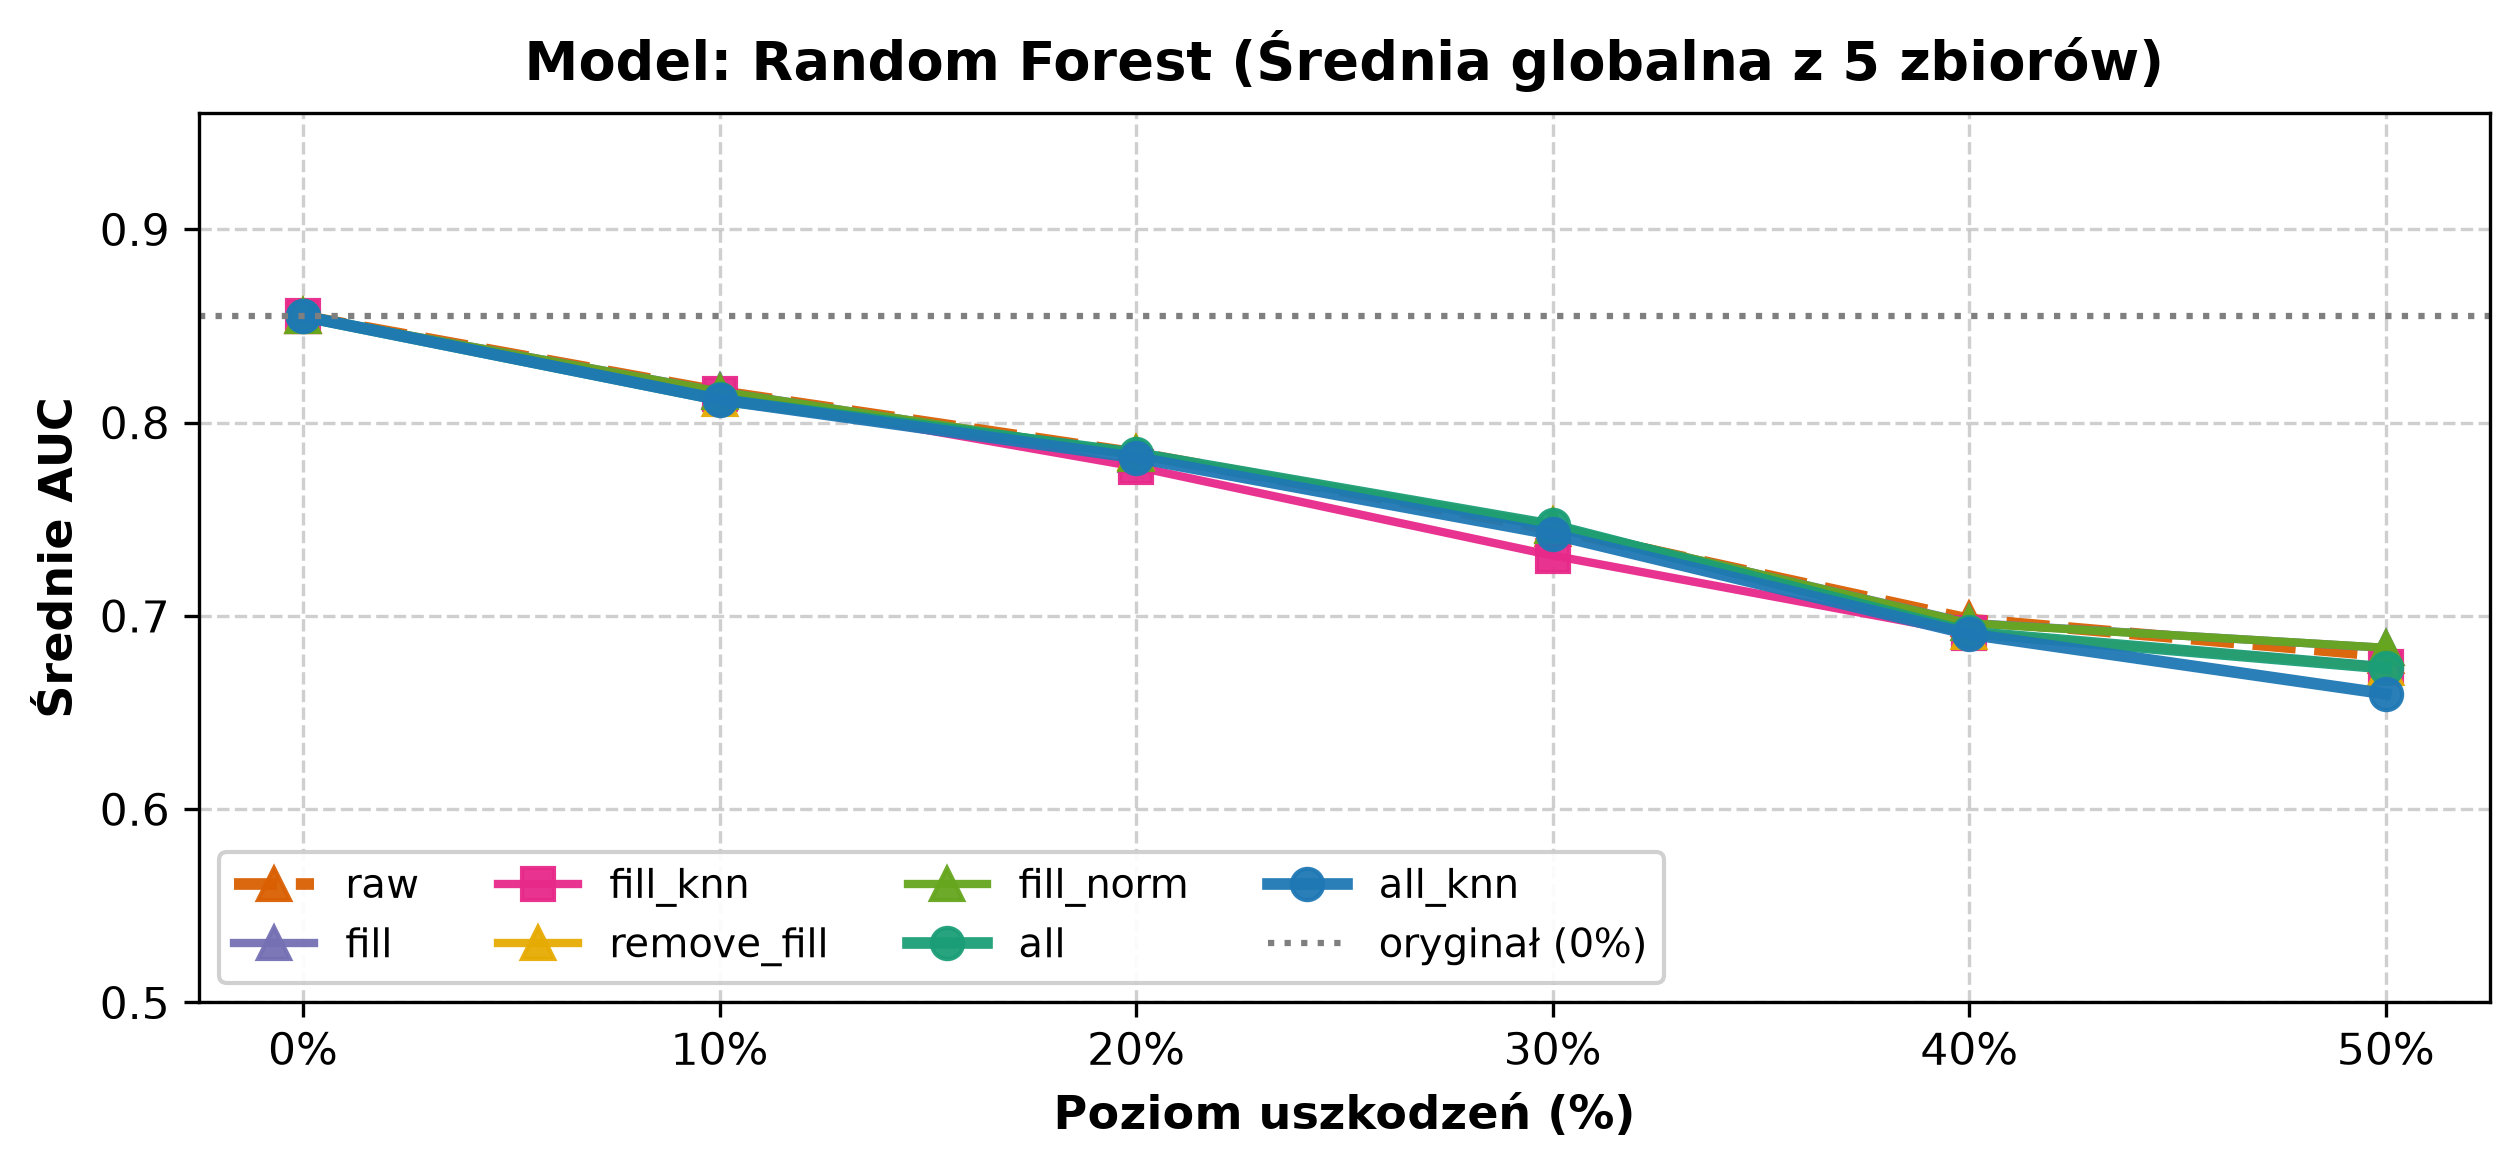
\includegraphics[width=\textwidth]{figures/Wykresy_Zaawansowane/1_Krzywe_Odpornosci/krzywa_zbiorcze_RF.png}
    \caption{Random Forest}
    \label{fig:krzywa_zbiorcze_rf}
\end{subfigure}
\vspace{0.25cm}
\begin{subfigure}[b]{0.92\textwidth}
    \centering
    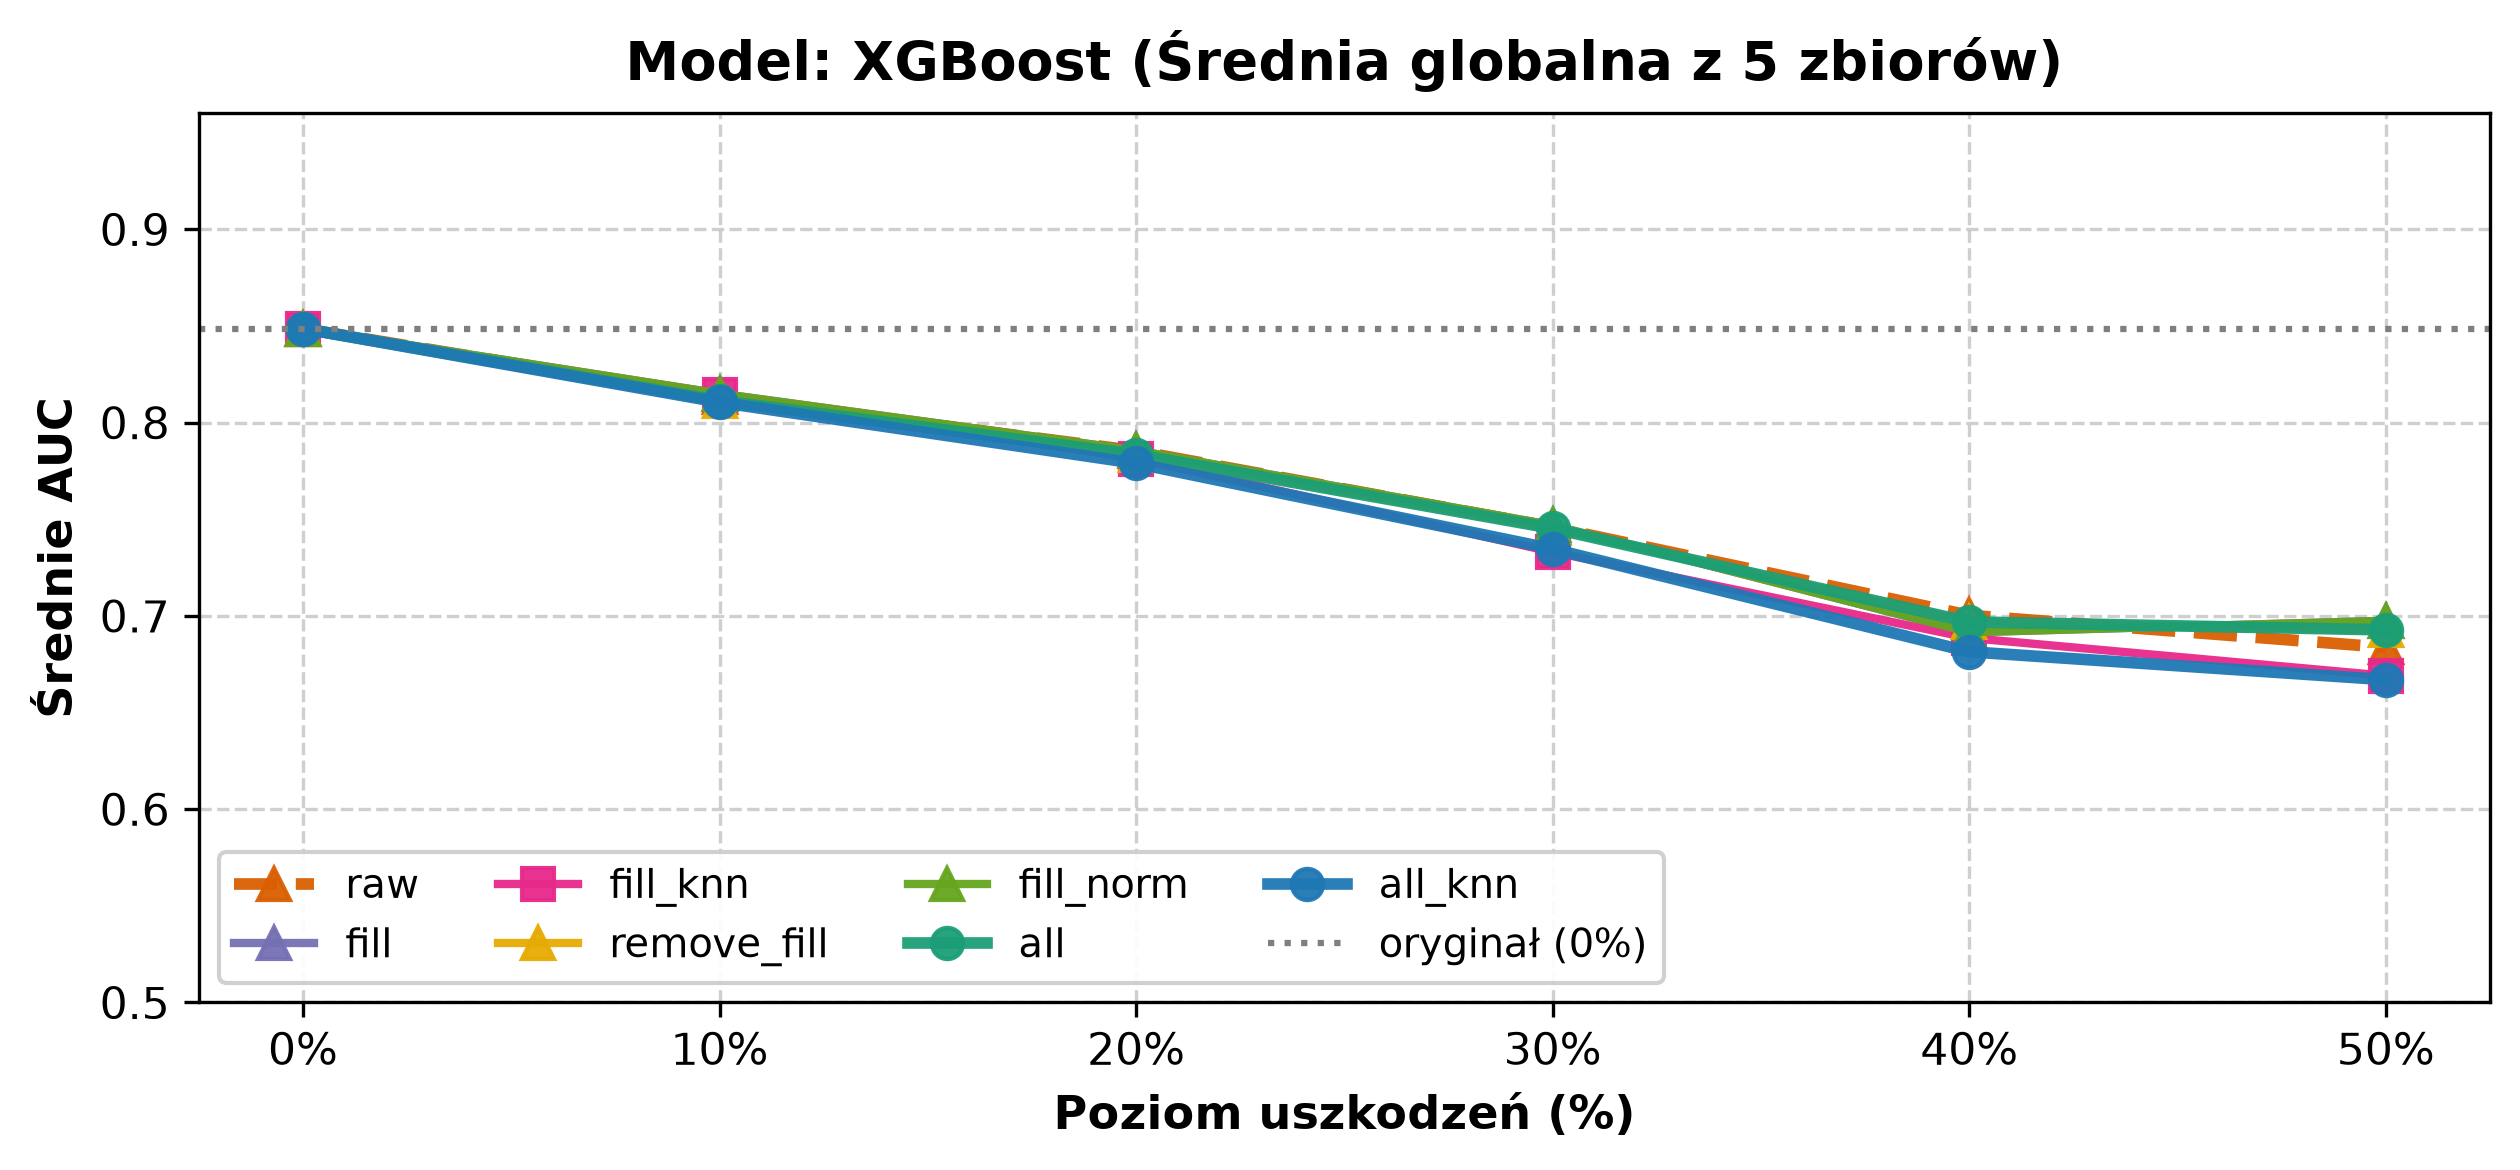
\includegraphics[width=\textwidth]{figures/Wykresy_Zaawansowane/1_Krzywe_Odpornosci/krzywa_zbiorcze_XGBoost.png}
    \caption{XGBoost}
    \label{fig:krzywa_zbiorcze_xgb}
\end{subfigure}
\caption{Zagregowane krzywe odporności modeli zespołowych (uśrednione po 5 badanych zbiorach danych)}
\label{fig:krzywe_zbiorcze_drzewa}
\end{figure}

\begin{figure}[H]
\centering
\begin{subfigure}[b]{0.92\textwidth}
    \centering
    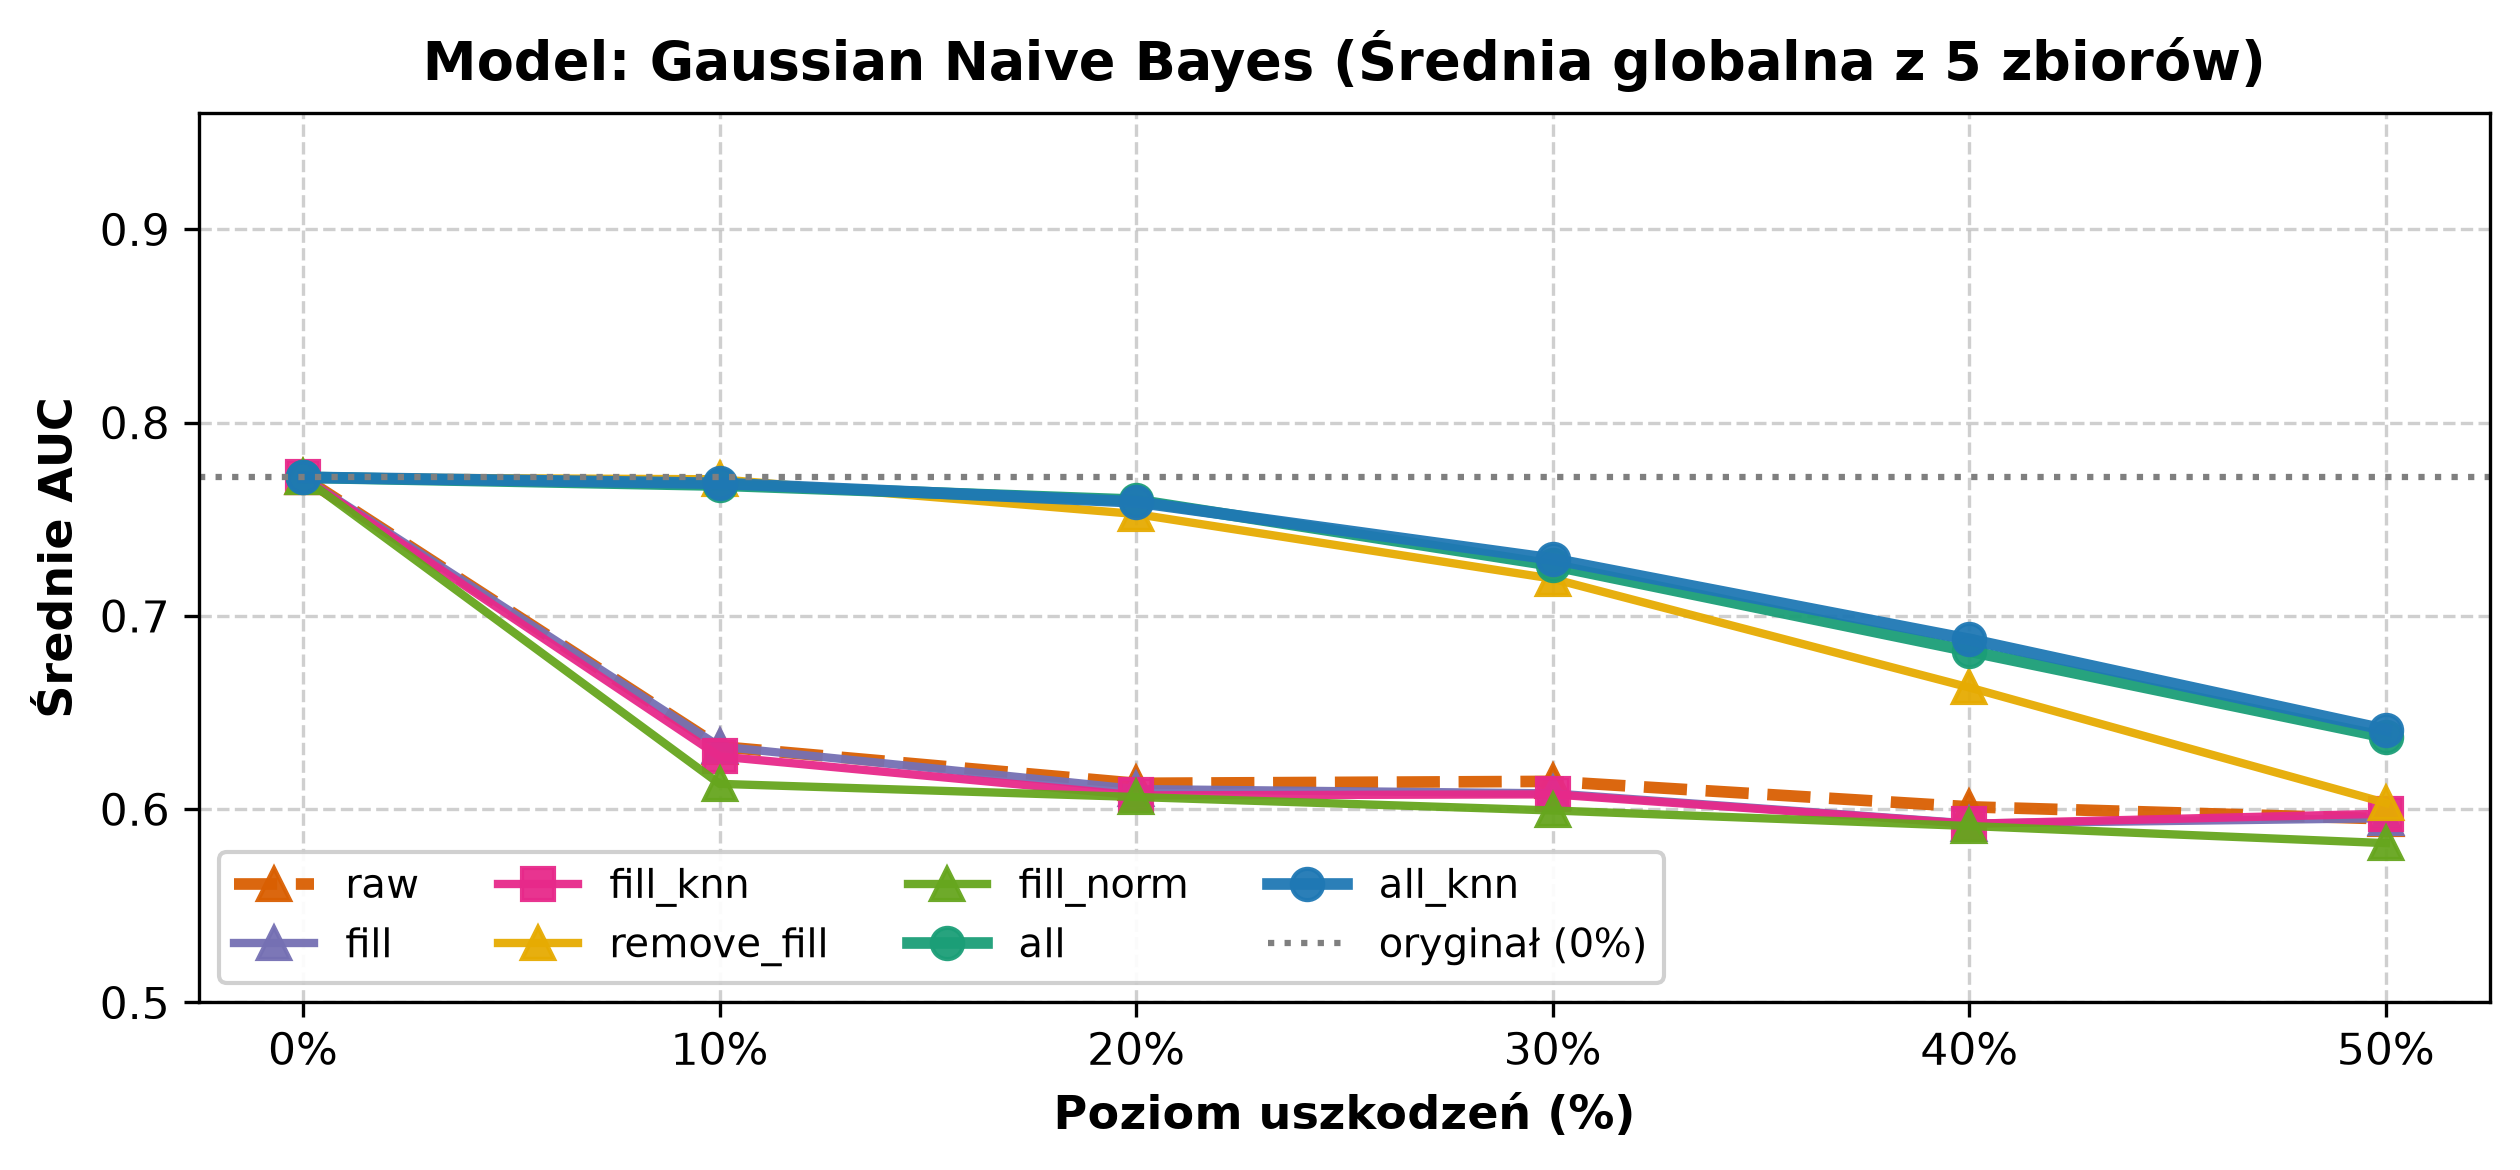
\includegraphics[width=\textwidth]{figures/Wykresy_Zaawansowane/1_Krzywe_Odpornosci/krzywa_zbiorcze_NB.png}
    \caption{Gaussian Naive Bayes}
    \label{fig:krzywa_zbiorcze_nb}
\end{subfigure}
\vspace{0.25cm}
\begin{subfigure}[b]{0.92\textwidth}
    \centering
    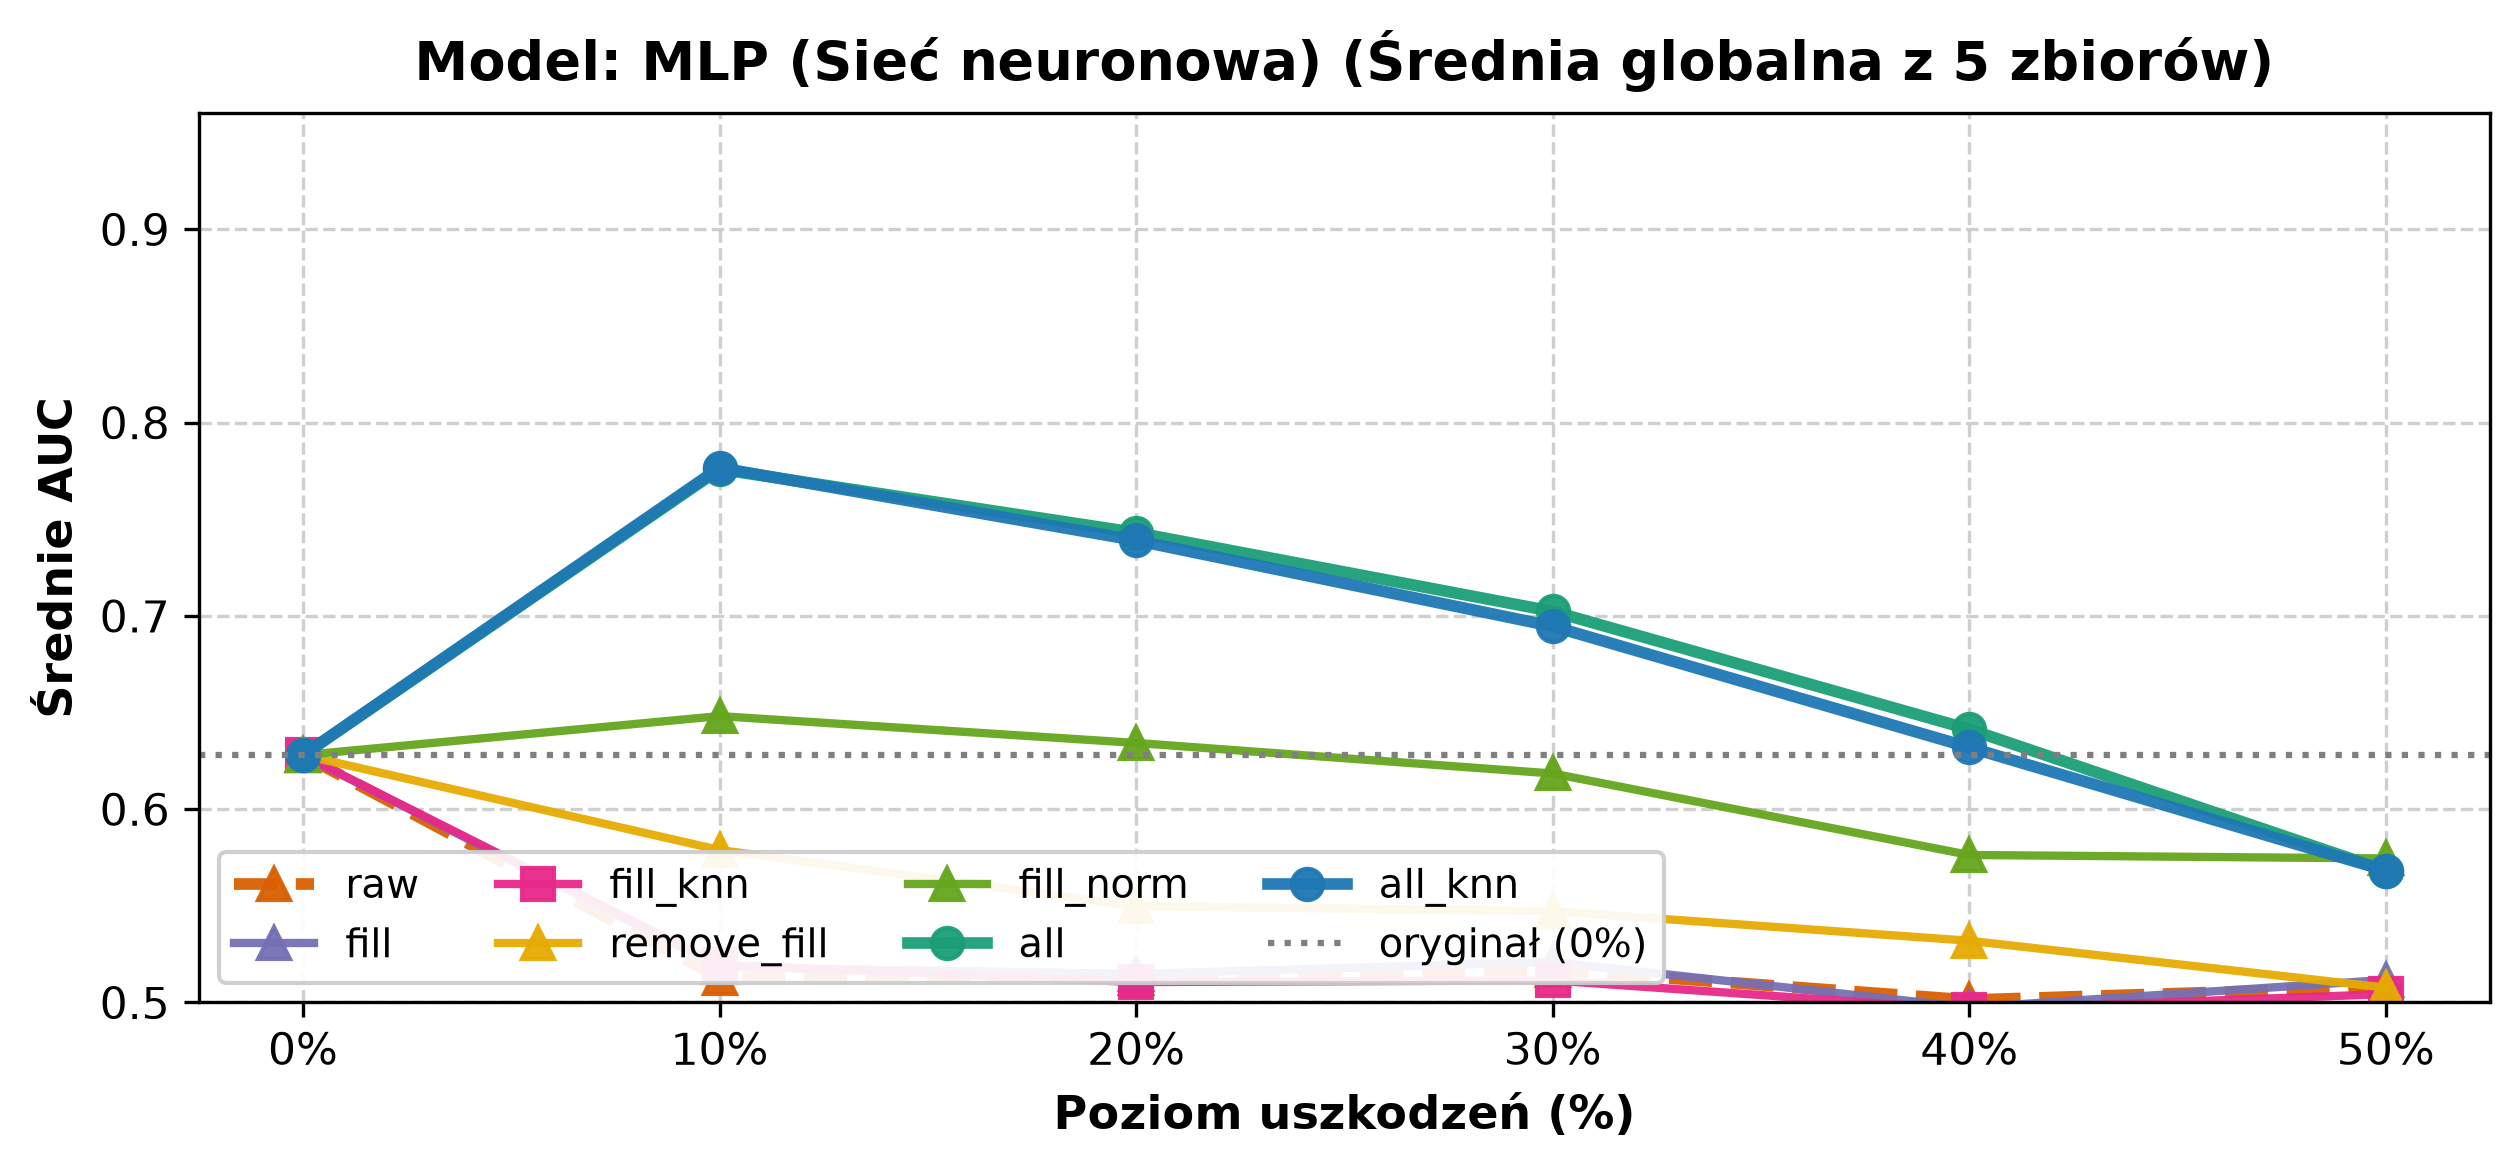
\includegraphics[width=\textwidth]{figures/Wykresy_Zaawansowane/1_Krzywe_Odpornosci/krzywa_zbiorcze_MLP.png}
    \caption{MLP (Sieć neuronowa)}
    \label{fig:krzywa_zbiorcze_mlp}
\end{subfigure}
\caption{Zagregowane krzywe odporności klasyfikatora Bayesa i~sieci MLP (uśrednione po 5 zbiorach danych)}
\label{fig:krzywe_zbiorcze_inne}
\end{figure}

\begin{table}[H]
\centering
\caption{Średnia globalna wartość $\overline{\mathrm{AUC}}$ dla wszystkich badanych zbiorów danych i~modeli w~funkcji poziomu uszkodzeń dla 7 badanych strategii}
\label{tab:zbiorcze_krzywe}
\vspace{0.2cm}
\resizebox{\textwidth}{!}{%
\begin{tabular}{lccccccc}
\toprule
\textbf{Poziom uszkodzeń} & \textbf{\texttt{raw}} & \textbf{\texttt{fill}} & \textbf{\texttt{fill\_knn}} & \textbf{\texttt{remove\_fill}} & \textbf{\texttt{fill\_norm}} & \textbf{\texttt{all}} & \textbf{\texttt{all\_knn}} \\
\midrule
10\% & $0{,}6936$ & $0{,}6955$ & $0{,}6940$ & $0{,}7432$ & $0{,}7231$ & $0{,}7917$ & $\mathbf{0{,}7919}$ \\
20\% & $0{,}6739$ & $0{,}6735$ & $0{,}6690$ & $0{,}7175$ & $0{,}7024$ & $\mathbf{0{,}7676}$ & $0{,}7647$ \\
30\% & $0{,}6555$ & $0{,}6556$ & $0{,}6458$ & $0{,}6896$ & $0{,}6778$ & $\mathbf{0{,}7301}$ & $0{,}7252$ \\
40\% & $0{,}6252$ & $0{,}6194$ & $0{,}6171$ & $0{,}6458$ & $0{,}6388$ & $\mathbf{0{,}6779}$ & $0{,}6729$ \\
50\% & $0{,}6165$ & $0{,}6219$ & $0{,}6112$ & $0{,}6192$ & $0{,}6344$ & $\mathbf{0{,}6428}$ & $0{,}6340$ \\
\bottomrule
\end{tabular}%
}
\end{table}

Wykres zbiorczy uwidacznia fundamentalną prawidłowość: brak procedur czyszczących (\textit{raw}, oznaczony linią pomarańczową) prowadzi do gwałtownej degradacji jakości predykcji wszystkich modeli. Zastosowanie pełnego potoku czyszczącego (\textit{all} oraz \textit{all\_knn}) skutecznie hamuje spadek AUC, zachowując najwyższą użyteczność decyzyjną modeli nawet przy $50\%$ stopniu uszkodzenia atrybutów.

\section{Szczegółowa analiza wyników na poszczególnych zbiorach danych}

\subsection{Ocena na zbiorze „Zapalenia naczyń”}
Zbiór kliniczny pacjentów z~zapaleniem naczyń charakteryzuje się dużą liczbą cech ($143$) oraz obecnością kluczowych markerów stanu zapalnego.

\begin{table}[H]
\centering
\caption{Wyniki $\overline{\mathrm{AUC}}$ na zbiorze „Zapalenia naczyń” dla wszystkich poziomów degradacji}
\label{tab:wyniki_zapalenia}
\vspace{0.2cm}
\resizebox{\textwidth}{!}{%
\begin{tabular}{llccccccc}
\toprule
\textbf{Model} & \textbf{Poziom} & \textbf{\texttt{raw}} & \textbf{\texttt{fill}} & \textbf{\texttt{fill\_knn}} & \textbf{\texttt{remove\_fill}} & \textbf{\texttt{fill\_norm}} & \textbf{\texttt{all}} & \textbf{\texttt{all\_knn}} \\
\midrule
\textbf{RF}      & 10\% & $0{,}9096$ & $\mathbf{0{,}9158}$ & $0{,}9137$ & $0{,}9080$ & $0{,}9157$ & $0{,}9079$ & $0{,}9096$ \\
                 & 20\% & $0{,}8900$ & $\mathbf{0{,}8944}$ & $0{,}8893$ & $0{,}8873$ & $0{,}8943$ & $0{,}8872$ & $0{,}8853$ \\
                 & 30\% & $0{,}8819$ & $\mathbf{0{,}8848}$ & $0{,}8753$ & $0{,}8549$ & $0{,}8847$ & $0{,}8550$ & $0{,}8565$ \\
                 & 40\% & $\mathbf{0{,}8557}$ & $0{,}8501$ & $0{,}8476$ & $0{,}8213$ & $0{,}8500$ & $0{,}8214$ & $0{,}8234$ \\
                 & 50\% & $0{,}8314$ & $\mathbf{0{,}8419}$ & $0{,}8365$ & $0{,}7853$ & $\mathbf{0{,}8419}$ & $0{,}7855$ & $0{,}7723$ \\
\midrule
\textbf{XGBoost} & 10\% & $0{,}9140$ & $\mathbf{0{,}9219}$ & $0{,}9198$ & $0{,}9134$ & $\mathbf{0{,}9219}$ & $0{,}9134$ & $0{,}9164$ \\
                 & 20\% & $0{,}8916$ & $\mathbf{0{,}8984}$ & $0{,}8929$ & $0{,}8902$ & $\mathbf{0{,}8984}$ & $0{,}8902$ & $0{,}8880$ \\
                 & 30\% & $\mathbf{0{,}8710}$ & $0{,}8698$ & $0{,}8616$ & $0{,}8465$ & $0{,}8698$ & $0{,}8465$ & $0{,}8508$ \\
                 & 40\% & $\mathbf{0{,}8321}$ & $0{,}8114$ & $0{,}8147$ & $0{,}8140$ & $0{,}8114$ & $0{,}8140$ & $0{,}8047$ \\
                 & 50\% & $0{,}7835$ & $\mathbf{0{,}8050}$ & $0{,}7928$ & $0{,}7784$ & $\mathbf{0{,}8050}$ & $0{,}7784$ & $0{,}7730$ \\
\midrule
\textbf{NB}      & 10\% & $0{,}6704$ & $0{,}6695$ & $0{,}6624$ & $\mathbf{0{,}8354}$ & $0{,}5833$ & $0{,}8255$ & $0{,}8262$ \\
                 & 20\% & $0{,}6150$ & $0{,}6145$ & $0{,}5965$ & $0{,}7916$ & $0{,}5945$ & $0{,}8308$ & $\mathbf{0{,}8321}$ \\
                 & 30\% & $0{,}6540$ & $0{,}6542$ & $0{,}6225$ & $0{,}7862$ & $0{,}5821$ & $\mathbf{0{,}8221}$ & $0{,}8218$ \\
                 & 40\% & $0{,}6056$ & $0{,}6050$ & $0{,}5756$ & $0{,}7108$ & $0{,}5952$ & $0{,}7973$ & $\mathbf{0{,}7982}$ \\
                 & 50\% & $0{,}5855$ & $0{,}5846$ & $0{,}5868$ & $0{,}5926$ & $0{,}5664$ & $0{,}7551$ & $\mathbf{0{,}7578}$ \\
\midrule
\textbf{MLP}     & 10\% & $0{,}6105$ & $0{,}6445$ & $0{,}6431$ & $0{,}5996$ & $\mathbf{0{,}8758}$ & $0{,}8632$ & $0{,}8721$ \\
                 & 20\% & $0{,}5660$ & $0{,}5692$ & $0{,}5619$ & $0{,}5691$ & $\mathbf{0{,}8526}$ & $0{,}8401$ & $0{,}8390$ \\
                 & 30\% & $0{,}5826$ & $0{,}5854$ & $0{,}5504$ & $0{,}5594$ & $\mathbf{0{,}8343}$ & $0{,}8131$ & $0{,}8103$ \\
                 & 40\% & $0{,}5414$ & $0{,}5136$ & $0{,}5162$ & $0{,}5496$ & $\mathbf{0{,}7965}$ & $0{,}7601$ & $0{,}7485$ \\
                 & 50\% & $0{,}5576$ & $0{,}5556$ & $0{,}5473$ & $0{,}5278$ & $\mathbf{0{,}7212}$ & $0{,}6545$ & $0{,}6738$ \\
\bottomrule
\end{tabular}%
}
\end{table}

\begin{figure}[H]
\centering
\begin{subfigure}[b]{0.92\textwidth}
    \centering
    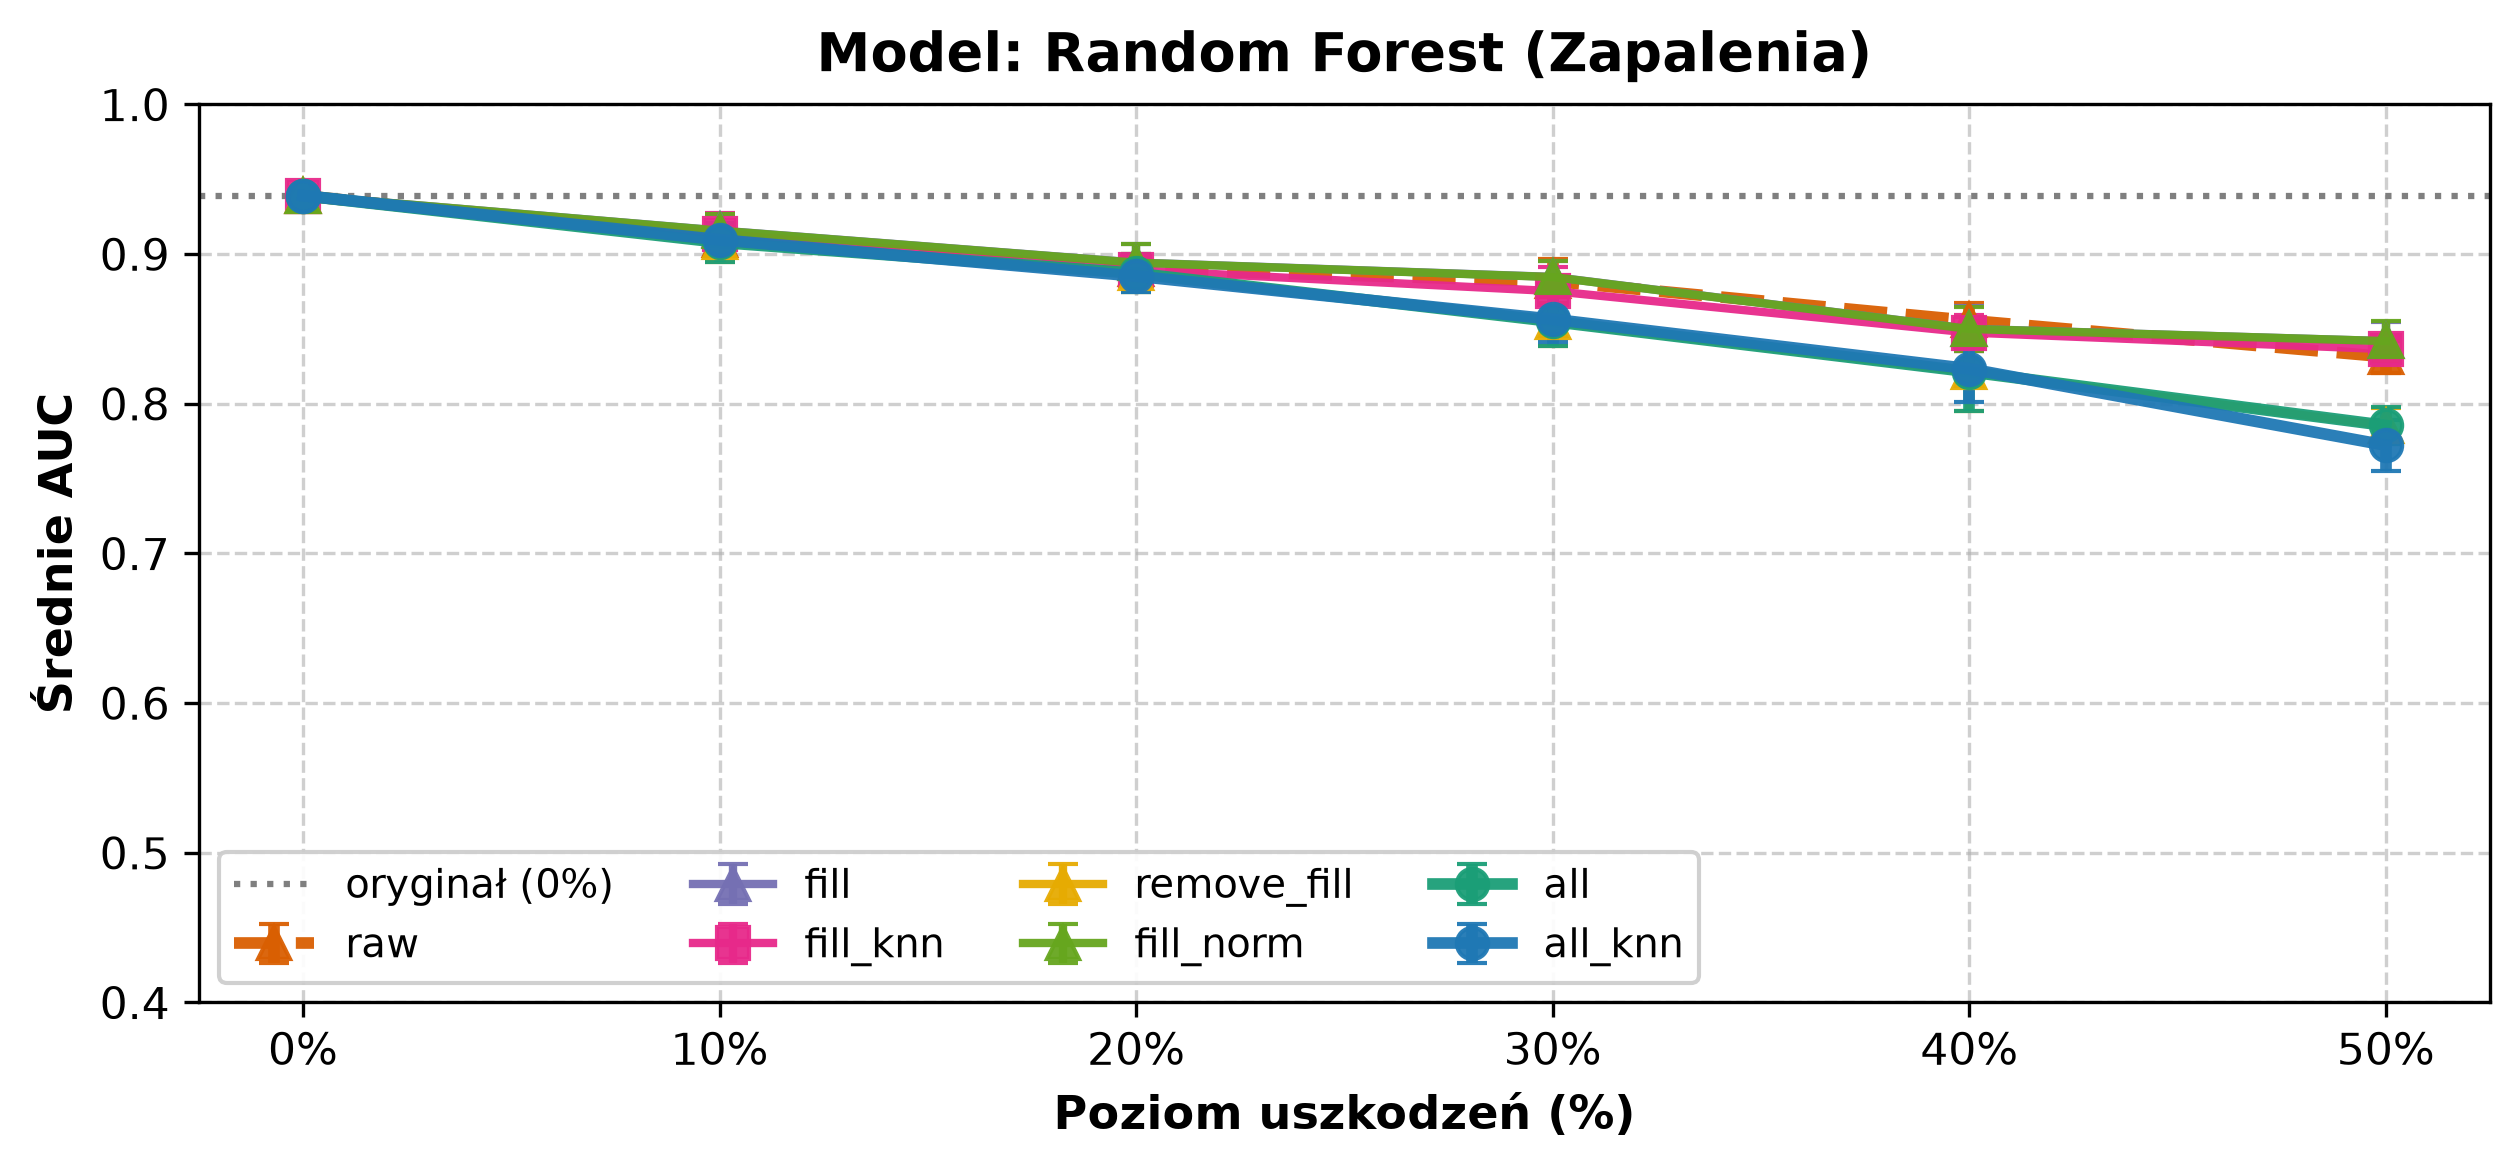
\includegraphics[width=\textwidth]{figures/Wykresy_Zaawansowane/1_Krzywe_Odpornosci/krzywa_zapalenia_RF.png}
    \caption{Random Forest}
    \label{fig:odp_zap_rf}
\end{subfigure}
\vspace{0.25cm}
\begin{subfigure}[b]{0.92\textwidth}
    \centering
    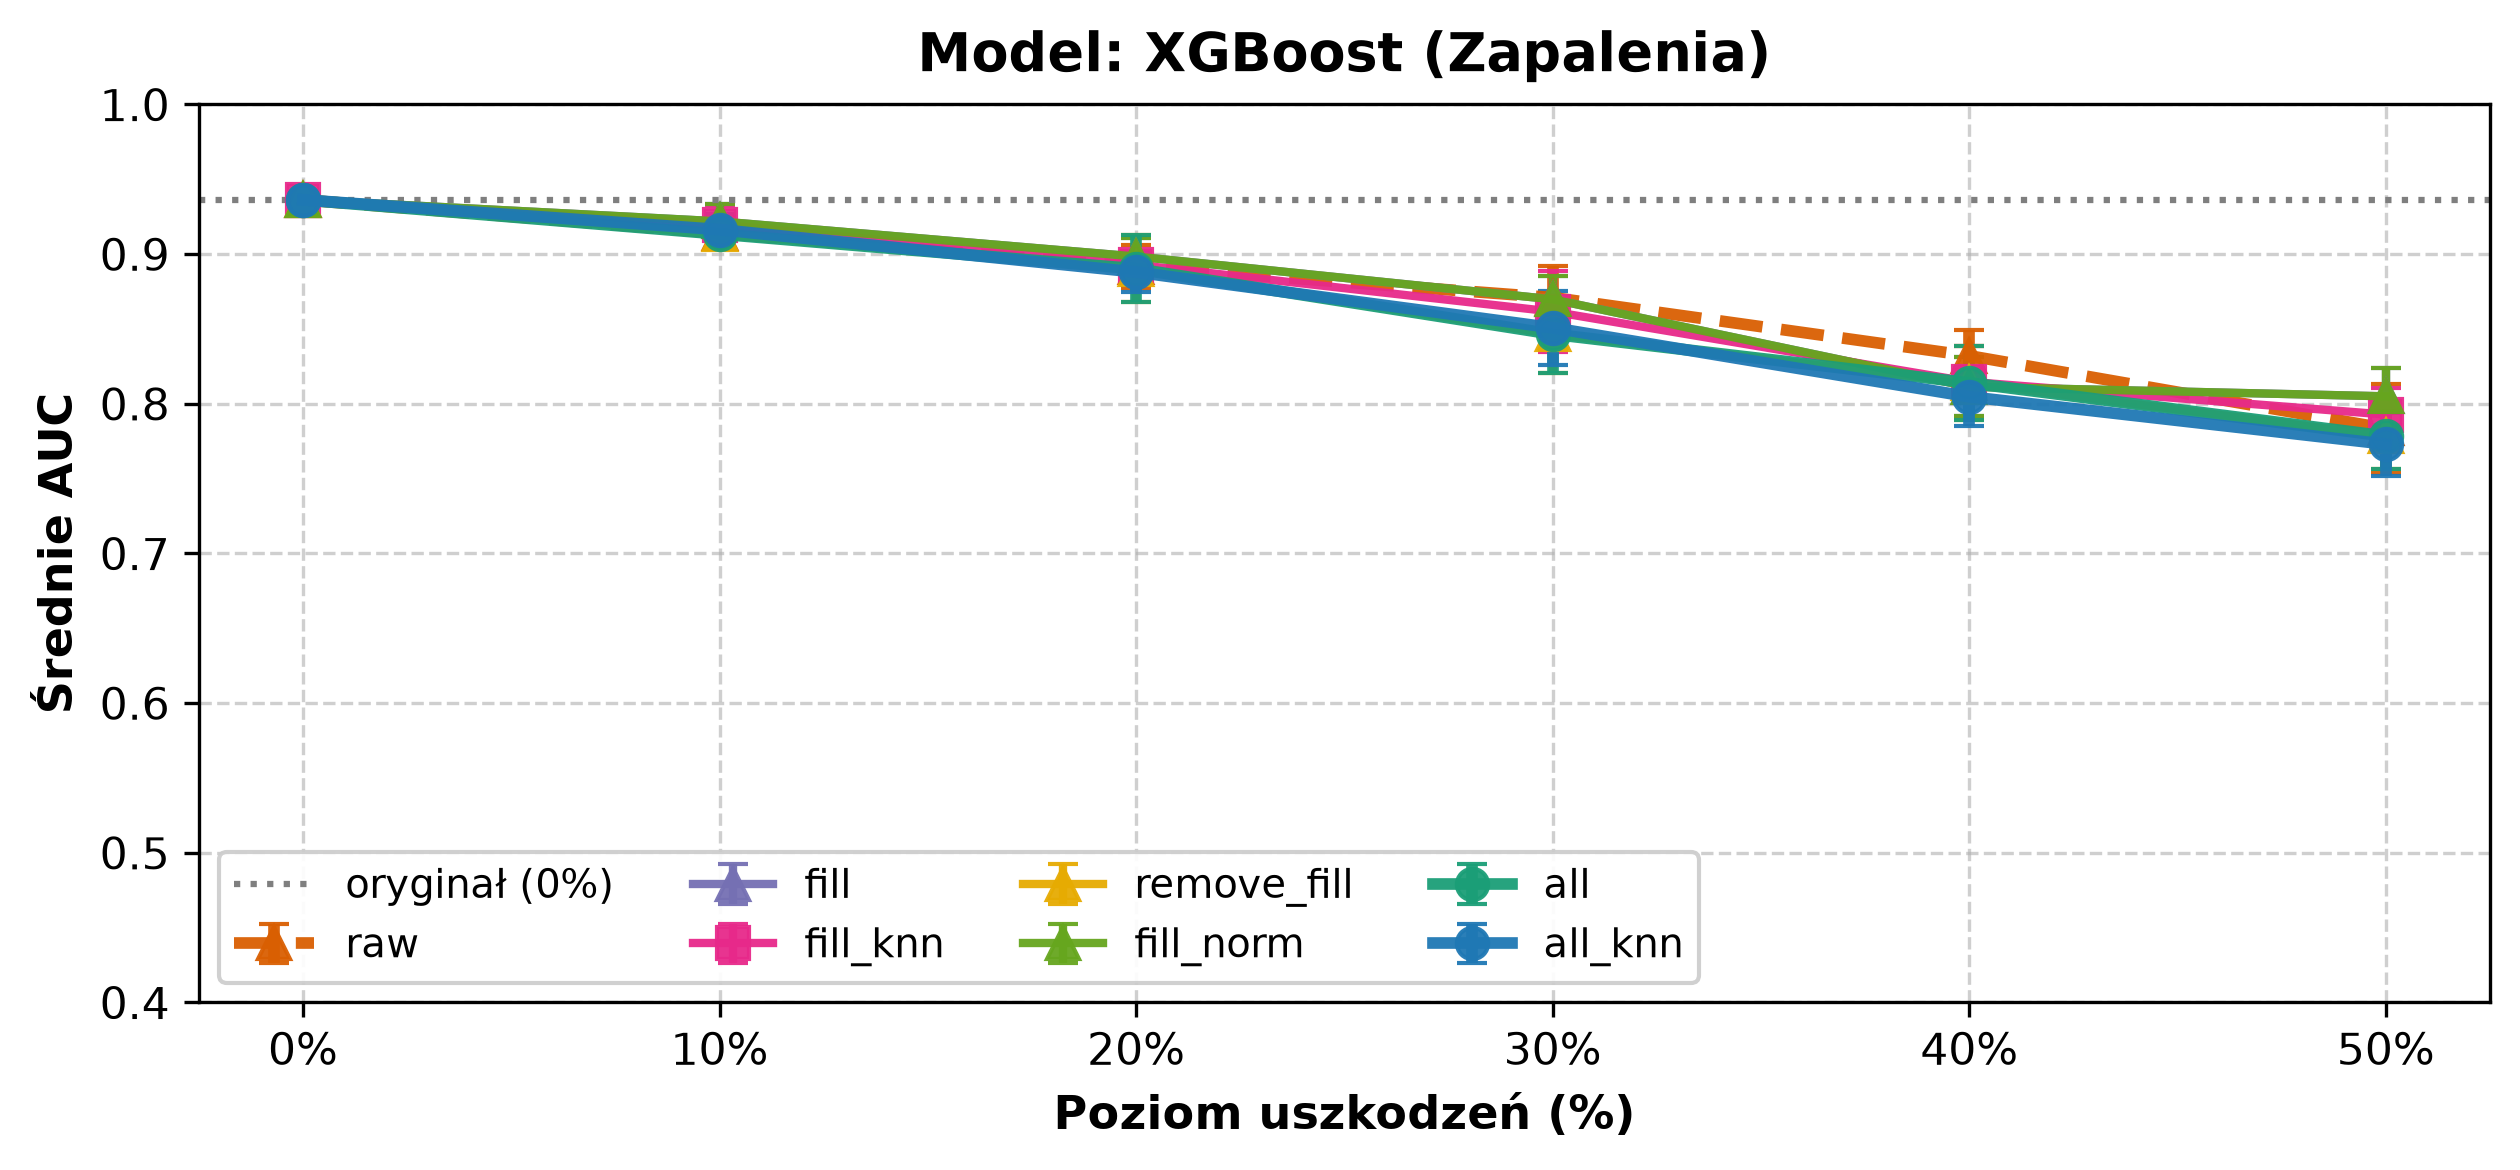
\includegraphics[width=\textwidth]{figures/Wykresy_Zaawansowane/1_Krzywe_Odpornosci/krzywa_zapalenia_XGBoost.png}
    \caption{XGBoost}
    \label{fig:odp_zap_xgb}
\end{subfigure}
\caption{Krzywe odporności modeli zespołowych na zbiorze „Zapalenia naczyń”}
\label{fig:odpornosc_zapalenia_drzewa}
\end{figure}

\begin{figure}[H]
\centering
\begin{subfigure}[b]{0.92\textwidth}
    \centering
    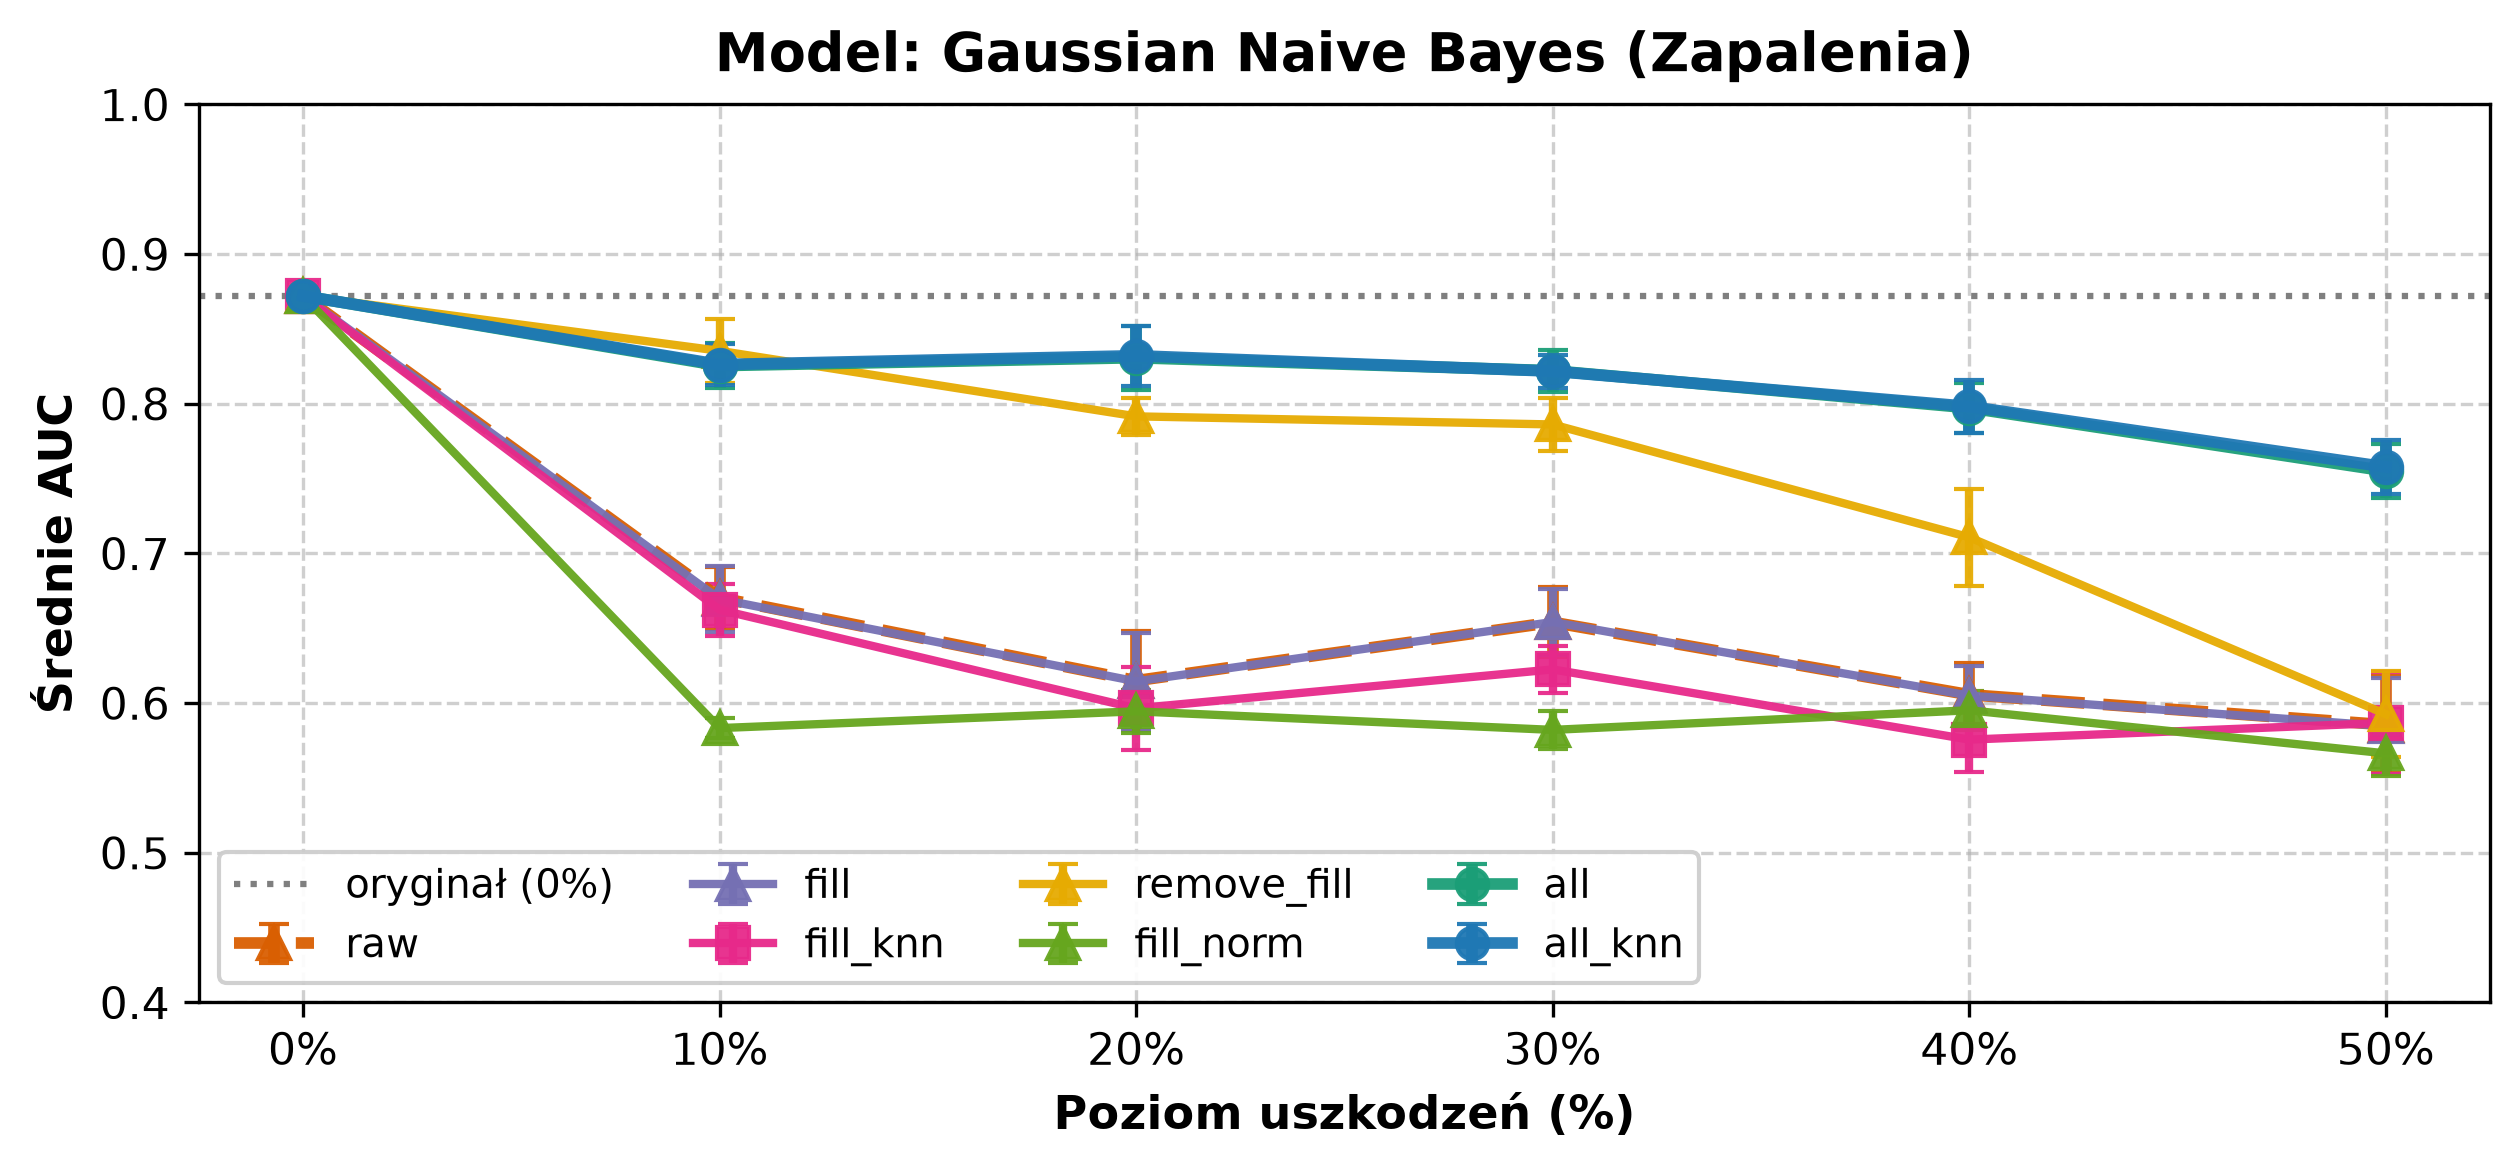
\includegraphics[width=\textwidth]{figures/Wykresy_Zaawansowane/1_Krzywe_Odpornosci/krzywa_zapalenia_NB.png}
    \caption{Gaussian Naive Bayes}
    \label{fig:odp_zap_nb}
\end{subfigure}
\vspace{0.25cm}
\begin{subfigure}[b]{0.92\textwidth}
    \centering
    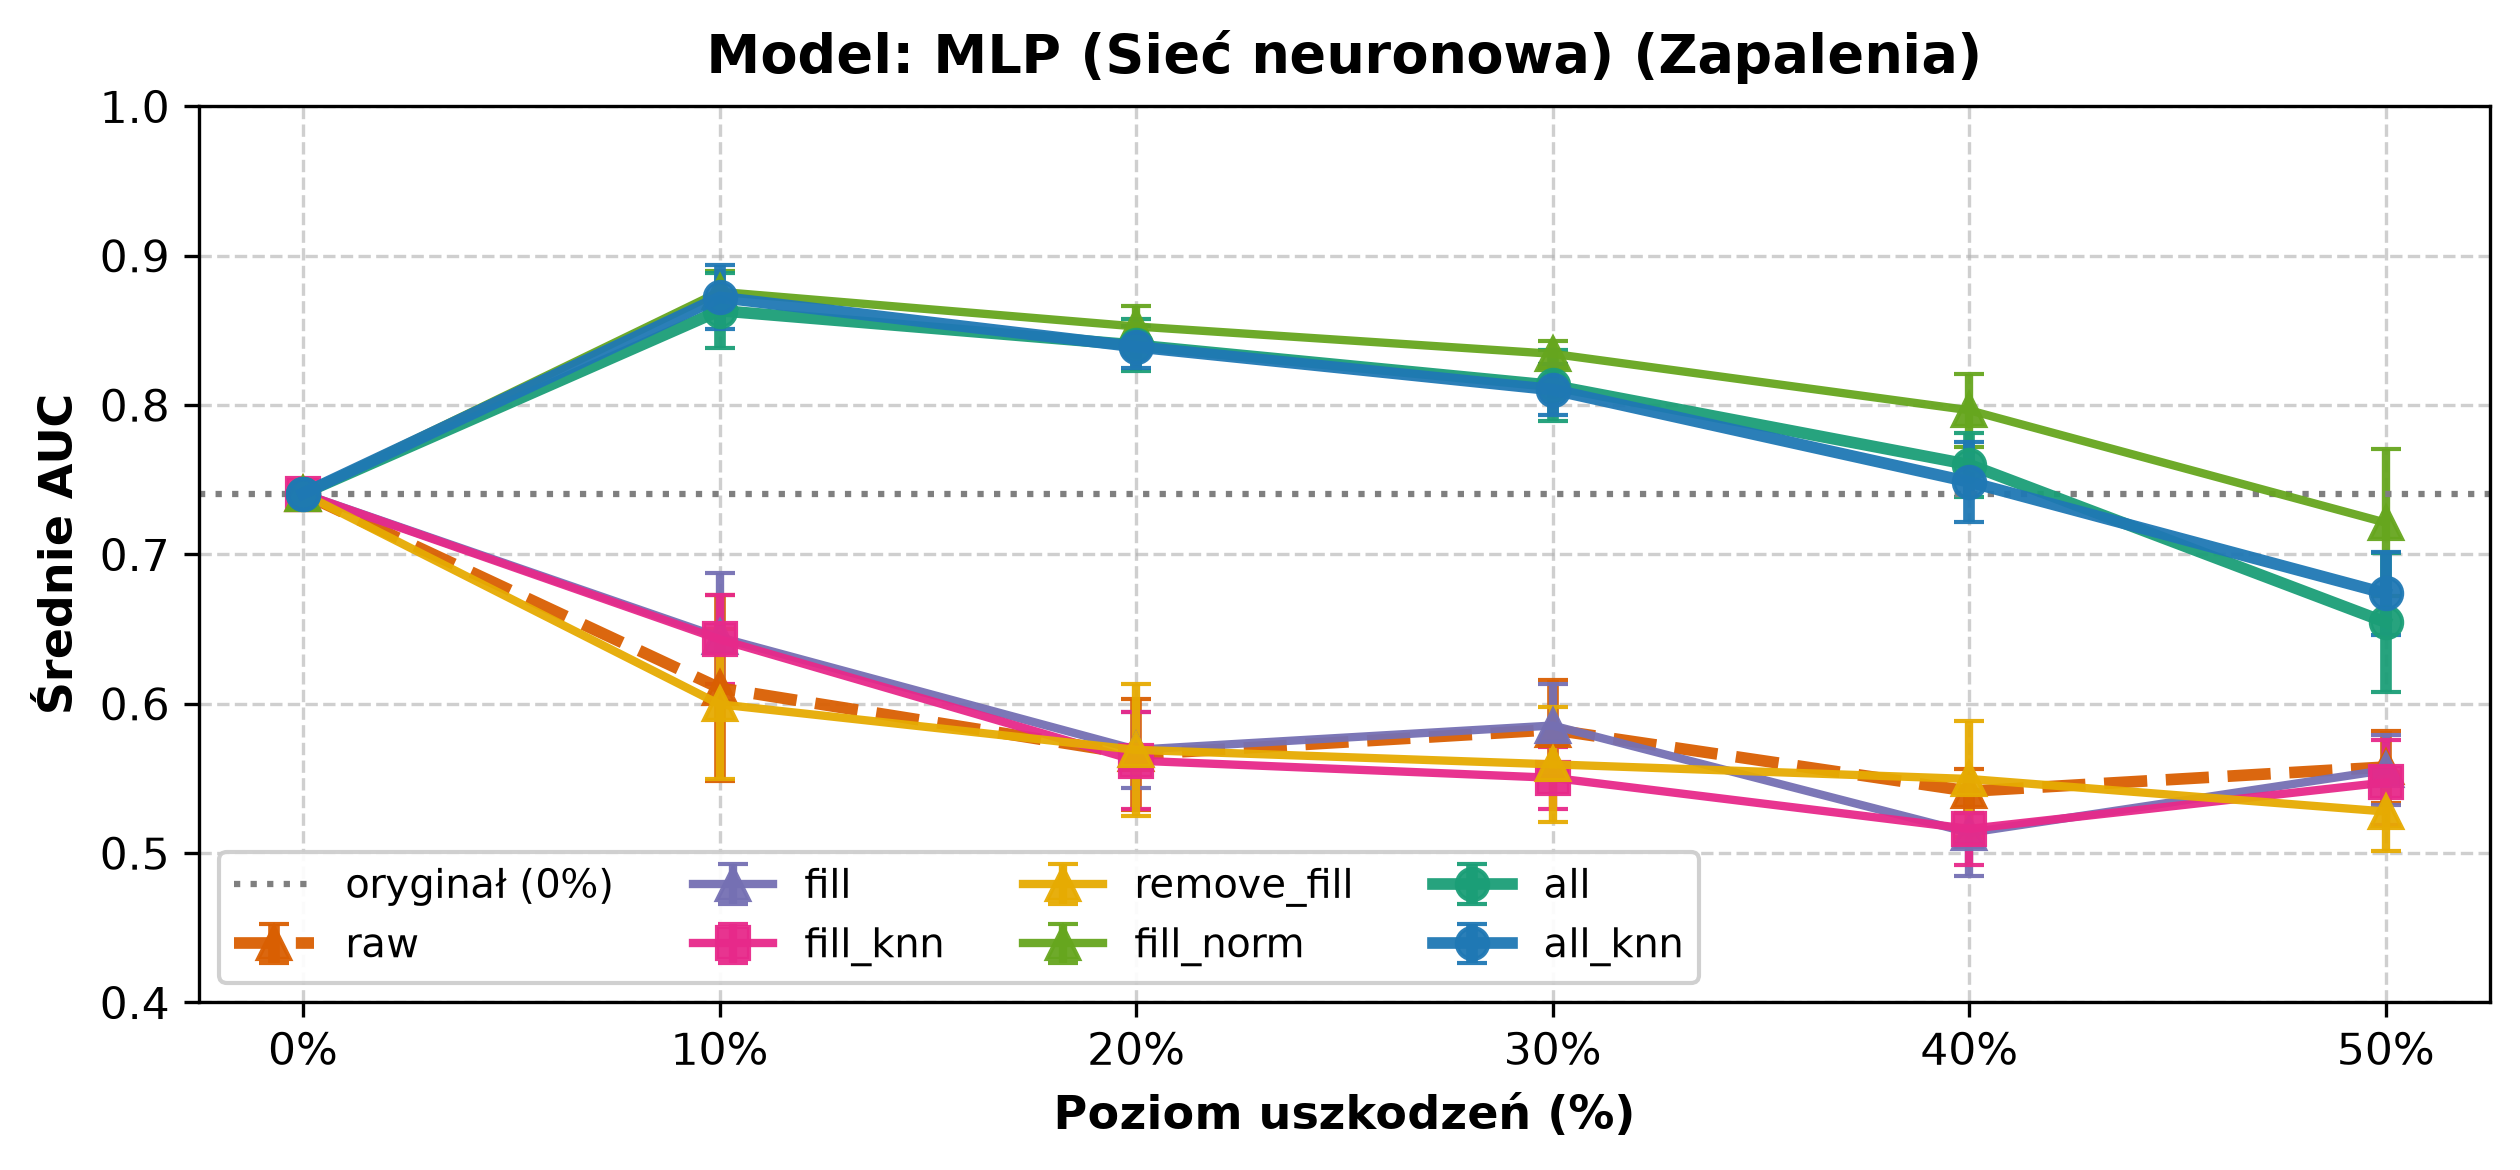
\includegraphics[width=\textwidth]{figures/Wykresy_Zaawansowane/1_Krzywe_Odpornosci/krzywa_zapalenia_MLP.png}
    \caption{MLP (Sieć neuronowa)}
    \label{fig:odp_zap_mlp}
\end{subfigure}
\caption{Krzywe odporności klasyfikatora Bayesa i~sieci MLP na zbiorze „Zapalenia naczyń”}
\label{fig:odpornosc_zapalenia_inne}
\end{figure}

\begin{figure}[H]
\centering
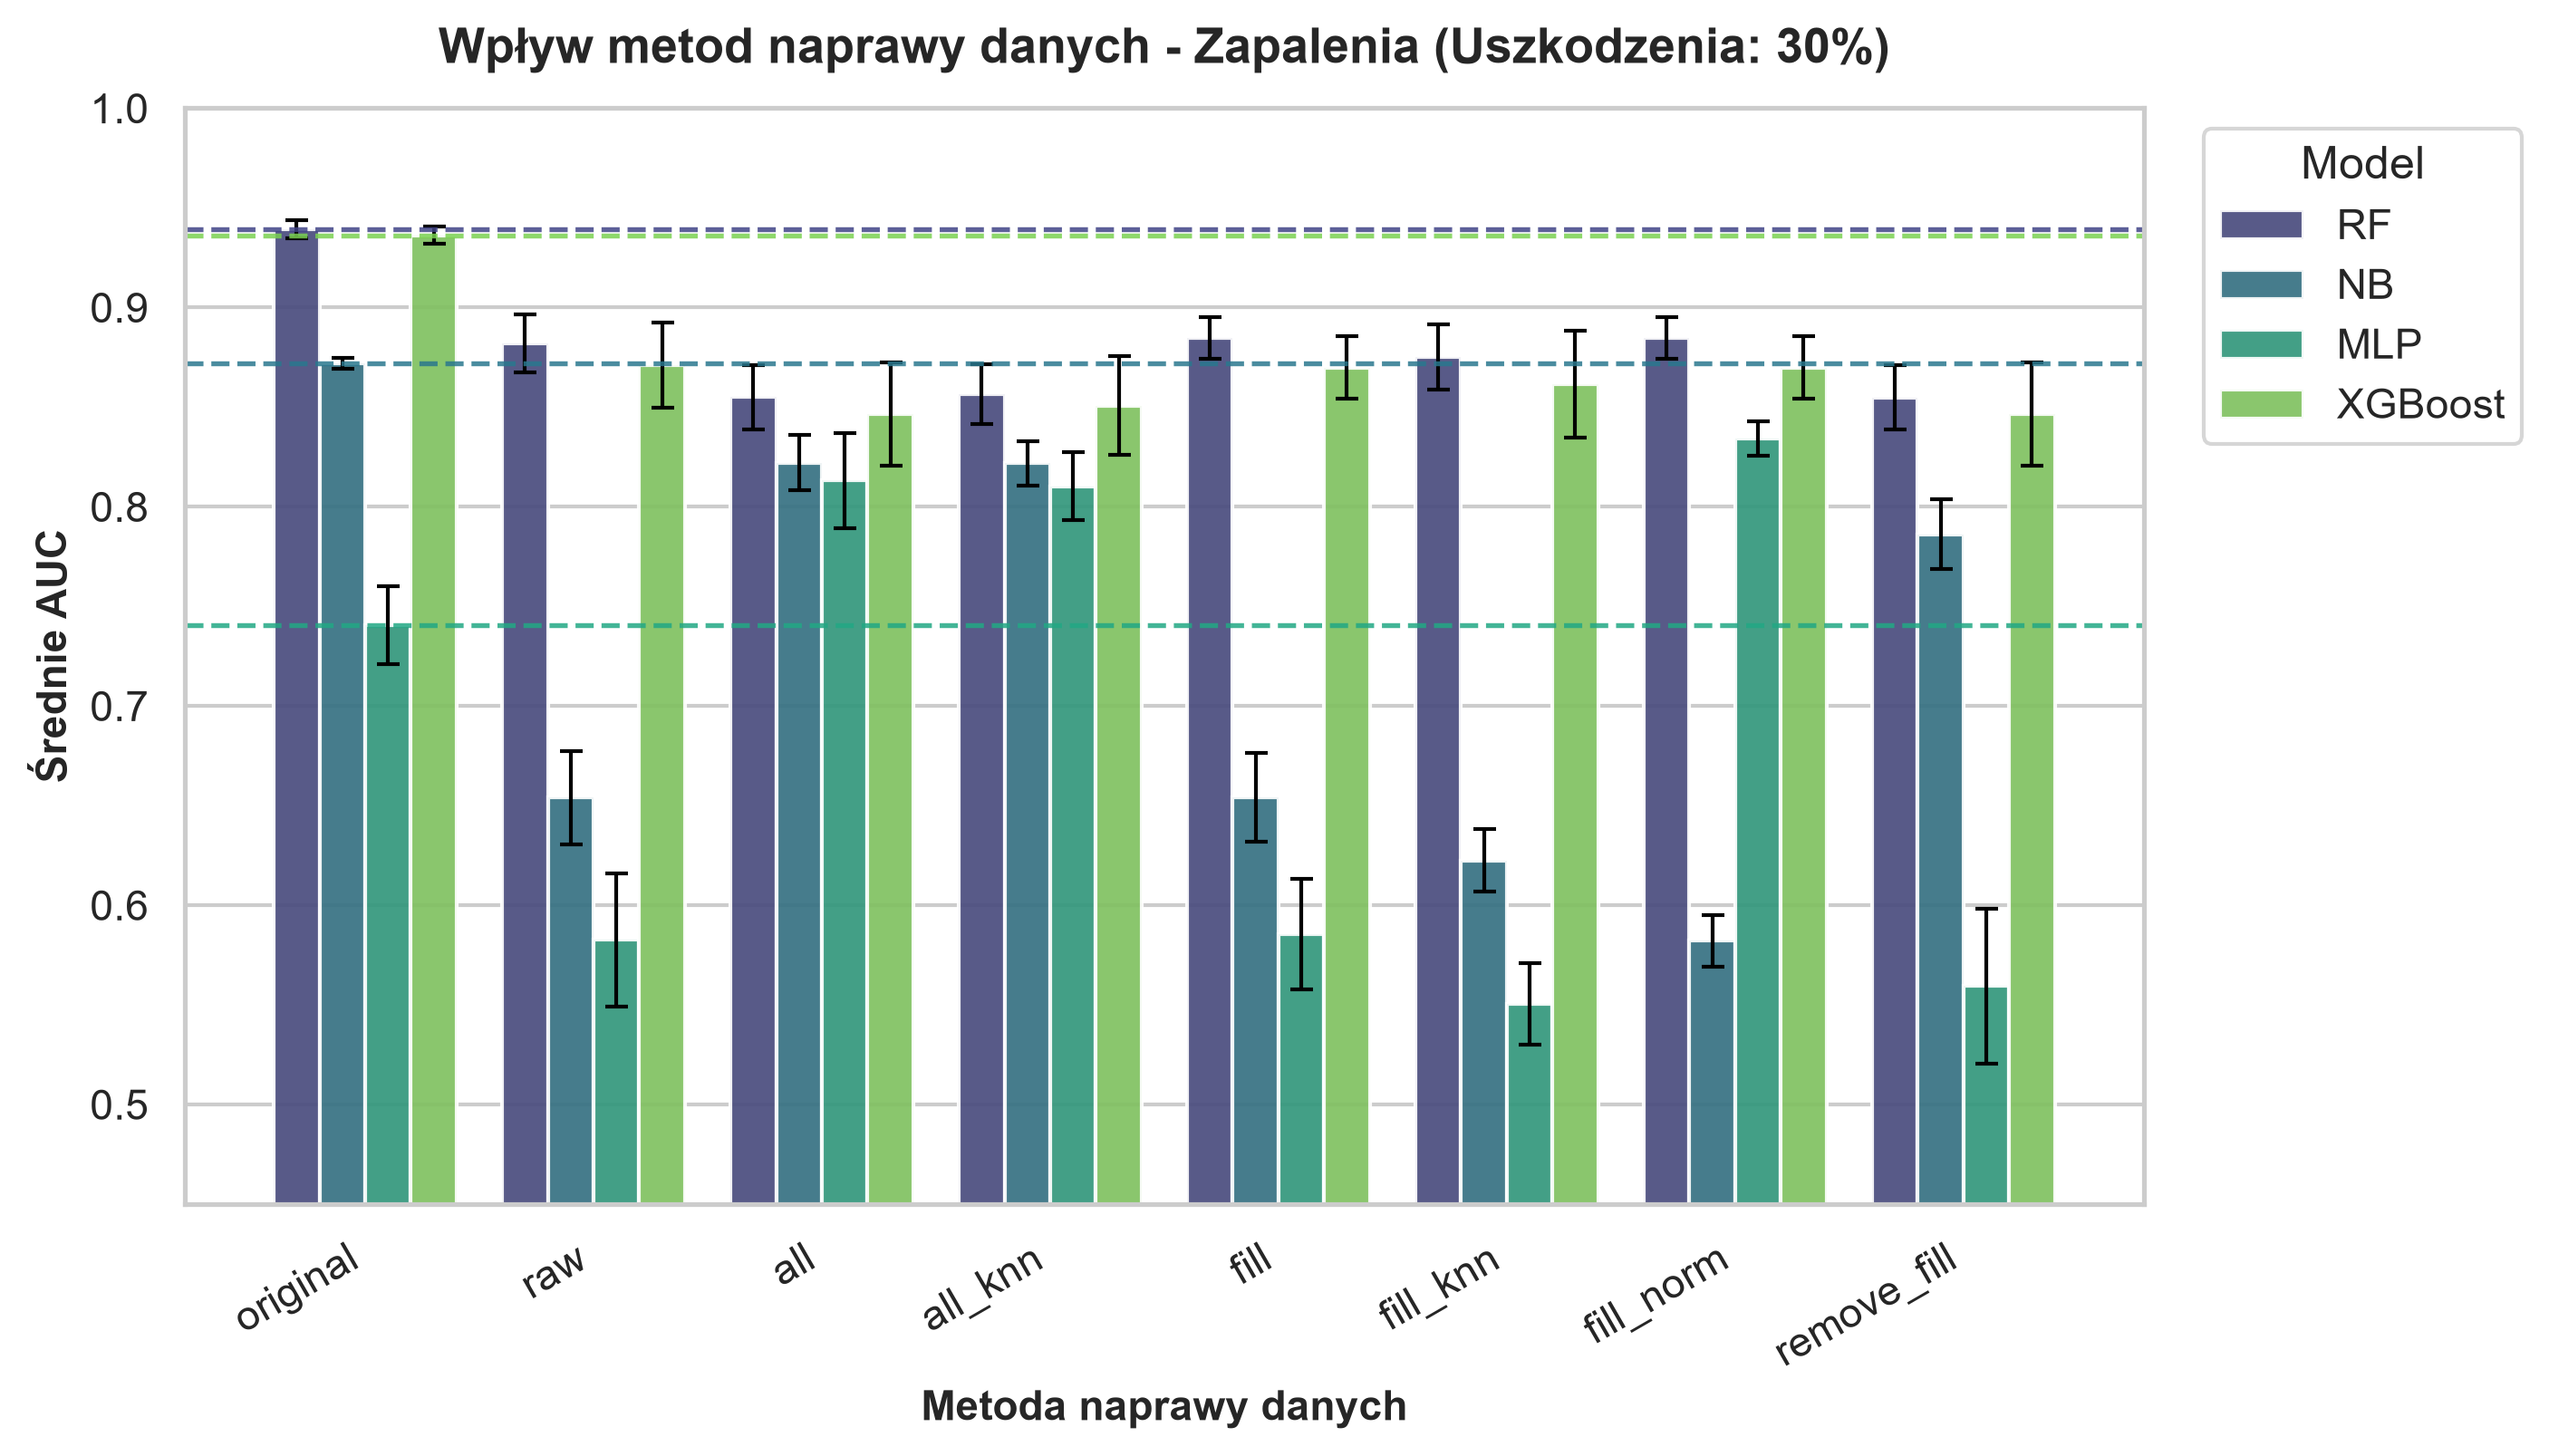
\includegraphics[width=0.95\textwidth]{figures/Wykresy_full/zapalenia/zapalenia_30proc.png}
\caption{Porównanie skuteczności metod czyszczenia danych wraz ze słupkami błędów na zbiorze „Zapalenia naczyń” przy poziomie uszkodzeń 30\%}
\label{fig:slupkowy_zapalenia_30}
\end{figure}

Wyniki eksperymentalne na zbiorze „Zapalenia naczyń” (Tabela~\ref{tab:wyniki_zapalenia}) jednoznacznie wskazują, że zniekształcenie atrybutów przy braku czyszczenia obniża AUC modelu Random Forest z~$0{,}939$ do $0{,}831$ przy uszkodzeniu $50\%$. Zastosowanie potoku \textit{fill} pozwala odzyskać stabilność ($0{,}842$), a~w~przypadku sieci MLP wdrożenie potoku \textit{fill\_norm} podnosi AUC z~$0{,}558$ aż do $0{,}721$ (zysk $\Delta \mathrm{AUC} = +0{,}163$).

\subsection{Ocena na zbiorze „Serce” (Heart Disease)}
Zbiór kardiologiczny stanowi reprezentatywny przykład danych o~zrównoważonej liczbie cech ciągłych i~kategorycznych ($13$ atrybutów). Wyniki liczbowe skuteczności klasyfikatorów zestawiono w~tabeli~\ref{tab:wyniki_serce}. Dynamikę zachowania modeli oraz szczegółowe porównanie słupkowe przy uszkodzeniu $30\%$ przedstawiono na rysunkach~\ref{fig:odpornosc_serce_drzewa}, \ref{fig:odpornosc_serce_inne} i~\ref{fig:slupkowy_serce_30}.

\begin{table}[H]
\centering
\caption{Wyniki $\overline{\mathrm{AUC}}$ na zbiorze „Serce” dla wszystkich poziomów degradacji}
\label{tab:wyniki_serce}
\vspace{0.2cm}
\resizebox{\textwidth}{!}{%
\begin{tabular}{llccccccc}
\toprule
\textbf{Model} & \textbf{Poziom} & \textbf{\texttt{raw}} & \textbf{\texttt{fill}} & \textbf{\texttt{fill\_knn}} & \textbf{\texttt{remove\_fill}} & \textbf{\texttt{fill\_norm}} & \textbf{\texttt{all}} & \textbf{\texttt{all\_knn}} \\
\midrule
\textbf{RF}      & 10\% & $\mathbf{0{,}8808}$ & $0{,}8767$ & $0{,}8804$ & $0{,}8757$ & $0{,}8768$ & $0{,}8750$ & $0{,}8793$ \\
                 & 20\% & $\mathbf{0{,}8592}$ & $0{,}8466$ & $0{,}8434$ & $0{,}8417$ & $0{,}8466$ & $0{,}8417$ & $0{,}8466$ \\
                 & 30\% & $\mathbf{0{,}8298}$ & $0{,}8192$ & $0{,}8000$ & $0{,}7961$ & $0{,}8197$ & $0{,}7960$ & $0{,}7917$ \\
                 & 40\% & $\mathbf{0{,}7515}$ & $0{,}7124$ & $0{,}7267$ & $0{,}6972$ & $0{,}7117$ & $0{,}6963$ & $0{,}7064$ \\
                 & 50\% & $0{,}7479$ & $0{,}7427$ & $0{,}7447$ & $0{,}7488$ & $0{,}7428$ & $0{,}7488$ & $\mathbf{0{,}7552}$ \\
\midrule
\textbf{XGBoost} & 10\% & $0{,}8544$ & $0{,}8602$ & $\mathbf{0{,}8646}$ & $0{,}8543$ & $0{,}8602$ & $0{,}8543$ & $0{,}8571$ \\
                 & 20\% & $0{,}8367$ & $\mathbf{0{,}8369}$ & $0{,}8301$ & $0{,}8280$ & $\mathbf{0{,}8369}$ & $0{,}8280$ & $0{,}8264$ \\
                 & 30\% & $\mathbf{0{,}7970}$ & $0{,}7922$ & $0{,}7758$ & $0{,}7755$ & $0{,}7922$ & $0{,}7755$ & $0{,}7679$ \\
                 & 40\% & $\mathbf{0{,}7254}$ & $0{,}6850$ & $0{,}7056$ & $0{,}6862$ & $0{,}6850$ & $0{,}6862$ & $0{,}6829$ \\
                 & 50\% & $0{,}7349$ & $0{,}7515$ & $0{,}7247$ & $\mathbf{0{,}7529}$ & $0{,}7515$ & $\mathbf{0{,}7529}$ & $0{,}7435$ \\
\midrule
\textbf{NB}      & 10\% & $0{,}8140$ & $0{,}8183$ & $0{,}8192$ & $0{,}8515$ & $0{,}8064$ & $0{,}8515$ & $\mathbf{0{,}8520}$ \\
                 & 20\% & $0{,}8081$ & $0{,}7984$ & $0{,}8021$ & $0{,}8270$ & $0{,}7885$ & $0{,}8270$ & $\mathbf{0{,}8274}$ \\
                 & 30\% & $\mathbf{0{,}8067}$ & $0{,}7884$ & $0{,}7923$ & $0{,}7998$ & $0{,}7801$ & $0{,}7998$ & $0{,}8025$ \\
                 & 40\% & $\mathbf{0{,}7566}$ & $0{,}7127$ & $0{,}7165$ & $0{,}7253$ & $0{,}7079$ & $0{,}7259$ & $0{,}7334$ \\
                 & 50\% & $0{,}7630$ & $0{,}7611$ & $0{,}7687$ & $\mathbf{0{,}7725}$ & $0{,}7445$ & $0{,}7664$ & $0{,}7692$ \\
\midrule
\textbf{MLP}     & 10\% & $0{,}5167$ & $0{,}5203$ & $0{,}5237$ & $0{,}5672$ & $0{,}8070$ & $0{,}8499$ & $\mathbf{0{,}8525}$ \\
                 & 20\% & $0{,}5326$ & $0{,}5496$ & $0{,}5237$ & $0{,}5063$ & $0{,}7800$ & $\mathbf{0{,}7984}$ & $0{,}7948$ \\
                 & 30\% & $0{,}5297$ & $0{,}5315$ & $0{,}5042$ & $0{,}5067$ & $0{,}7260$ & $\mathbf{0{,}7506}$ & $0{,}7373$ \\
                 & 40\% & $0{,}4945$ & $0{,}5071$ & $0{,}4887$ & $0{,}5176$ & $0{,}5885$ & $0{,}6382$ & $\mathbf{0{,}6454}$ \\
                 & 50\% & $0{,}5083$ & $0{,}5285$ & $0{,}5067$ & $0{,}5166$ & $0{,}6386$ & $\mathbf{0{,}6533}$ & $0{,}6403$ \\
\bottomrule
\end{tabular}%
}
\end{table}

\begin{figure}[H]
\centering
\begin{subfigure}[b]{0.92\textwidth}
    \centering
    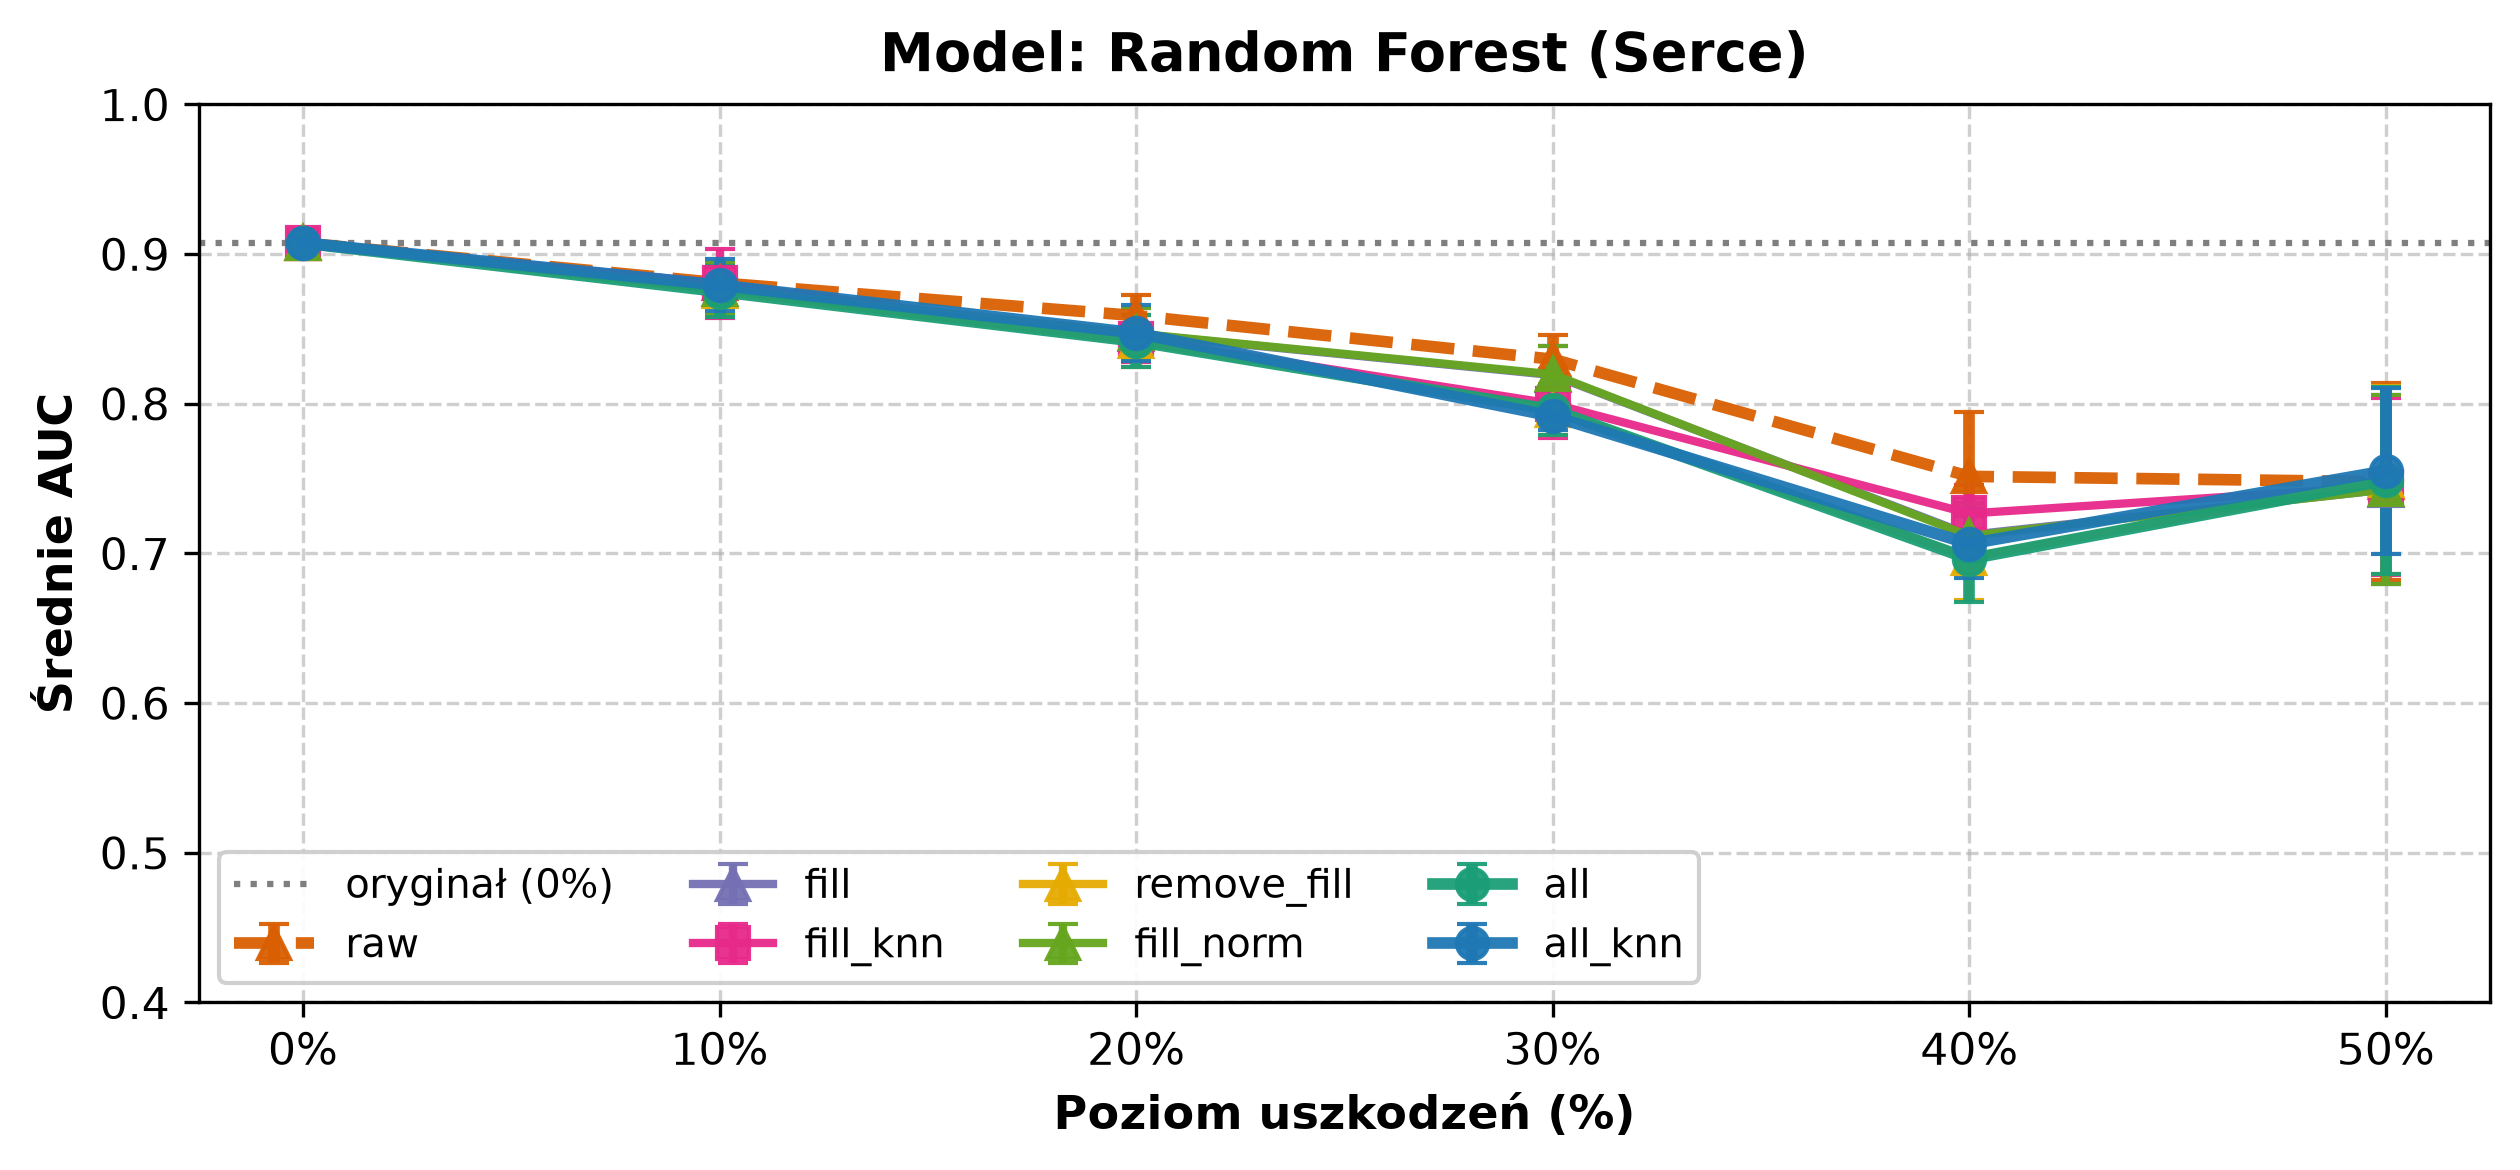
\includegraphics[width=\textwidth]{figures/Wykresy_Zaawansowane/1_Krzywe_Odpornosci/krzywa_serce_RF.png}
    \caption{Random Forest}
    \label{fig:odp_serce_rf}
\end{subfigure}
\vspace{0.25cm}
\begin{subfigure}[b]{0.92\textwidth}
    \centering
    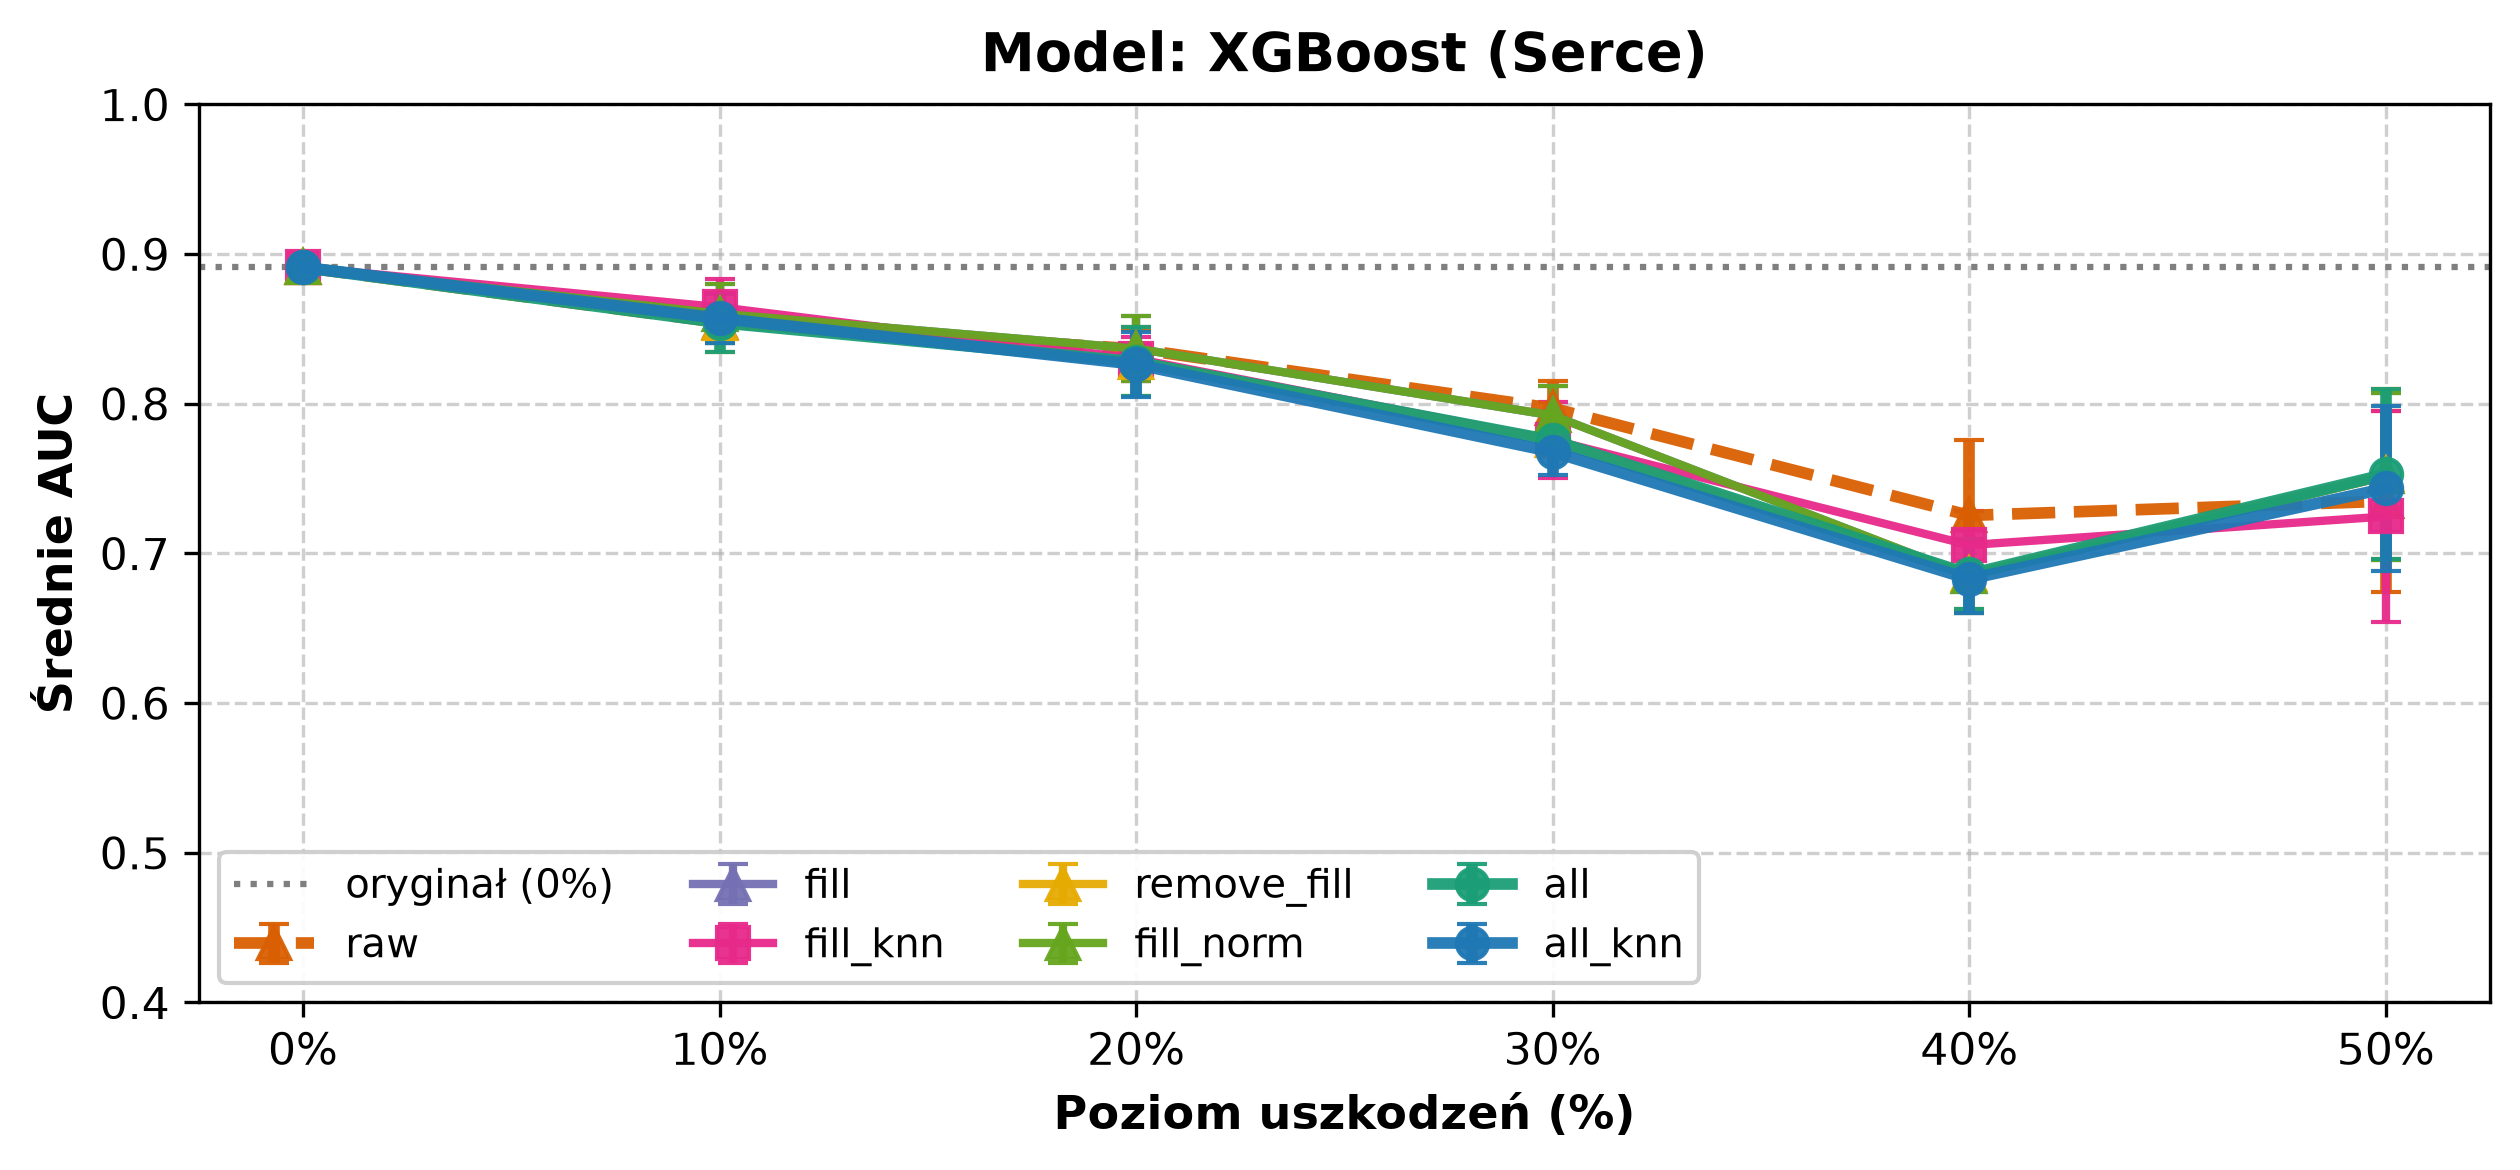
\includegraphics[width=\textwidth]{figures/Wykresy_Zaawansowane/1_Krzywe_Odpornosci/krzywa_serce_XGBoost.png}
    \caption{XGBoost}
    \label{fig:odp_serce_xgb}
\end{subfigure}
\caption{Krzywe odporności modeli zespołowych na zbiorze „Serce”}
\label{fig:odpornosc_serce_drzewa}
\end{figure}

\begin{figure}[H]
\centering
\begin{subfigure}[b]{0.92\textwidth}
    \centering
    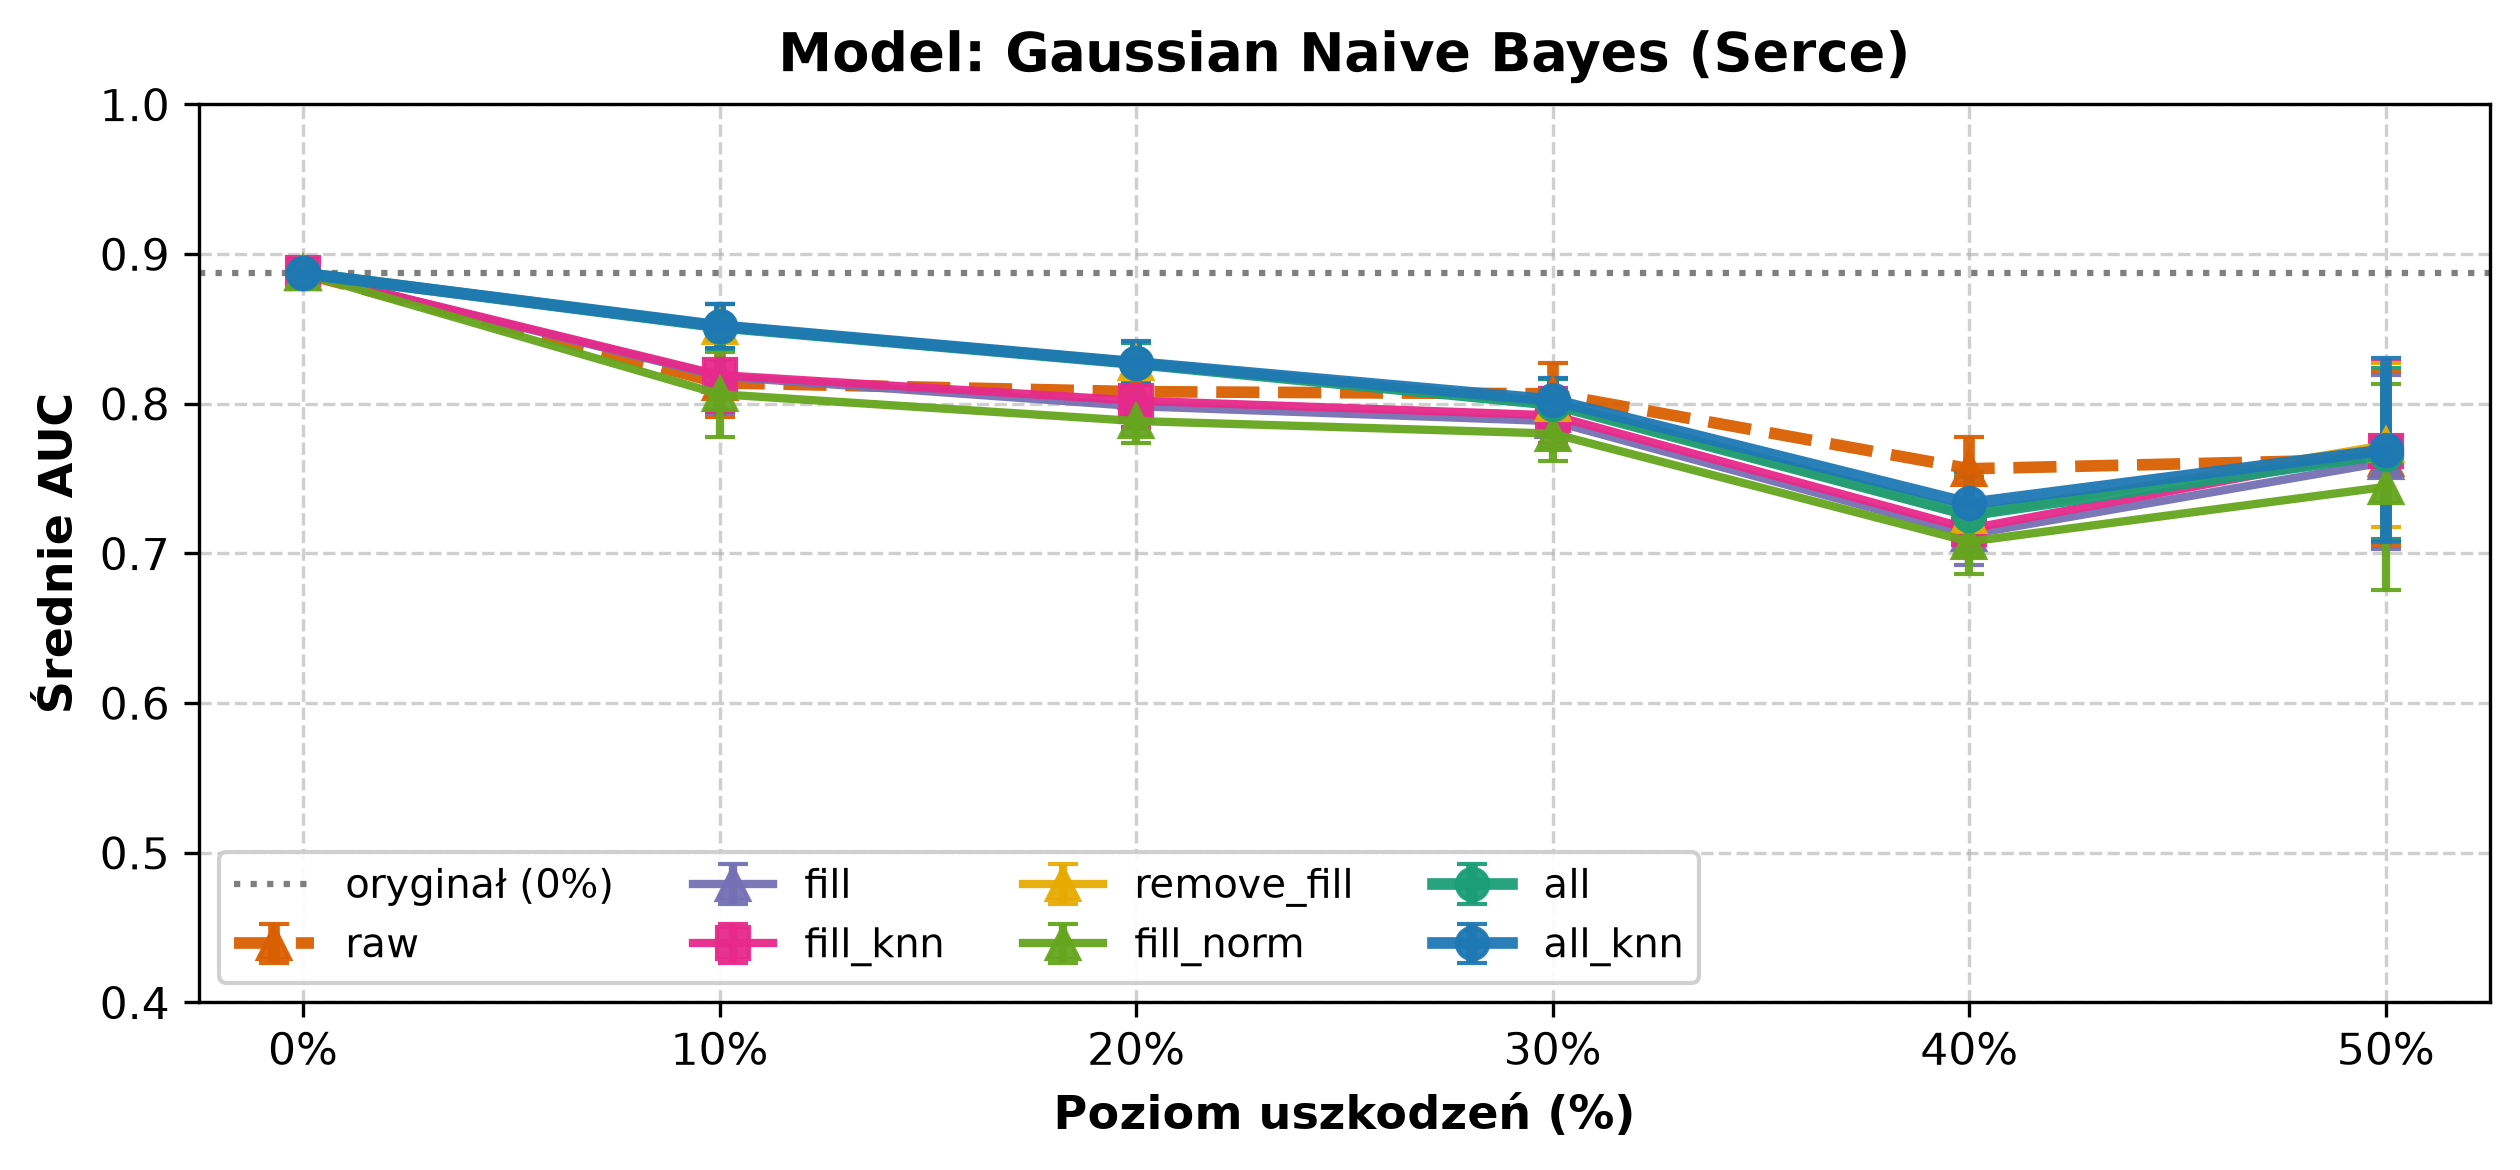
\includegraphics[width=\textwidth]{figures/Wykresy_Zaawansowane/1_Krzywe_Odpornosci/krzywa_serce_NB.png}
    \caption{Gaussian Naive Bayes}
    \label{fig:odp_serce_nb}
\end{subfigure}
\vspace{0.25cm}
\begin{subfigure}[b]{0.92\textwidth}
    \centering
    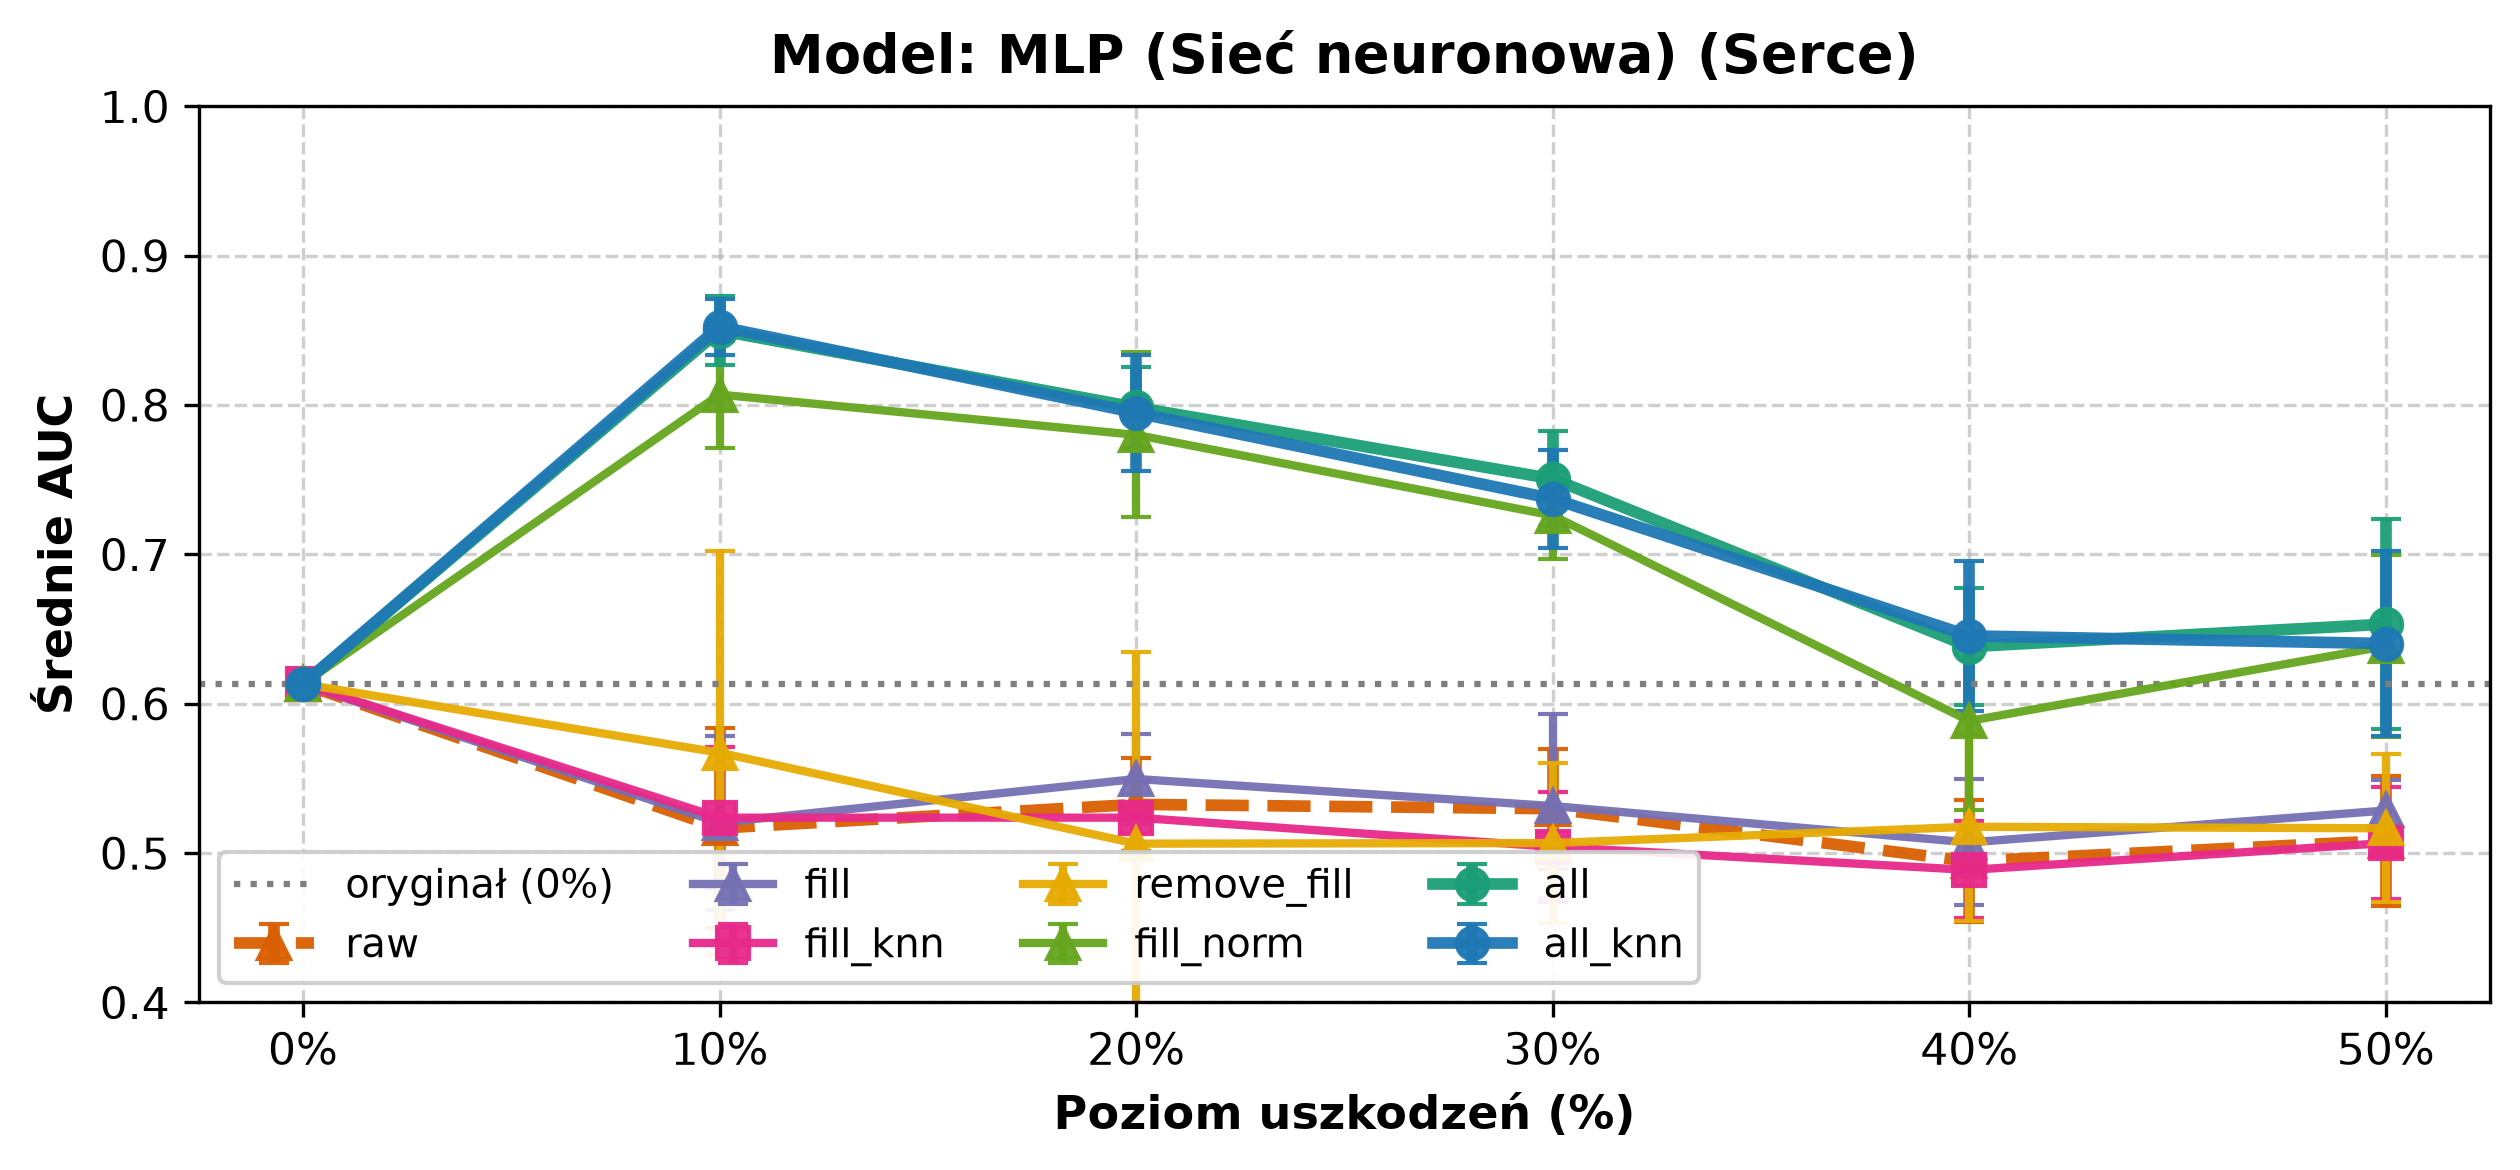
\includegraphics[width=\textwidth]{figures/Wykresy_Zaawansowane/1_Krzywe_Odpornosci/krzywa_serce_MLP.png}
    \caption{MLP (Sieć neuronowa)}
    \label{fig:odp_serce_mlp}
\end{subfigure}
\caption{Krzywe odporności klasyfikatora Bayesa i~sieci MLP na zbiorze „Serce”}
\label{fig:odpornosc_serce_inne}
\end{figure}

\begin{figure}[H]
\centering
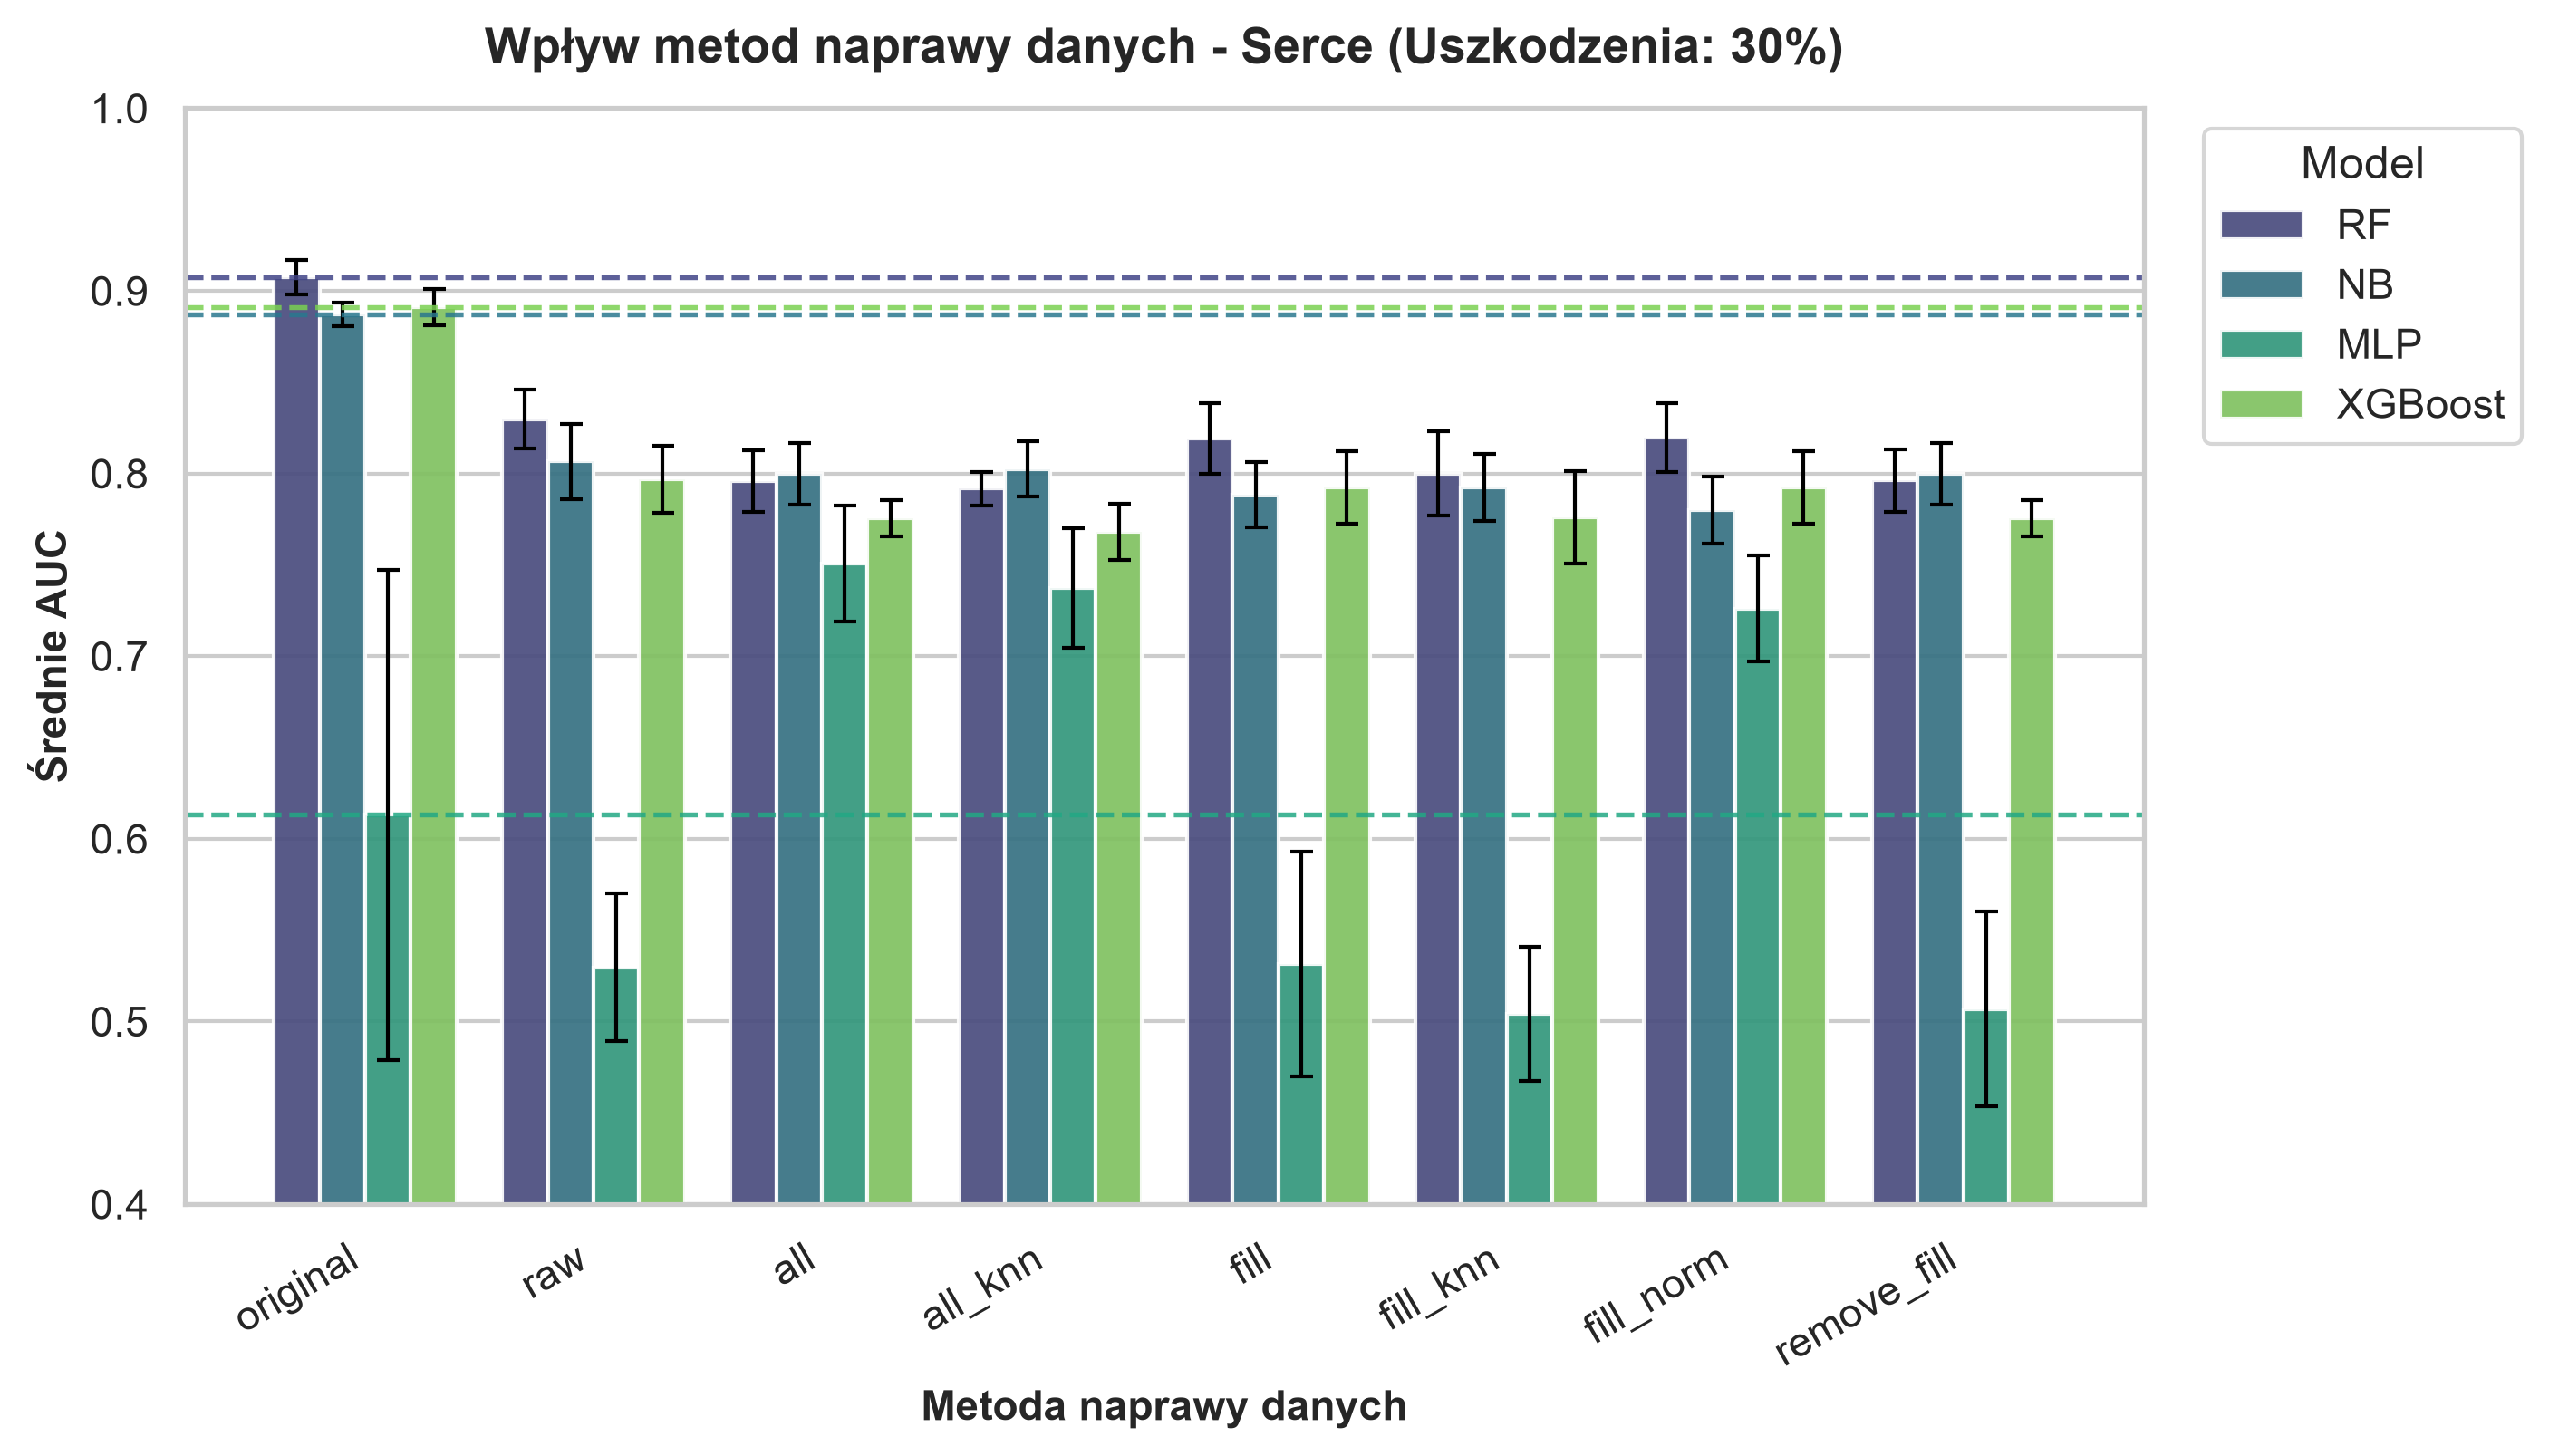
\includegraphics[width=0.95\textwidth]{figures/Wykresy_full/serce/serce_30proc.png}
\caption{Wpływ metod naprawy danych na jakość modeli na zbiorze „Serce” przy poziomie uszkodzeń 30\%}
\label{fig:slupkowy_serce_30}
\end{figure}

Analiza wyników na zbiorze kardiologicznym (Tabela~\ref{tab:wyniki_serce} oraz Rysunek~\ref{fig:slupkowy_serce_30}) wyraźnie uwidacznia, że prosta imputacja (\texttt{fill}) bez normalizacji jest niewystarczająca dla sieci MLP ($0{,}531$ przy $30\%$ uszkodzeń), podczas gdy połączenie filtracji outlierów, imputacji i~standaryzacji (\texttt{all}) podnosi jej jakość do poziomu $0{,}751$. Modele zespołowe (RF i~XGBoost) zachowują wysoką skuteczność ($\mathrm{AUC} > 0{,}75$) nawet przy $50\%$ uszkodzeń.

\subsection{Ocena na zbiorze „Diabetes” (Pima Indians Diabetes)}
Zbiór Indian Pima zawiera wyłącznie atrybuty ciągłe o~zróżnicowanych rozkładach. Zestawienie wartości $\overline{\mathrm{AUC}}$ przedstawiono w~tabeli~\ref{tab:wyniki_diabetes}. Ciągłe krzywe odporności oraz rozkład słupkowy przy uszkodzeniu $30\%$ zilustrowano na rysunkach~\ref{fig:odpornosc_diabetes} i~\ref{fig:slupkowy_diabetes_30}.

\begin{table}[H]
\centering
\caption{Wyniki $\overline{\mathrm{AUC}}$ na zbiorze „Diabetes” dla wszystkich poziomów degradacji}
\label{tab:wyniki_diabetes}
\vspace{0.2cm}
\resizebox{\textwidth}{!}{%
\begin{tabular}{llccccccc}
\toprule
\textbf{Model} & \textbf{Poziom} & \textbf{\texttt{raw}} & \textbf{\texttt{fill}} & \textbf{\texttt{fill\_knn}} & \textbf{\texttt{remove\_fill}} & \textbf{\texttt{fill\_norm}} & \textbf{\texttt{all}} & \textbf{\texttt{all\_knn}} \\
\midrule
\textbf{RF}      & 10\% & $0{,}7935$ & $0{,}8016$ & $0{,}7956$ & $\mathbf{0{,}8073}$ & $0{,}8016$ & $0{,}8072$ & $0{,}8004$ \\
                 & 20\% & $0{,}7606$ & $0{,}7698$ & $0{,}7667$ & $\mathbf{0{,}7823}$ & $0{,}7699$ & $0{,}7820$ & $0{,}7696$ \\
                 & 30\% & $0{,}7104$ & $0{,}7201$ & $0{,}7030$ & $\mathbf{0{,}7419}$ & $0{,}7202$ & $0{,}7418$ & $0{,}7188$ \\
                 & 40\% & $0{,}6550$ & $0{,}6777$ & $0{,}6645$ & $0{,}6849$ & $0{,}6774$ & $\mathbf{0{,}6850}$ & $0{,}6782$ \\
                 & 50\% & $\mathbf{0{,}6345}$ & $0{,}6306$ & $0{,}6202$ & $0{,}6319$ & $0{,}6312$ & $0{,}6322$ & $0{,}6043$ \\
\midrule
\textbf{XGBoost} & 10\% & $0{,}7887$ & $0{,}7903$ & $0{,}7901$ & $\mathbf{0{,}7947}$ & $0{,}7903$ & $\mathbf{0{,}7947}$ & $0{,}7904$ \\
                 & 20\% & $0{,}7677$ & $0{,}7693$ & $0{,}7669$ & $\mathbf{0{,}7756}$ & $0{,}7693$ & $\mathbf{0{,}7756}$ & $0{,}7597$ \\
                 & 30\% & $0{,}7303$ & $0{,}7344$ & $0{,}7091$ & $\mathbf{0{,}7433}$ & $0{,}7344$ & $\mathbf{0{,}7433}$ & $0{,}7117$ \\
                 & 40\% & $0{,}6696$ & $0{,}6865$ & $0{,}6691$ & $\mathbf{0{,}6986}$ & $0{,}6865$ & $\mathbf{0{,}6986}$ & $0{,}6649$ \\
                 & 50\% & $0{,}6566$ & $0{,}6576$ & $0{,}6249$ & $\mathbf{0{,}6600}$ & $0{,}6576$ & $\mathbf{0{,}6600}$ & $0{,}6153$ \\
\midrule
\textbf{NB}      & 10\% & $0{,}5162$ & $0{,}5130$ & $0{,}5035$ & $0{,}7868$ & $0{,}5130$ & $0{,}7868$ & $\mathbf{0{,}7888}$ \\
                 & 20\% & $0{,}5055$ & $0{,}4993$ & $0{,}5120$ & $\mathbf{0{,}7682}$ & $0{,}4993$ & $\mathbf{0{,}7682}$ & $0{,}7674$ \\
                 & 30\% & $0{,}5154$ & $0{,}5069$ & $0{,}5217$ & $0{,}7122$ & $0{,}5069$ & $0{,}7122$ & $\mathbf{0{,}7221}$ \\
                 & 40\% & $0{,}5507$ & $0{,}5462$ & $0{,}5521$ & $0{,}6488$ & $0{,}5462$ & $0{,}6488$ & $\mathbf{0{,}6674}$ \\
                 & 50\% & $0{,}5245$ & $0{,}5208$ & $0{,}5295$ & $0{,}5187$ & $0{,}5208$ & $0{,}5187$ & $\mathbf{0{,}5322}$ \\
\midrule
\textbf{MLP}     & 10\% & $0{,}4807$ & $0{,}4788$ & $0{,}4804$ & $0{,}5905$ & $0{,}5245$ & $\mathbf{0{,}7719}$ & $0{,}7686$ \\
                 & 20\% & $0{,}4969$ & $0{,}4886$ & $0{,}4944$ & $0{,}5484$ & $0{,}4912$ & $\mathbf{0{,}7468}$ & $0{,}7387$ \\
                 & 30\% & $0{,}4953$ & $0{,}4976$ & $0{,}5088$ & $0{,}5512$ & $0{,}5156$ & $\mathbf{0{,}7157}$ & $0{,}6852$ \\
                 & 40\% & $0{,}4924$ & $0{,}4915$ & $0{,}4918$ & $0{,}5297$ & $0{,}4828$ & $\mathbf{0{,}6454}$ & $0{,}6095$ \\
                 & 50\% & $0{,}4850$ & $0{,}4954$ & $0{,}4964$ & $0{,}4990$ & $0{,}4996$ & $0{,}5014$ & $\mathbf{0{,}5110}$ \\
\bottomrule
\end{tabular}%
}
\end{table}

\begin{figure}[H]
\centering
\begin{subfigure}[b]{0.92\textwidth}
    \centering
    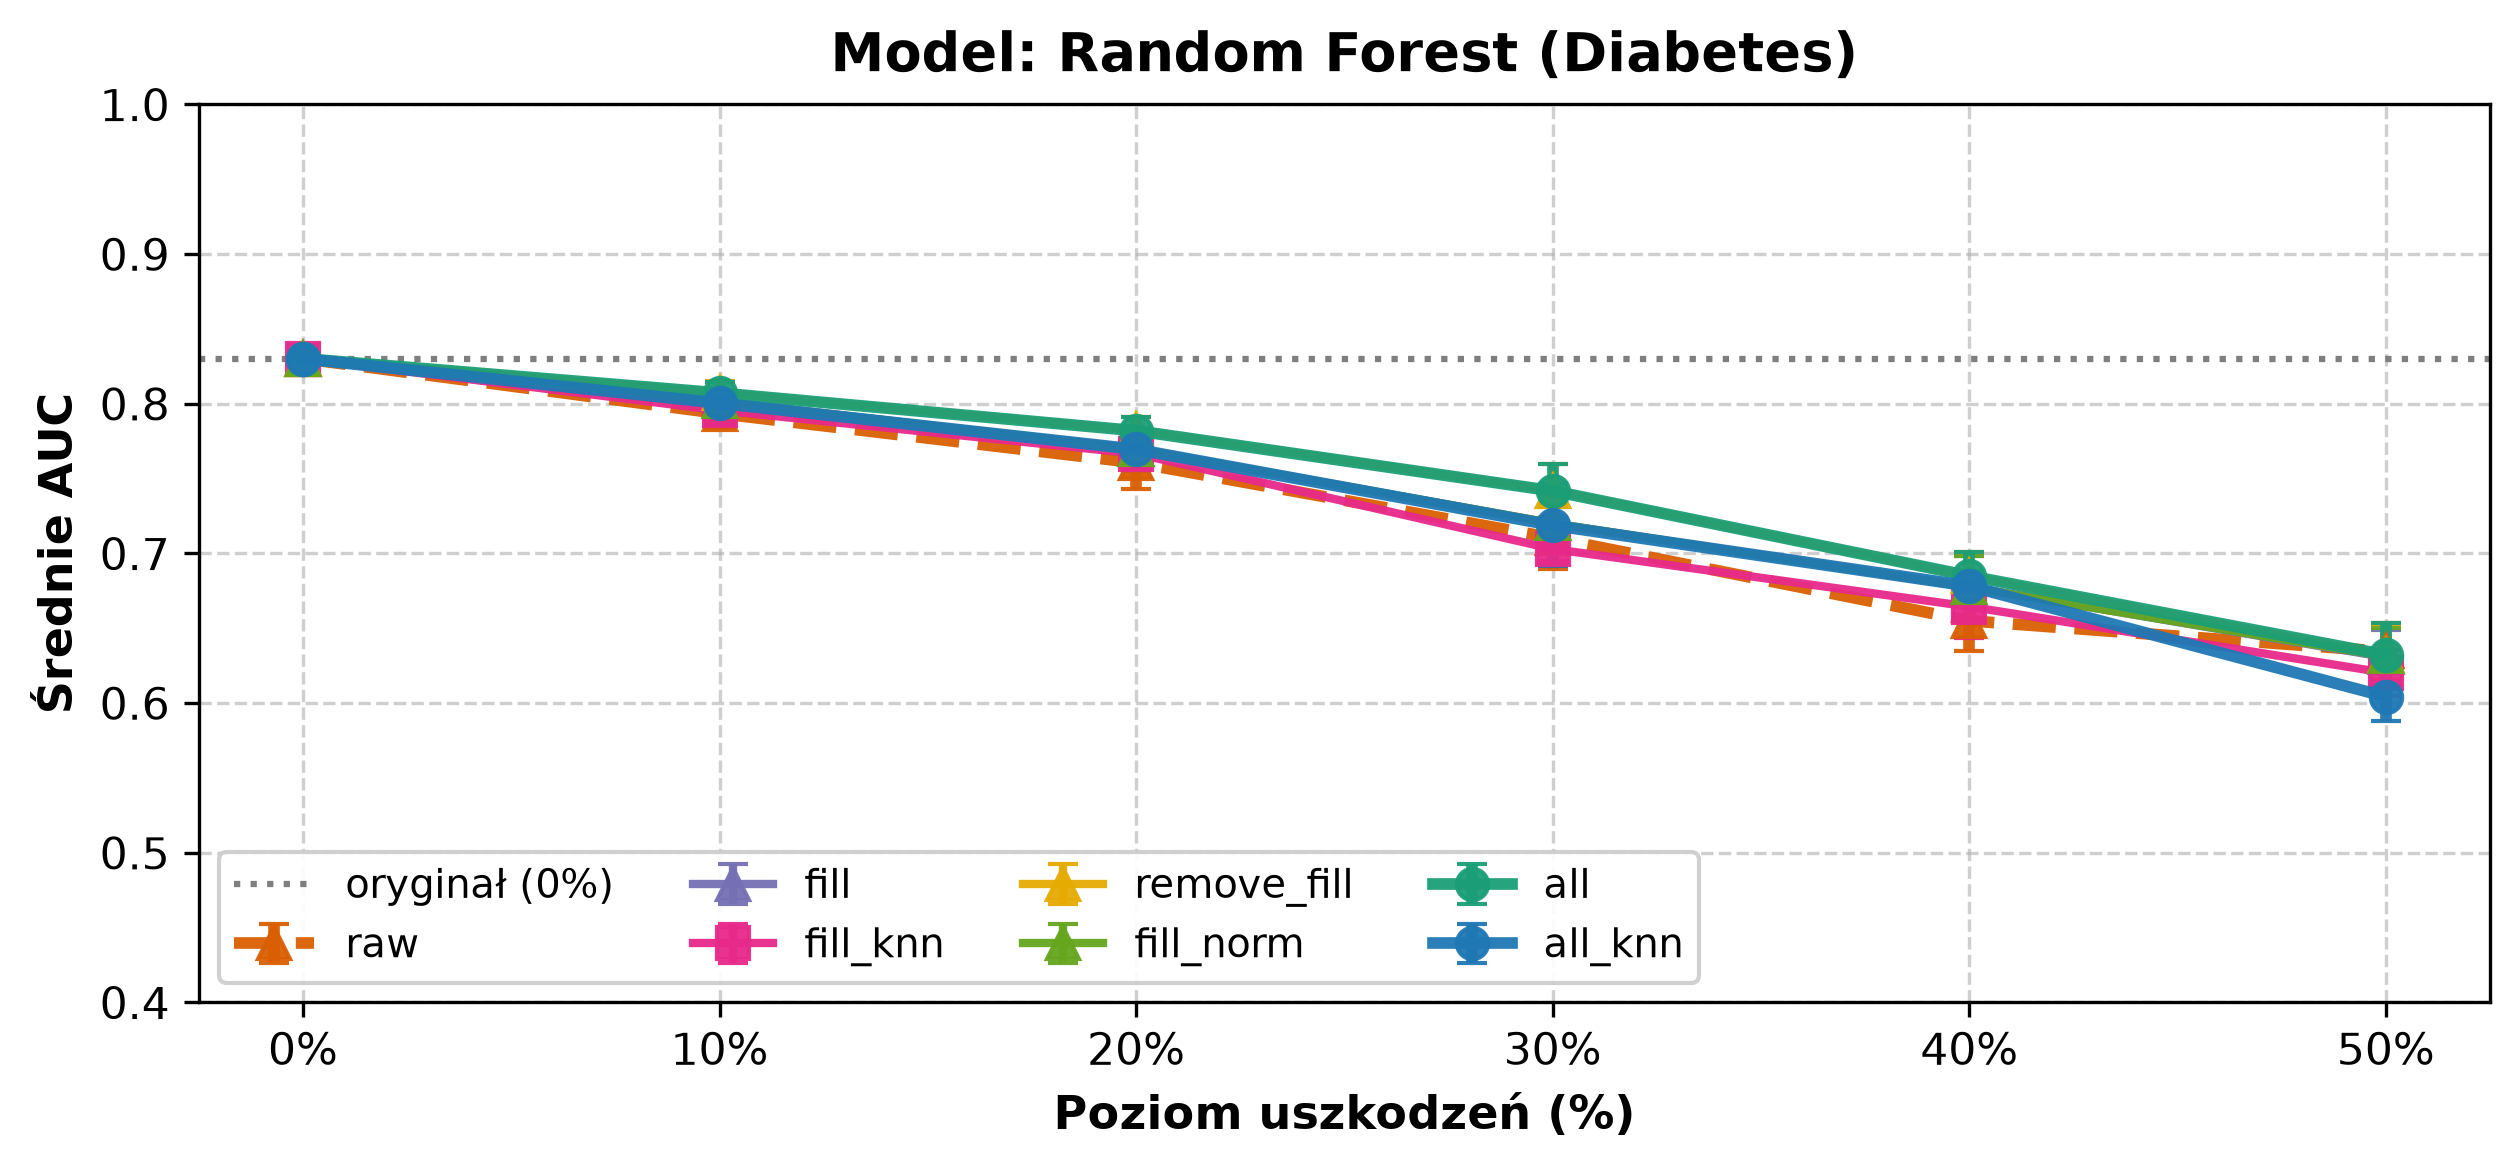
\includegraphics[width=\textwidth]{figures/Wykresy_Zaawansowane/1_Krzywe_Odpornosci/krzywa_diabetes_RF.png}
    \caption{Random Forest}
    \label{fig:odp_diab_rf}
\end{subfigure}
\vspace{0.25cm}
\begin{subfigure}[b]{0.92\textwidth}
    \centering
    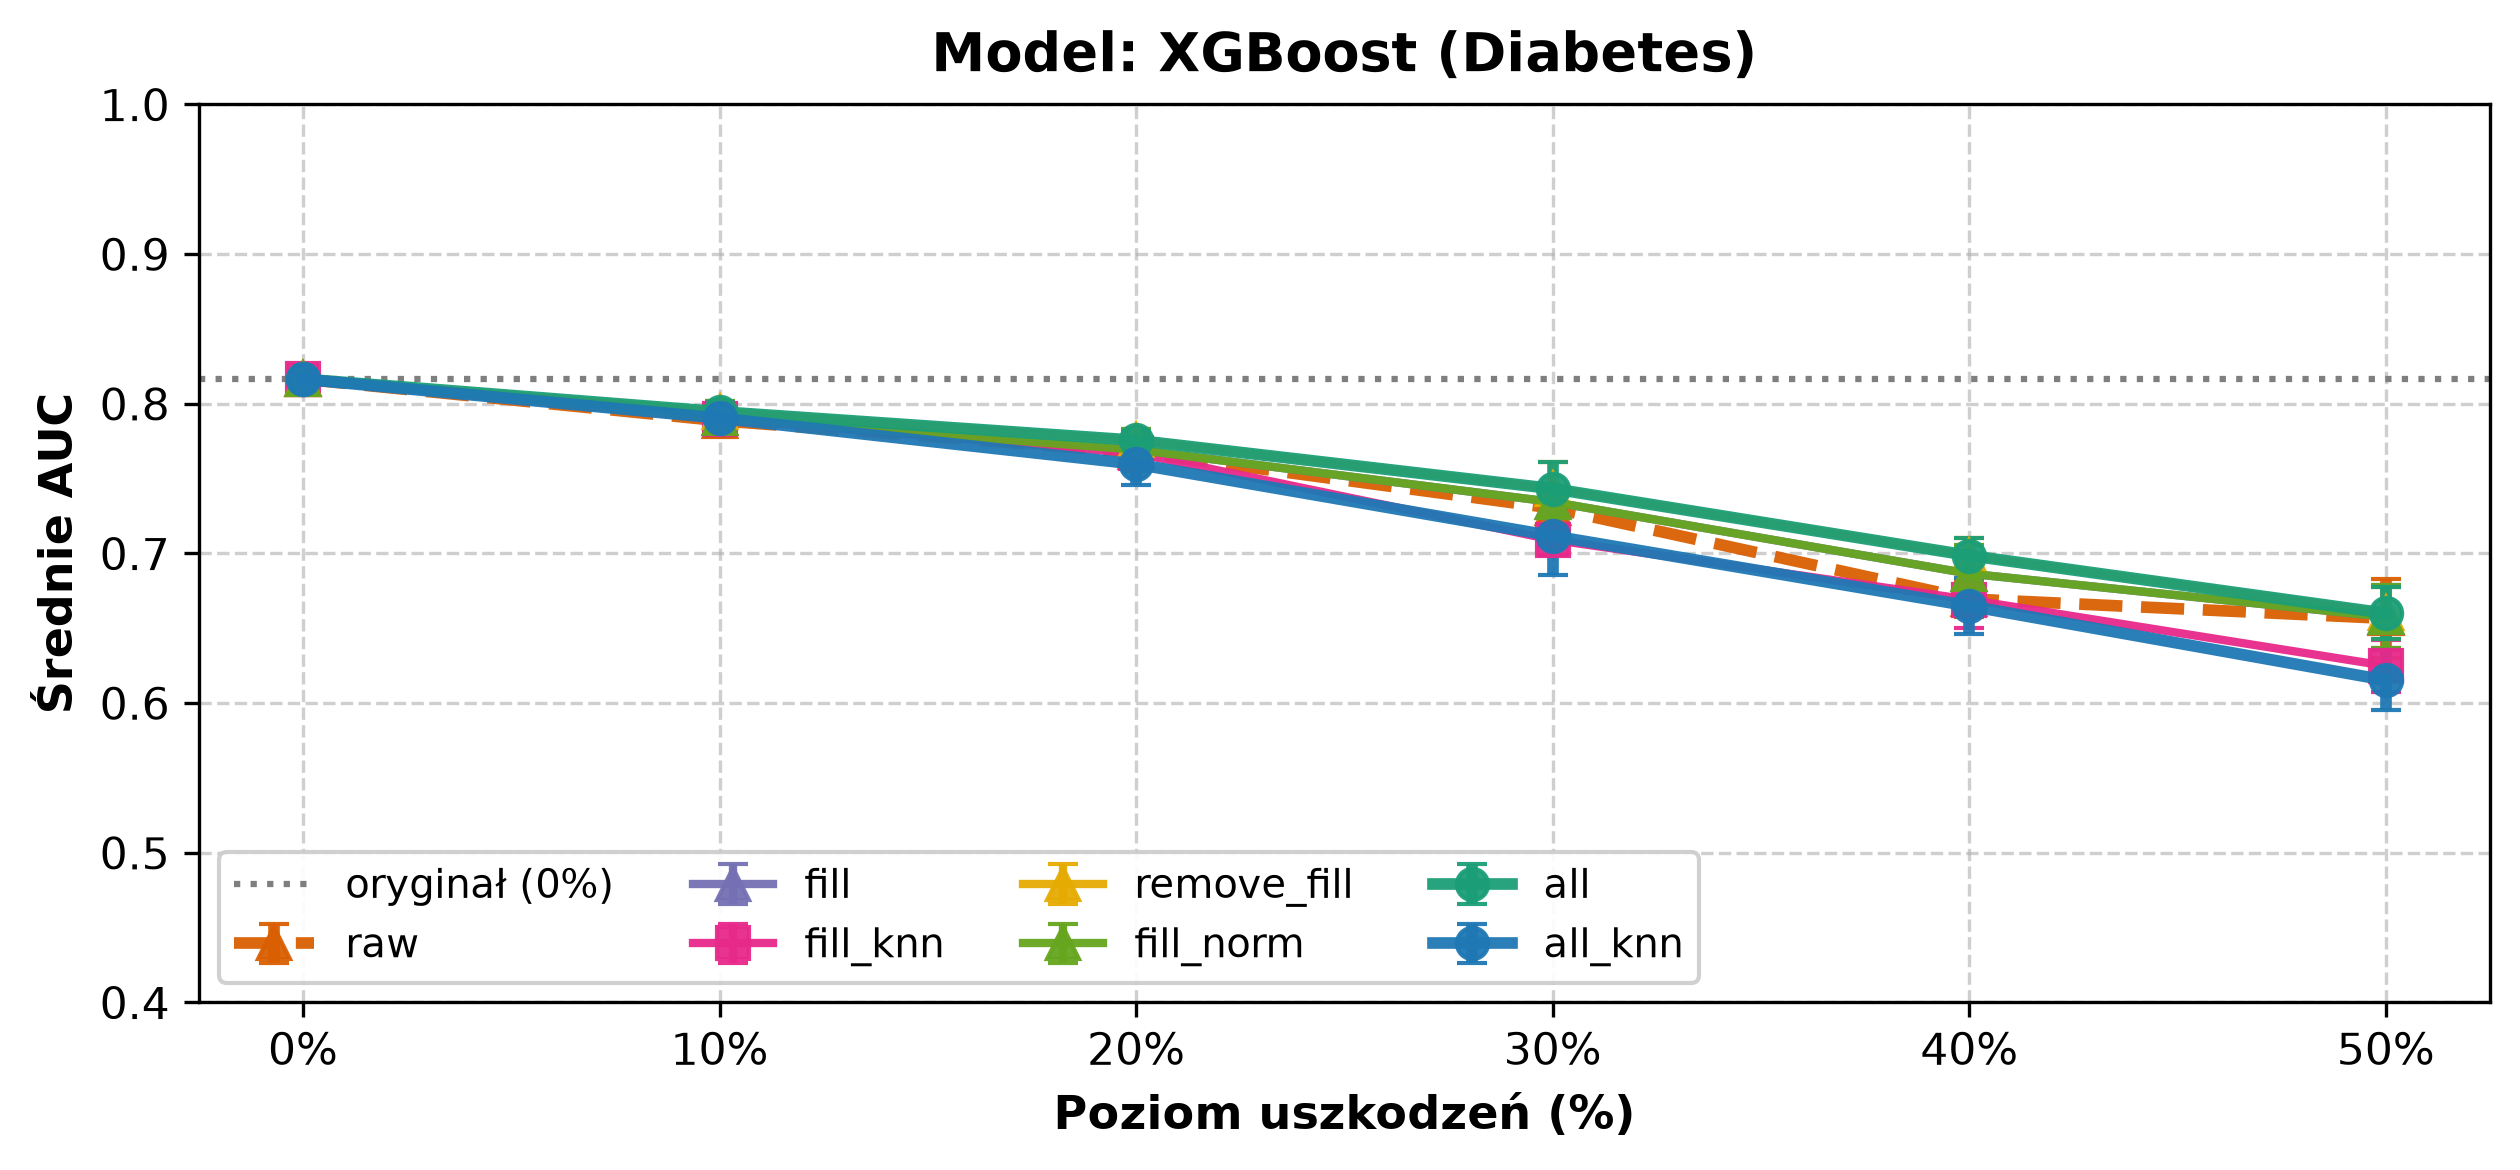
\includegraphics[width=\textwidth]{figures/Wykresy_Zaawansowane/1_Krzywe_Odpornosci/krzywa_diabetes_XGBoost.png}
    \caption{XGBoost}
    \label{fig:odp_diab_xgb}
\end{subfigure}
\caption{Krzywe odporności modeli zespołowych na zbiorze „Diabetes”}
\label{fig:odpornosc_diabetes_drzewa}
\end{figure}

\begin{figure}[H]
\centering
\begin{subfigure}[b]{0.92\textwidth}
    \centering
    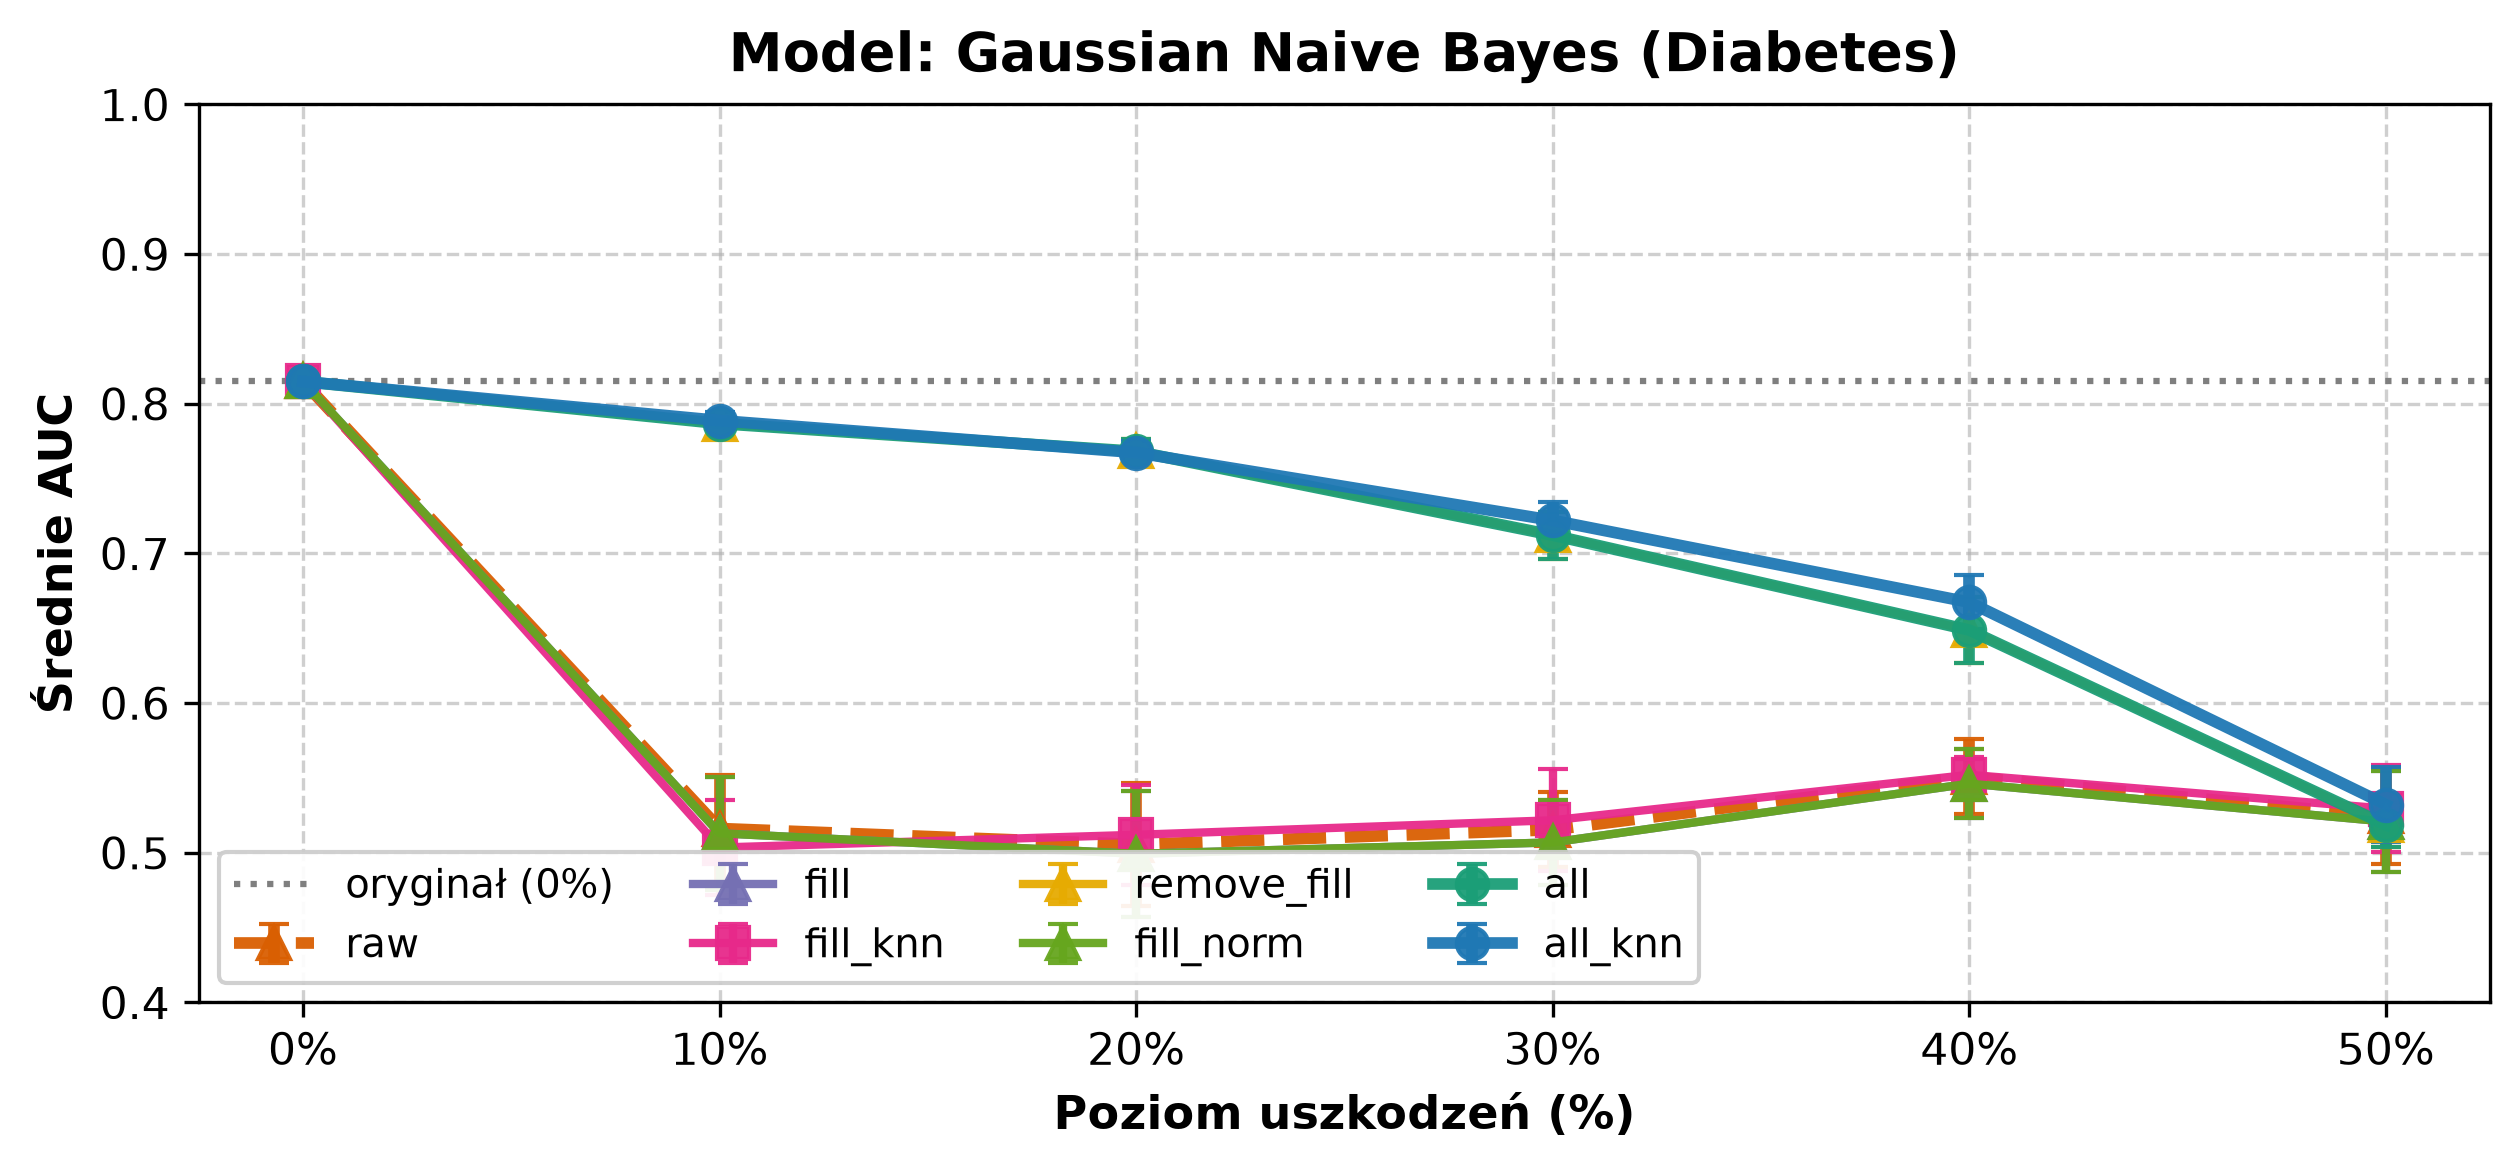
\includegraphics[width=\textwidth]{figures/Wykresy_Zaawansowane/1_Krzywe_Odpornosci/krzywa_diabetes_NB.png}
    \caption{Gaussian Naive Bayes}
    \label{fig:odp_diab_nb}
\end{subfigure}
\vspace{0.25cm}
\begin{subfigure}[b]{0.92\textwidth}
    \centering
    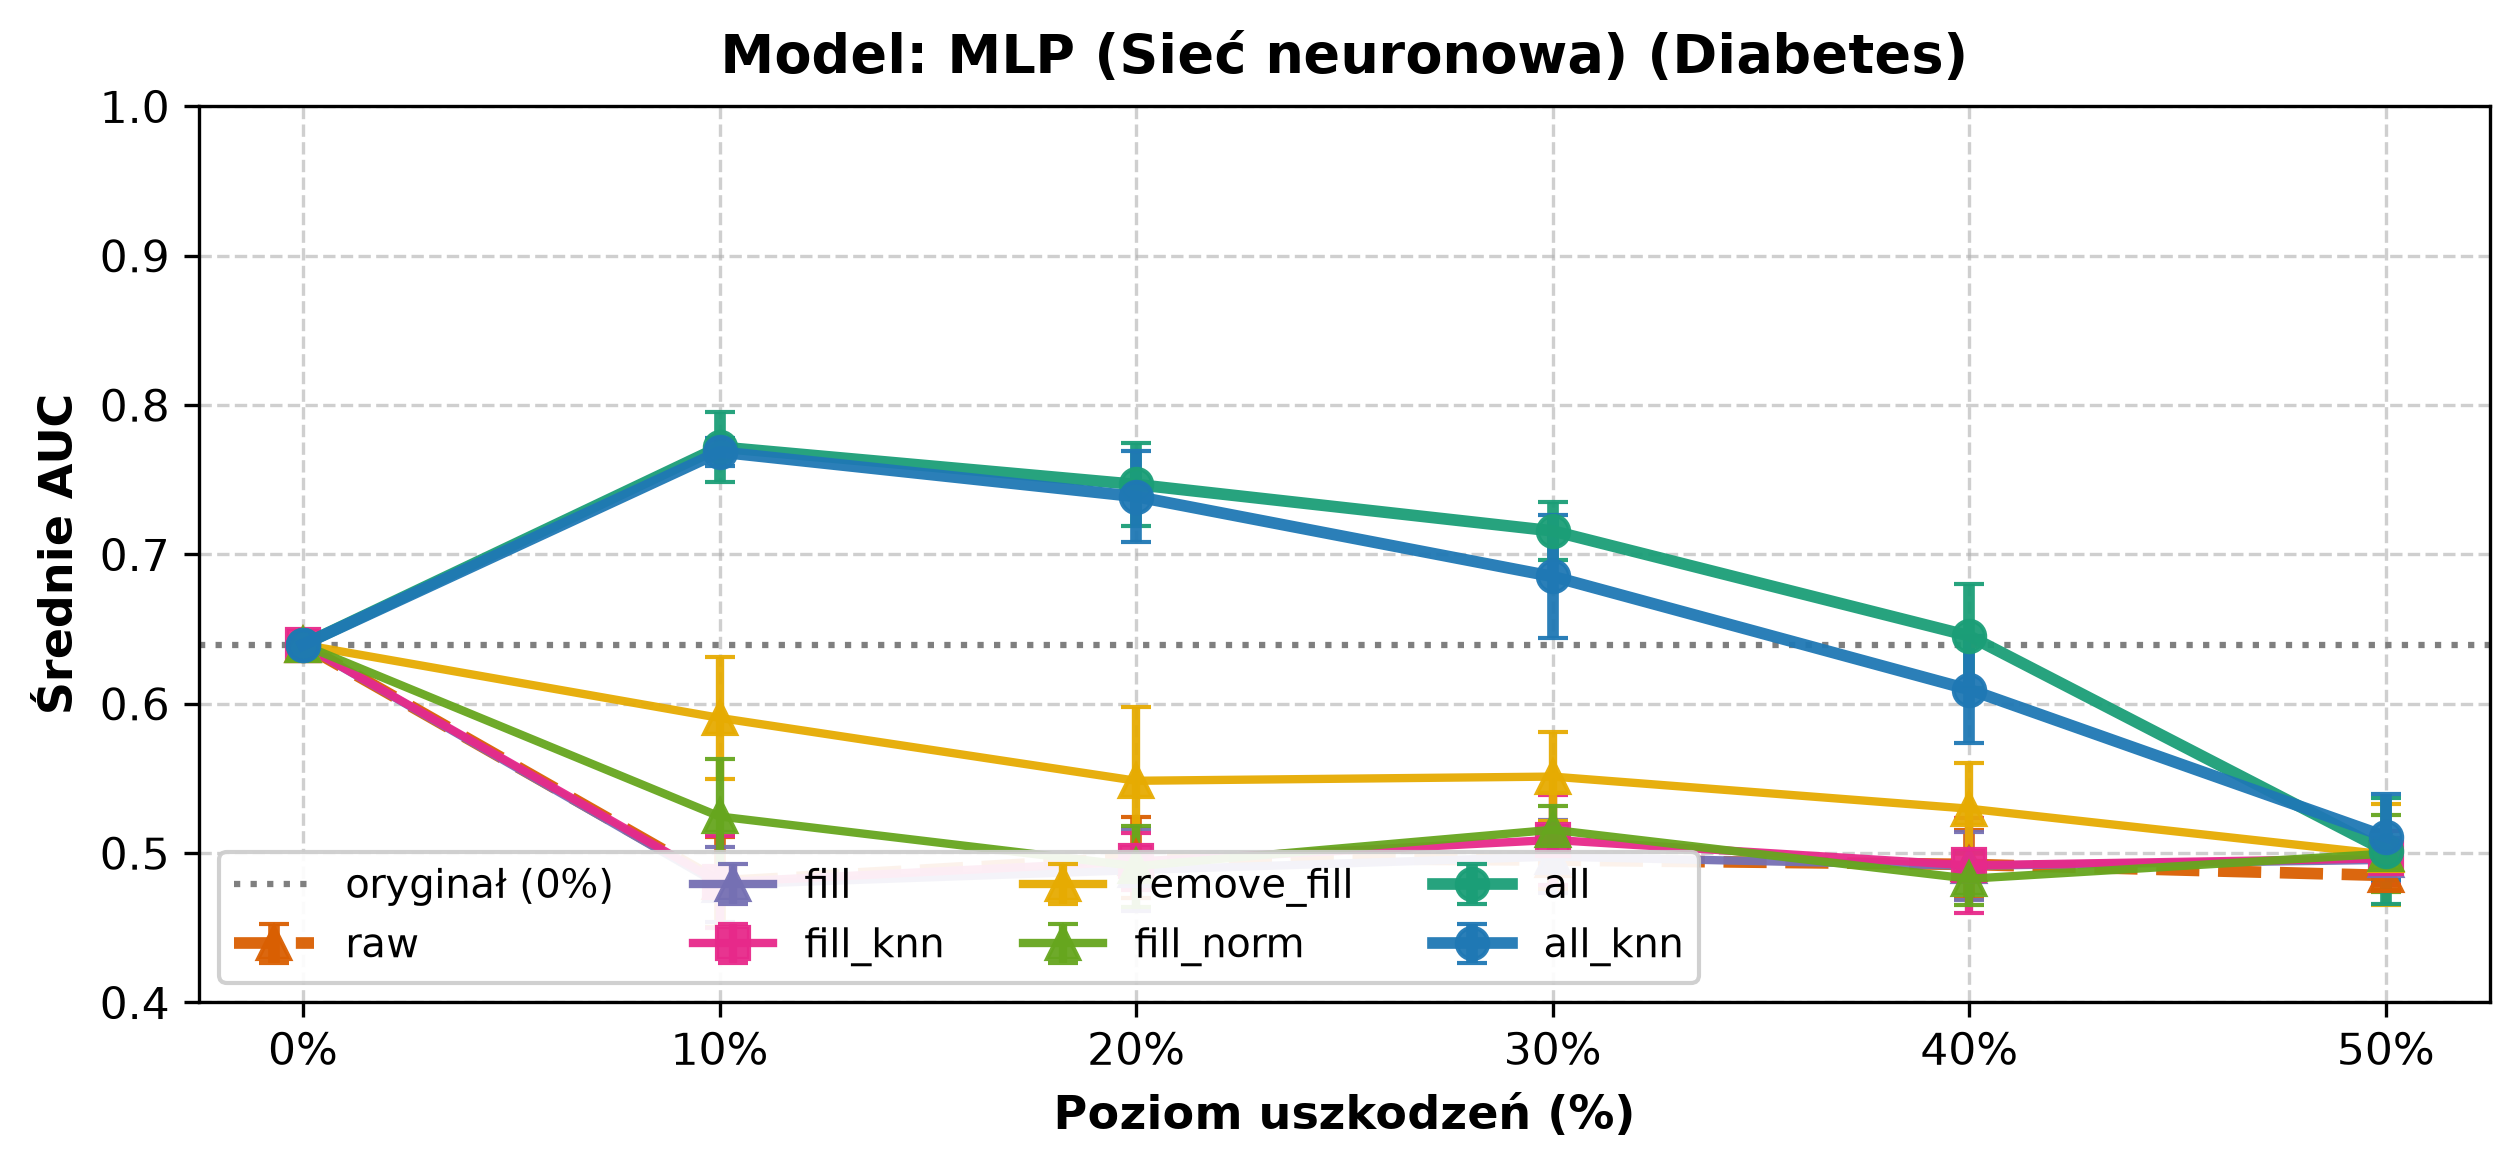
\includegraphics[width=\textwidth]{figures/Wykresy_Zaawansowane/1_Krzywe_Odpornosci/krzywa_diabetes_MLP.png}
    \caption{MLP (Sieć neuronowa)}
    \label{fig:odp_diab_mlp}
\end{subfigure}
\caption{Krzywe odporności klasyfikatora Bayesa i~sieci MLP na zbiorze „Diabetes”}
\label{fig:odpornosc_diabetes_inne}
\end{figure}

\begin{figure}[H]
\centering
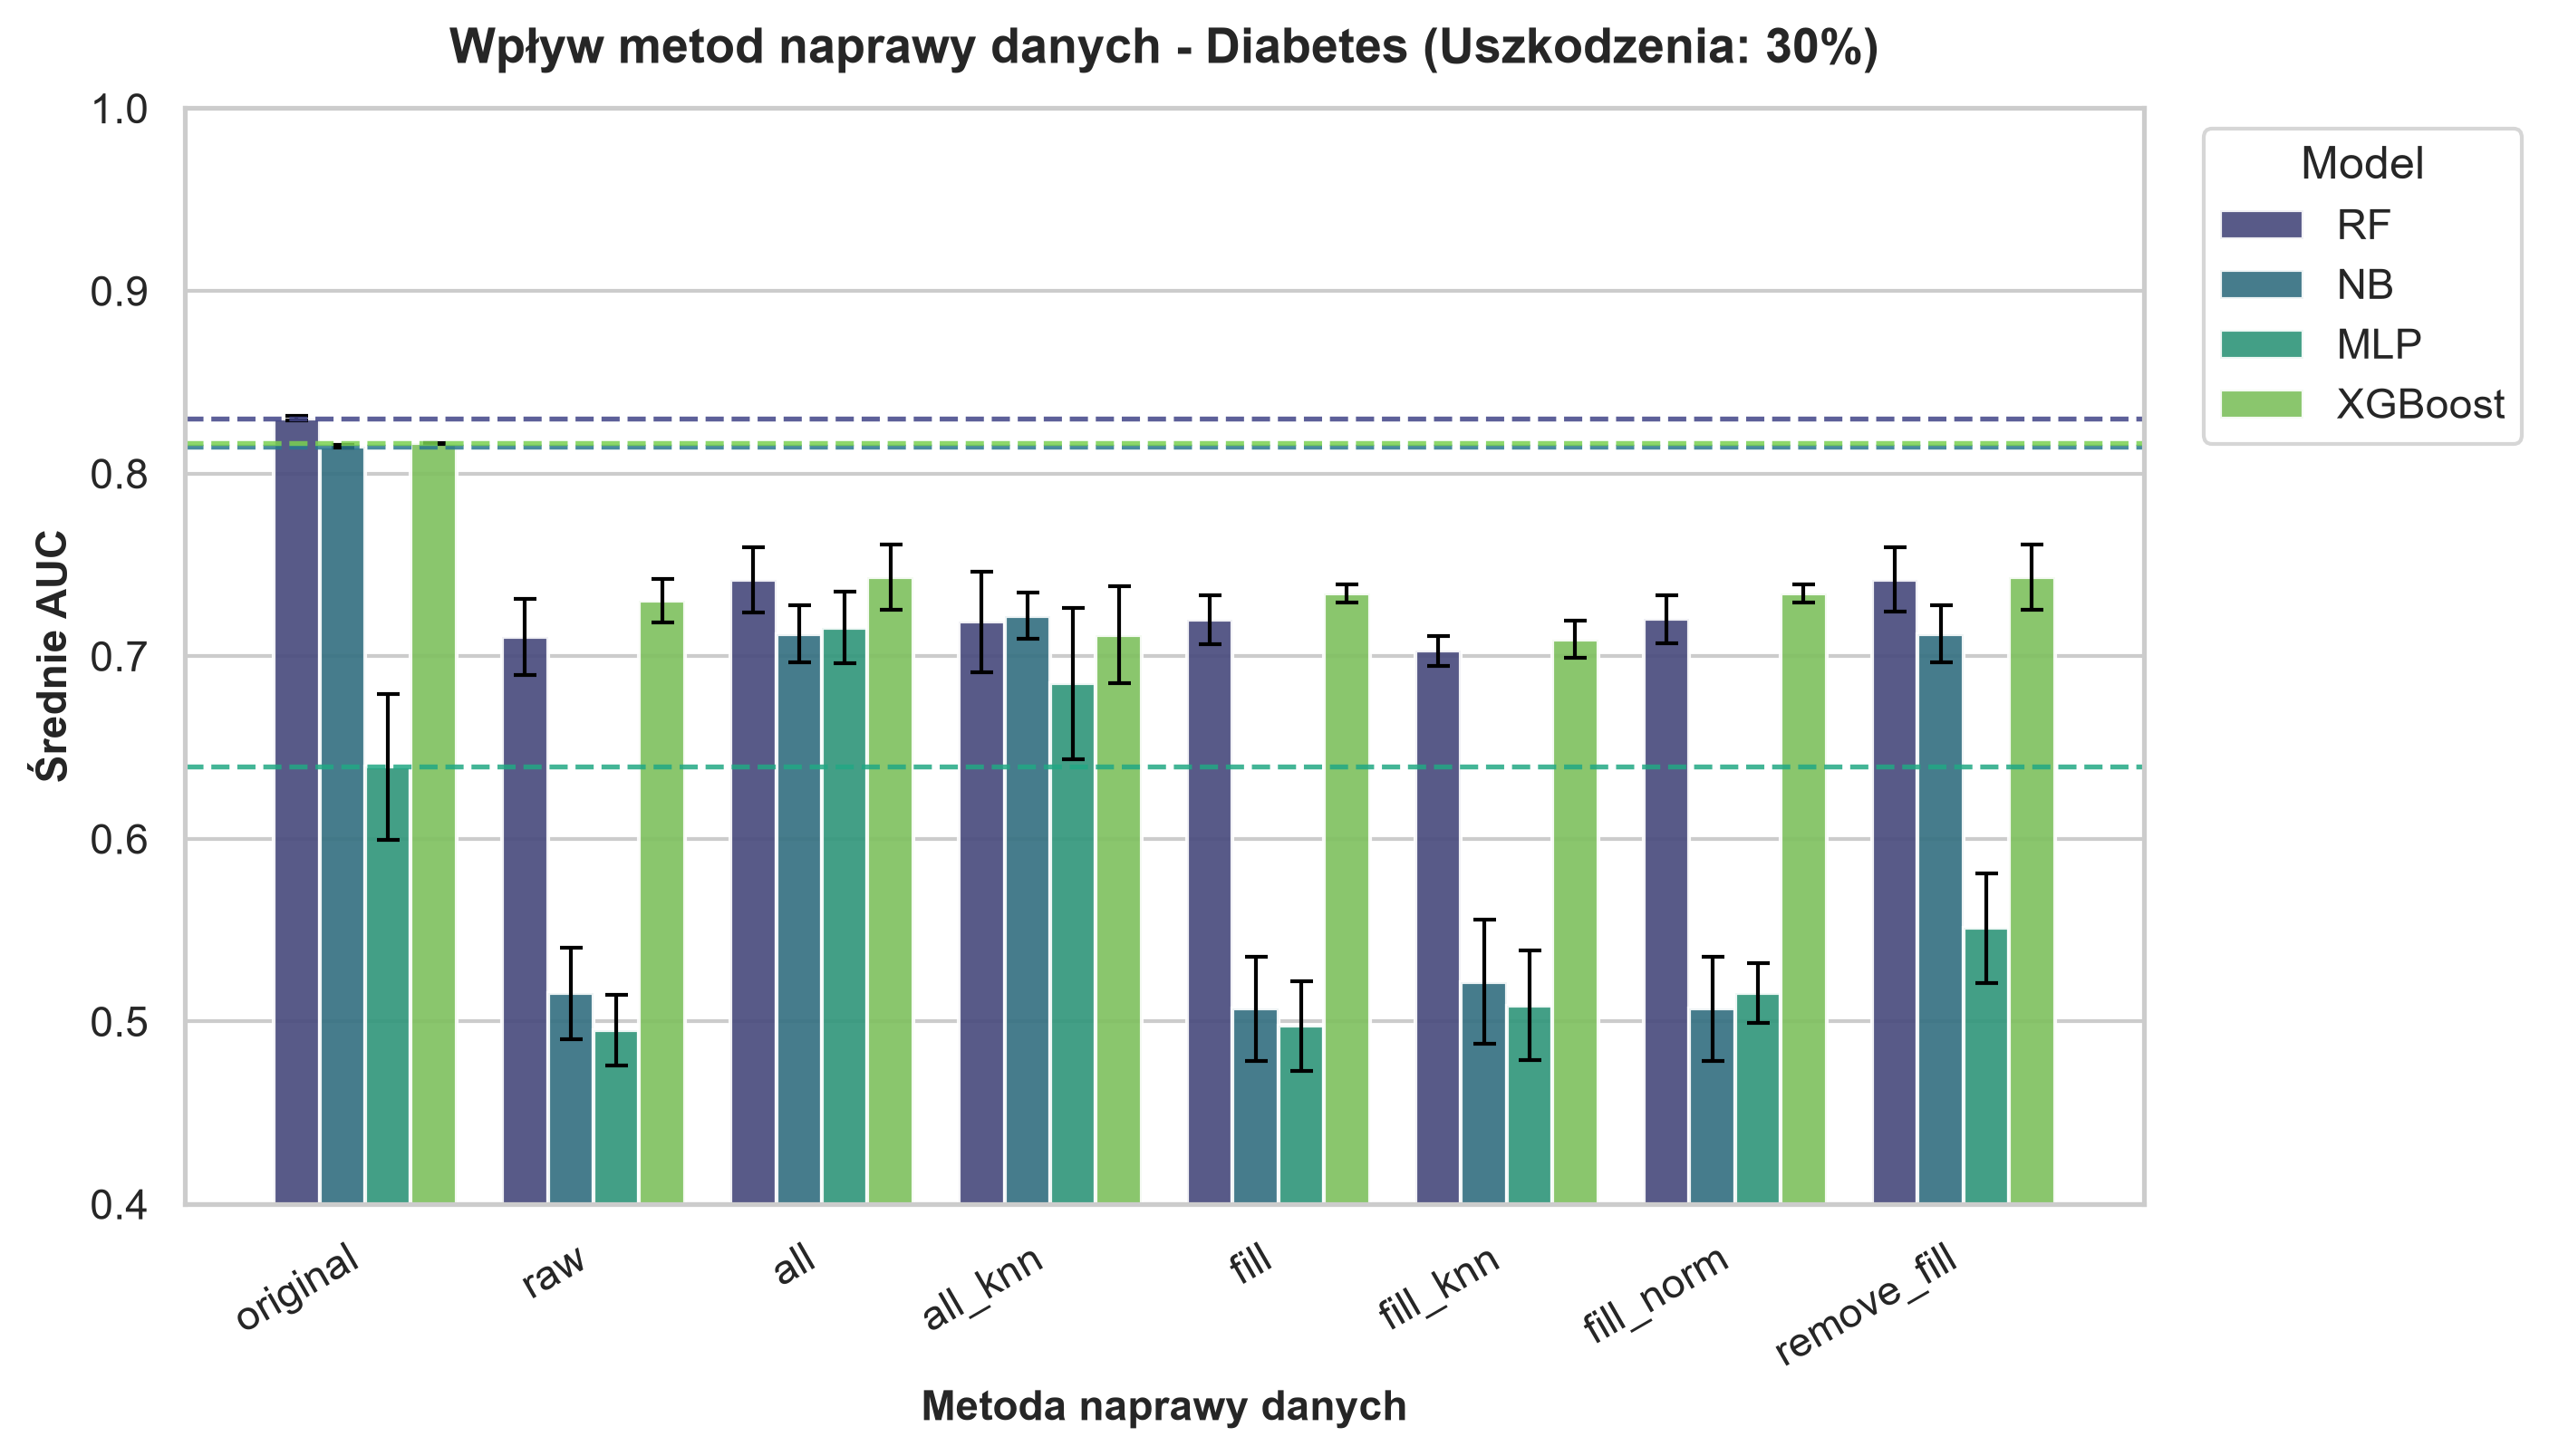
\includegraphics[width=0.95\textwidth]{figures/Wykresy_full/diabetes/diabetes_30proc.png}
\caption{Porównanie skuteczności metod czyszczenia na zbiorze „Diabetes” przy uszkodzeniu 30\%}
\label{fig:slupkowy_diabetes_30}
\end{figure}

W~zbiorze „Diabetes” (Tabela~\ref{tab:wyniki_diabetes}) brak normalizacji i~obecność ekstremalnych wartości odstających prowadzi do całkowitej degradacji sieci MLP ($\mathrm{AUC} \approx 0{,}485$ przy $50\%$ uszkodzeń, co odpowiada klasyfikatorowi losowemu). Wdrożenie potoku \textit{all} przywraca stabilność optymalizacji gradientowej, podnosząc skuteczność sieci do poziomu $0{,}716$ przy $30\%$ uszkodzeń. Z~kolei algorytm GaussianNB na danych nieoczyszczonych traci skuteczność z~$0{,}815$ do $0{,}515$ na skutek zaburzenia estymacji wariancji przez błędy grube, zyskując aż do $0{,}787$ po odfiltrowaniu anomalii potokiem \textit{remove\_fill} lub \textit{all}.

\subsection{Ocena na zbiorze „Rezygnacje” (Customer Churn)}
Zbiór telekomunikacyjny charakteryzuje się dużą próbą ($N=3333$) i~dominacją atrybutów bilingowych. Szczegółowe wartości $\overline{\mathrm{AUC}}$ w~zależności od metody i~poziomu degradacji zestawiono w~tabeli~\ref{tab:wyniki_rezygnacje}. Odpowiednie wykresy przedstawiono na rysunkach~\ref{fig:odpornosc_rezygnacje_drzewa}, \ref{fig:odpornosc_rezygnacje_inne} i~\ref{fig:slupkowy_rezygnacje_30}.

\begin{table}[H]
\centering
\caption{Wyniki $\overline{\mathrm{AUC}}$ na zbiorze „Rezygnacje” dla wszystkich poziomów degradacji}
\label{tab:wyniki_rezygnacje}
\vspace{0.2cm}
\resizebox{\textwidth}{!}{%
\begin{tabular}{llccccccc}
\toprule
\textbf{Model} & \textbf{Poziom} & \textbf{\texttt{raw}} & \textbf{\texttt{fill}} & \textbf{\texttt{fill\_knn}} & \textbf{\texttt{remove\_fill}} & \textbf{\texttt{fill\_norm}} & \textbf{\texttt{all}} & \textbf{\texttt{all\_knn}} \\
\midrule
\textbf{RF}      & 10\% & $\mathbf{0{,}8577}$ & $0{,}8543$ & $0{,}8557$ & $0{,}8349$ & $0{,}8541$ & $0{,}8349$ & $0{,}8367$ \\
                 & 20\% & $\mathbf{0{,}8122}$ & $0{,}8062$ & $0{,}7983$ & $0{,}8080$ & $0{,}8062$ & $0{,}8078$ & $0{,}8111$ \\
                 & 30\% & $0{,}7462$ & $0{,}7471$ & $0{,}7231$ & $0{,}7599$ & $0{,}7470$ & $0{,}7599$ & $\mathbf{0{,}7628}$ \\
                 & 40\% & $0{,}7011$ & $0{,}7016$ & $0{,}6698$ & $\mathbf{0{,}7082}$ & $0{,}7016$ & $\mathbf{0{,}7082}$ & $0{,}7050$ \\
                 & 50\% & $0{,}6532$ & $0{,}6560$ & $0{,}6206$ & $\mathbf{0{,}6589}$ & $0{,}6559$ & $0{,}6586$ & $0{,}6271$ \\
\midrule
\textbf{XGBoost} & 10\% & $\mathbf{0{,}8623}$ & $0{,}8584$ & $0{,}8580$ & $0{,}8425$ & $0{,}8584$ & $0{,}8425$ & $0{,}8432$ \\
                 & 20\% & $\mathbf{0{,}8183}$ & $0{,}8125$ & $0{,}8118$ & $0{,}8171$ & $0{,}8125$ & $0{,}8171$ & $0{,}8147$ \\
                 & 30\% & $0{,}7667$ & $0{,}7652$ & $0{,}7512$ & $\mathbf{0{,}7763}$ & $0{,}7652$ & $\mathbf{0{,}7763}$ & $0{,}7693$ \\
                 & 40\% & $\mathbf{0{,}7300}$ & $0{,}7211$ & $0{,}7060$ & $0{,}7276$ & $0{,}7211$ & $0{,}7276$ & $0{,}7044$ \\
                 & 50\% & $0{,}6890$ & $\mathbf{0{,}6932}$ & $0{,}6486$ & $0{,}6853$ & $\mathbf{0{,}6932}$ & $0{,}6853$ & $0{,}6448$ \\
\midrule
\textbf{NB}      & 10\% & $0{,}5999$ & $0{,}6038$ & $0{,}6049$ & $0{,}7684$ & $0{,}5884$ & $0{,}7684$ & $\mathbf{0{,}7691}$ \\
                 & 20\% & $0{,}5965$ & $0{,}5961$ & $0{,}5974$ & $\mathbf{0{,}7710}$ & $0{,}5775$ & $\mathbf{0{,}7710}$ & $0{,}7705$ \\
                 & 30\% & $0{,}5881$ & $0{,}5878$ & $0{,}5912$ & $0{,}7275$ & $0{,}5620$ & $0{,}7275$ & $\mathbf{0{,}7291}$ \\
                 & 40\% & $0{,}6014$ & $0{,}6006$ & $0{,}6058$ & $0{,}6856$ & $0{,}5617$ & $0{,}6857$ & $\mathbf{0{,}6873}$ \\
                 & 50\% & $\mathbf{0{,}5874}$ & $0{,}5836$ & $0{,}5823$ & $0{,}5845$ & $0{,}5121$ & $0{,}5847$ & $0{,}5842$ \\
\midrule
\textbf{MLP}     & 10\% & $0{,}4976$ & $0{,}4809$ & $0{,}4840$ & $0{,}6308$ & $0{,}5425$ & $0{,}7889$ & $\mathbf{0{,}7992}$ \\
                 & 20\% & $0{,}4893$ & $0{,}4920$ & $0{,}4955$ & $0{,}6399$ & $0{,}5472$ & $0{,}7514$ & $\mathbf{0{,}7545}$ \\
                 & 30\% & $0{,}5033$ & $0{,}5049$ & $0{,}5055$ & $0{,}6114$ & $0{,}5111$ & $0{,}6816$ & $\mathbf{0{,}6863}$ \\
                 & 40\% & $0{,}4912$ & $0{,}4953$ & $0{,}4998$ & $0{,}5854$ & $0{,}5314$ & $\mathbf{0{,}6467}$ & $0{,}6346$ \\
                 & 50\% & $0{,}4955$ & $0{,}4984$ & $0{,}5007$ & $0{,}5077$ & $0{,}5033$ & $\mathbf{0{,}5245}$ & $0{,}5201$ \\
\bottomrule
\end{tabular}%
}
\end{table}

\begin{figure}[H]
\centering
\begin{subfigure}[b]{0.92\textwidth}
    \centering
    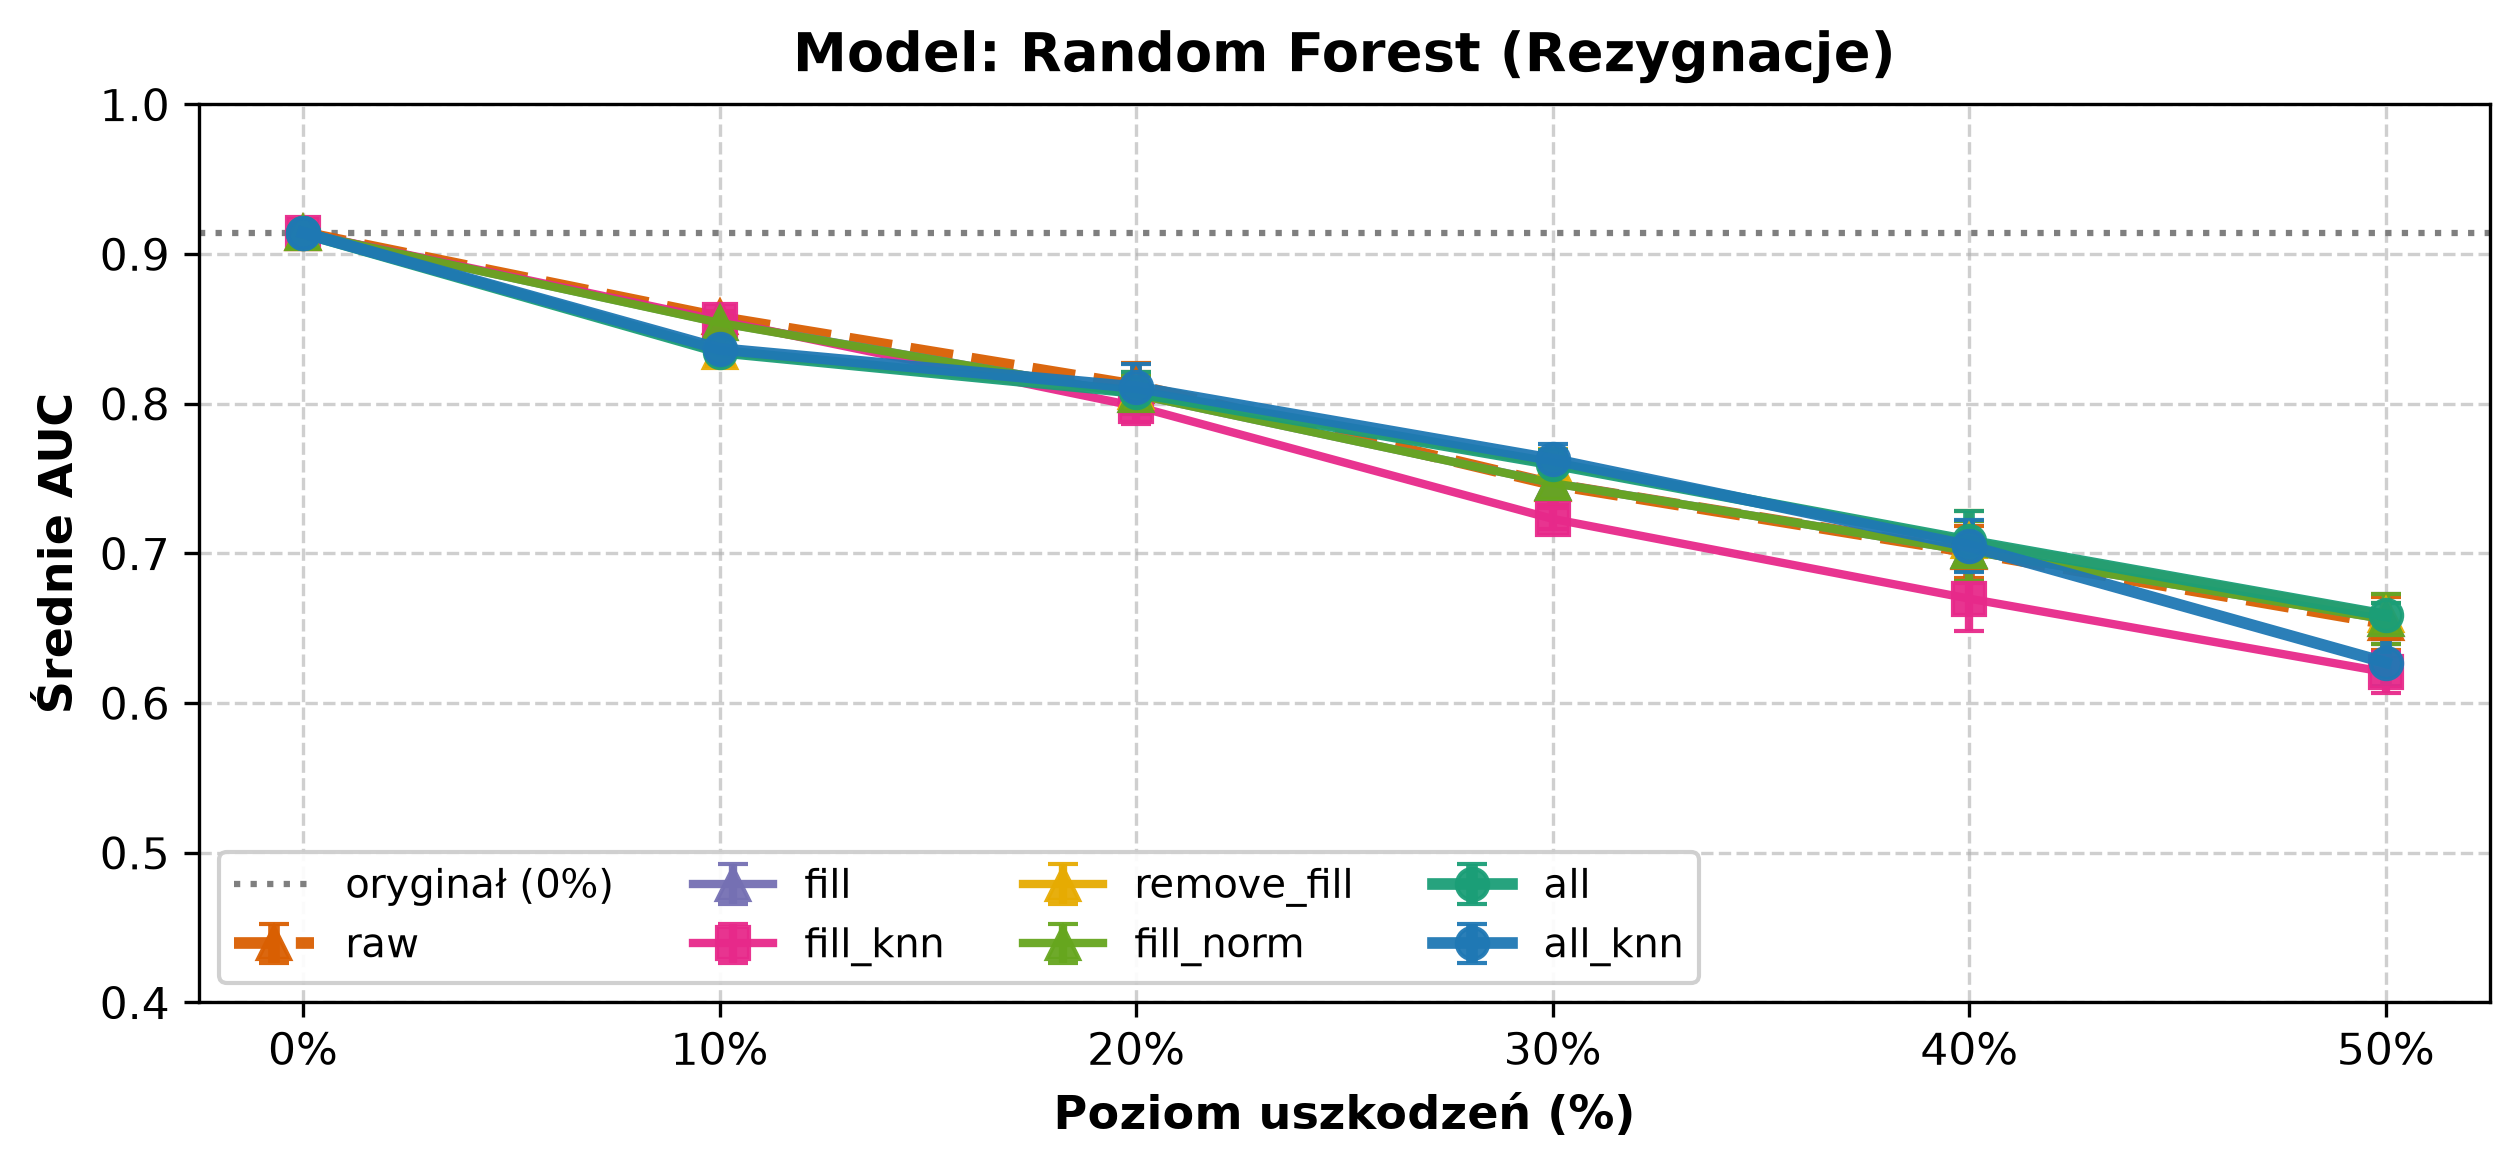
\includegraphics[width=\textwidth]{figures/Wykresy_Zaawansowane/1_Krzywe_Odpornosci/krzywa_rezygnacje_RF.png}
    \caption{Random Forest}
    \label{fig:odp_rezyg_rf}
\end{subfigure}
\vspace{0.25cm}
\begin{subfigure}[b]{0.92\textwidth}
    \centering
    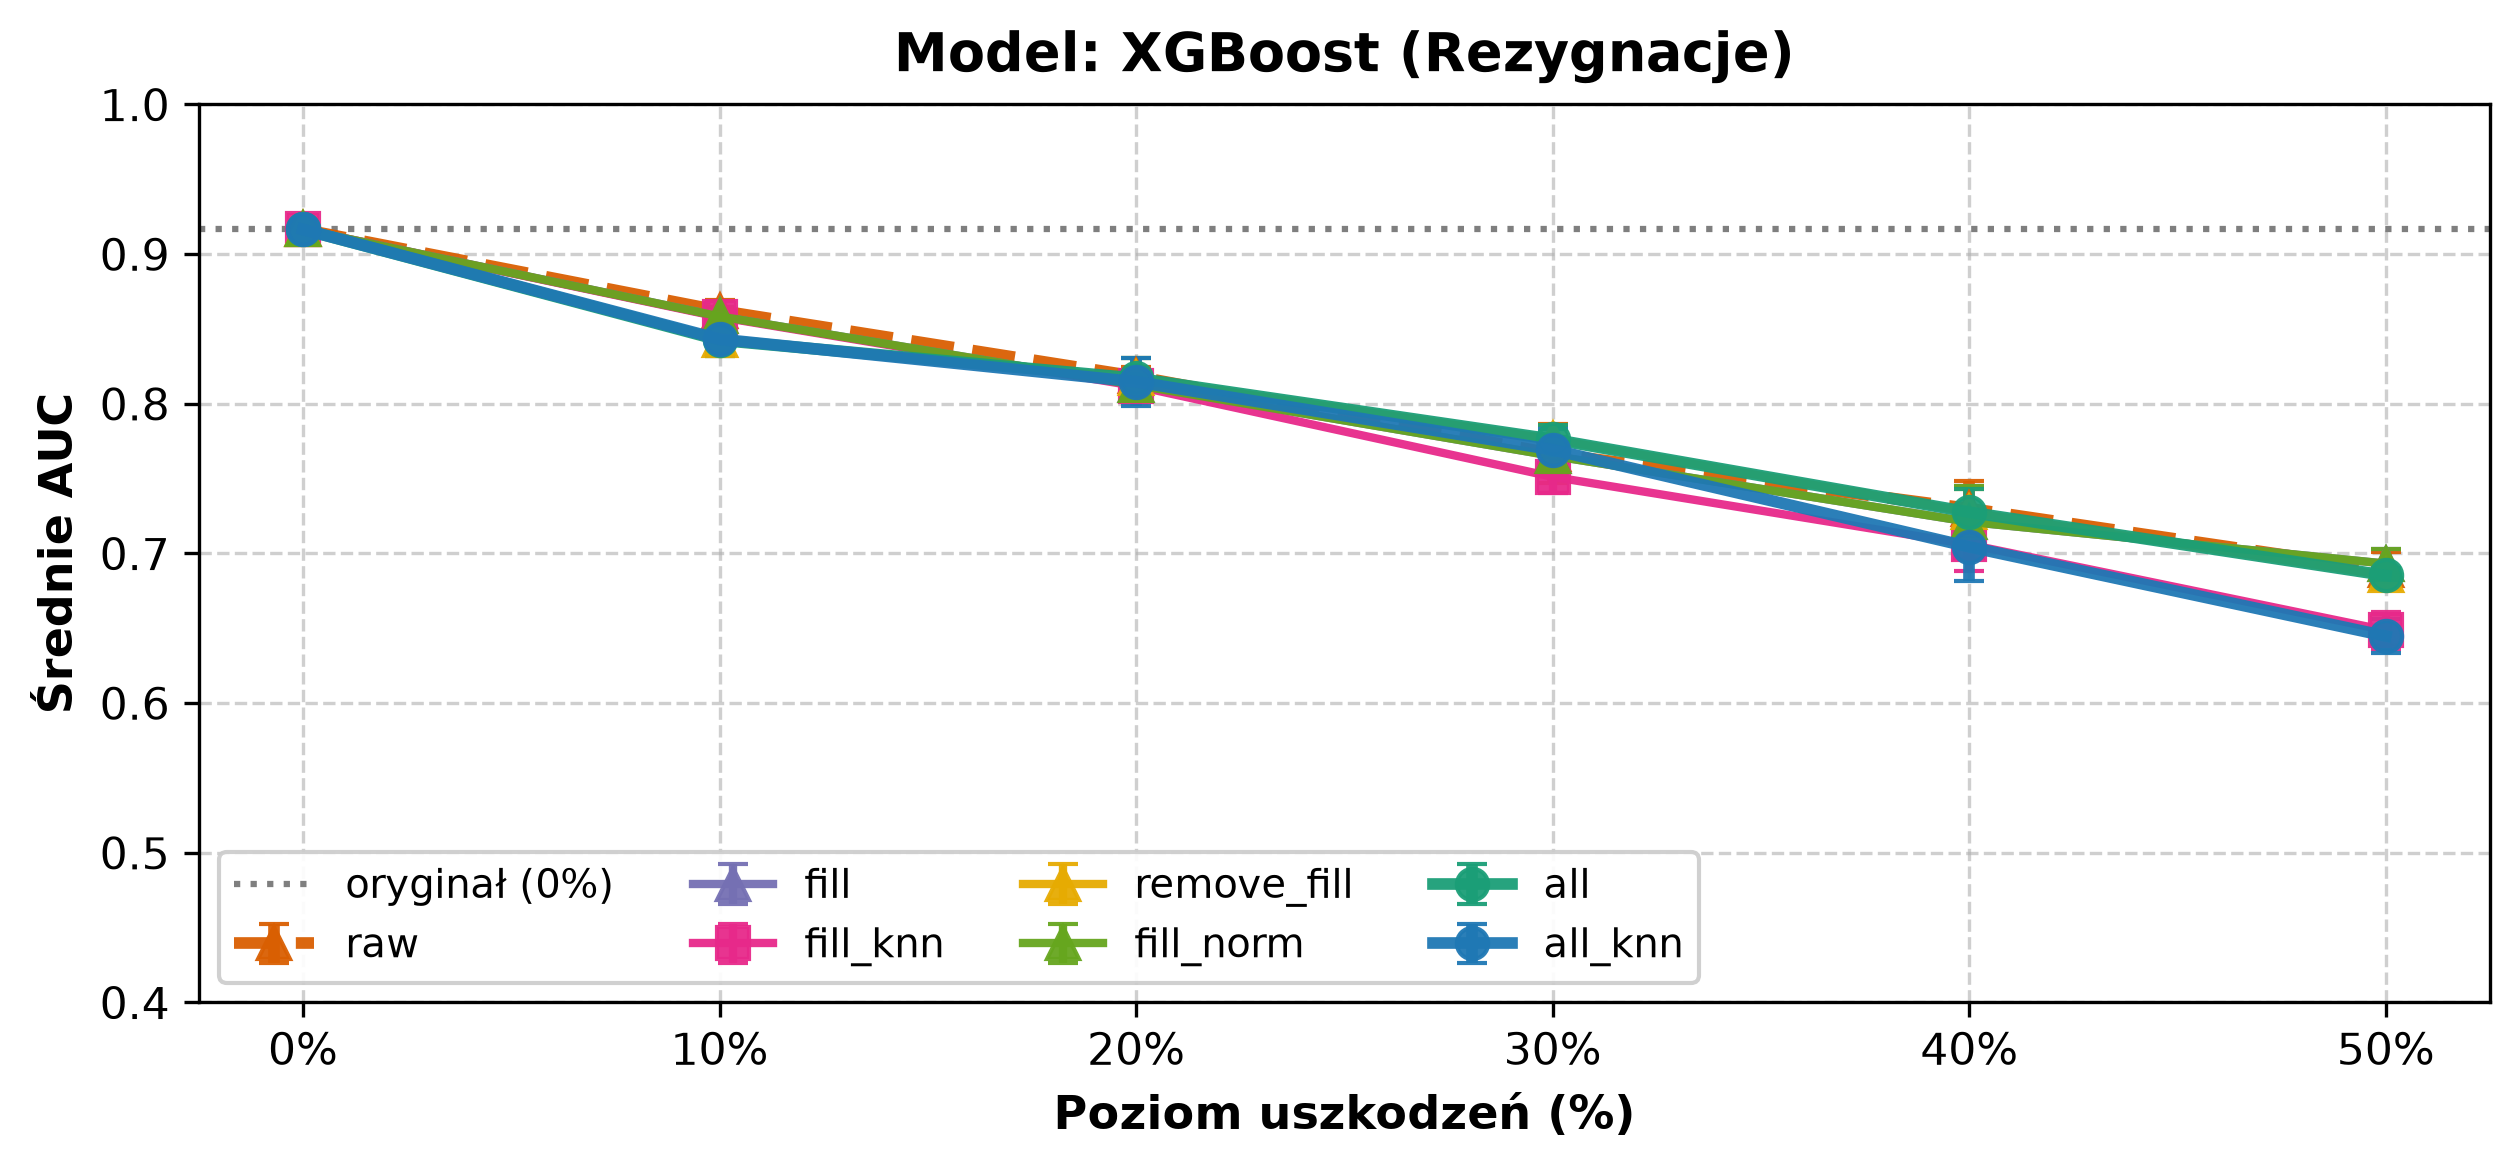
\includegraphics[width=\textwidth]{figures/Wykresy_Zaawansowane/1_Krzywe_Odpornosci/krzywa_rezygnacje_XGBoost.png}
    \caption{XGBoost}
    \label{fig:odp_rezyg_xgb}
\end{subfigure}
\caption{Krzywe odporności modeli zespołowych na zbiorze „Rezygnacje”}
\label{fig:odpornosc_rezygnacje_drzewa}
\end{figure}

\begin{figure}[H]
\centering
\begin{subfigure}[b]{0.92\textwidth}
    \centering
    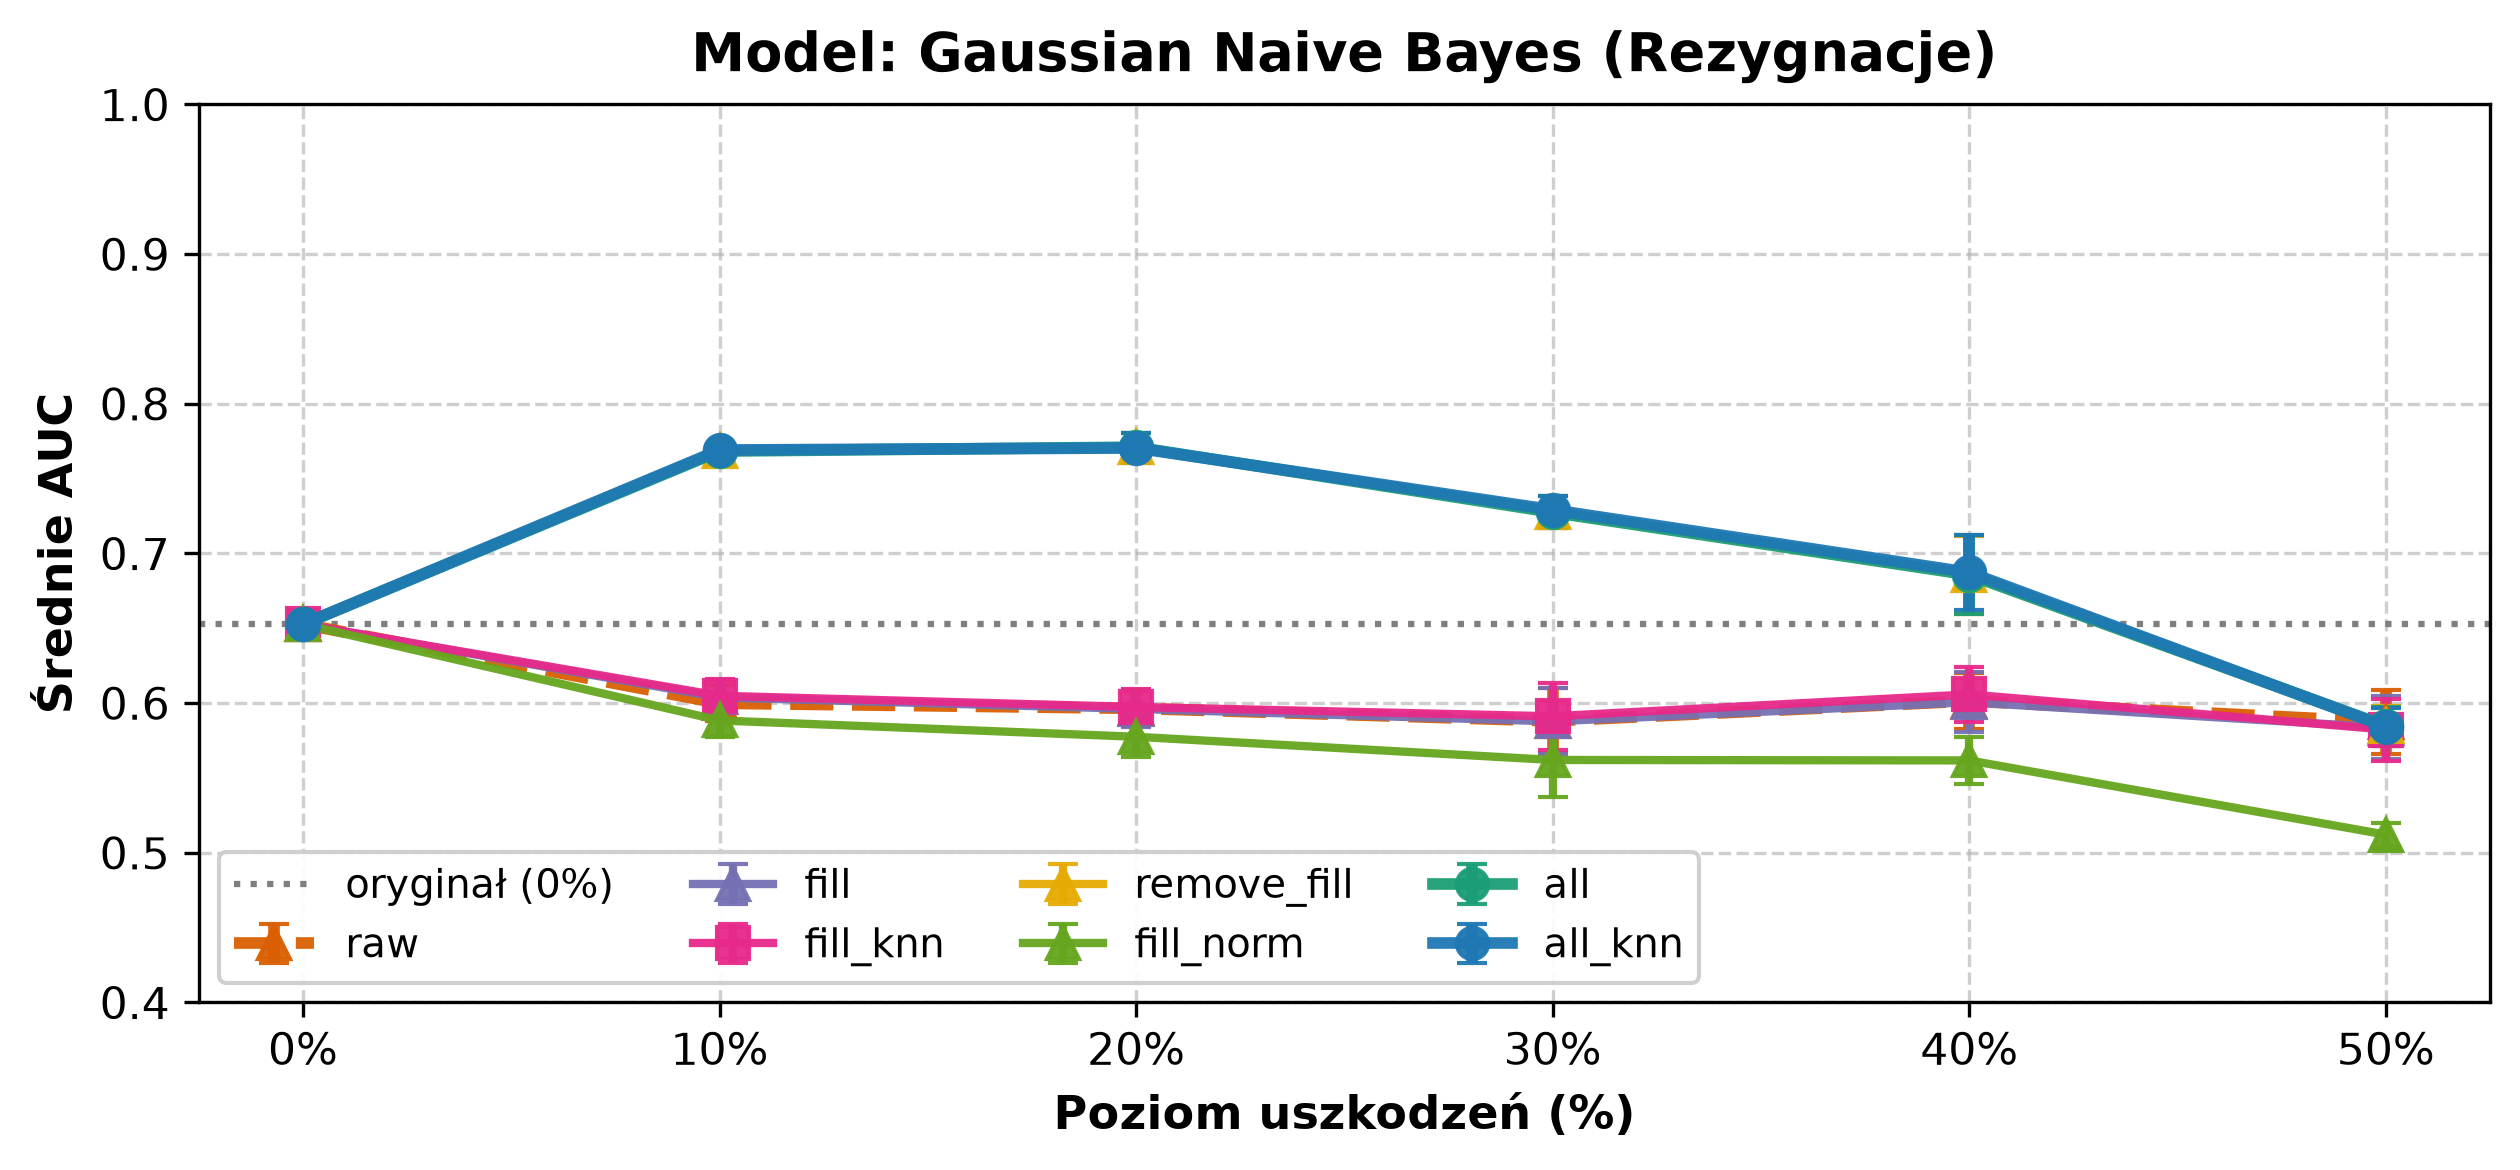
\includegraphics[width=\textwidth]{figures/Wykresy_Zaawansowane/1_Krzywe_Odpornosci/krzywa_rezygnacje_NB.png}
    \caption{Gaussian Naive Bayes}
    \label{fig:odp_rezyg_nb}
\end{subfigure}
\vspace{0.25cm}
\begin{subfigure}[b]{0.92\textwidth}
    \centering
    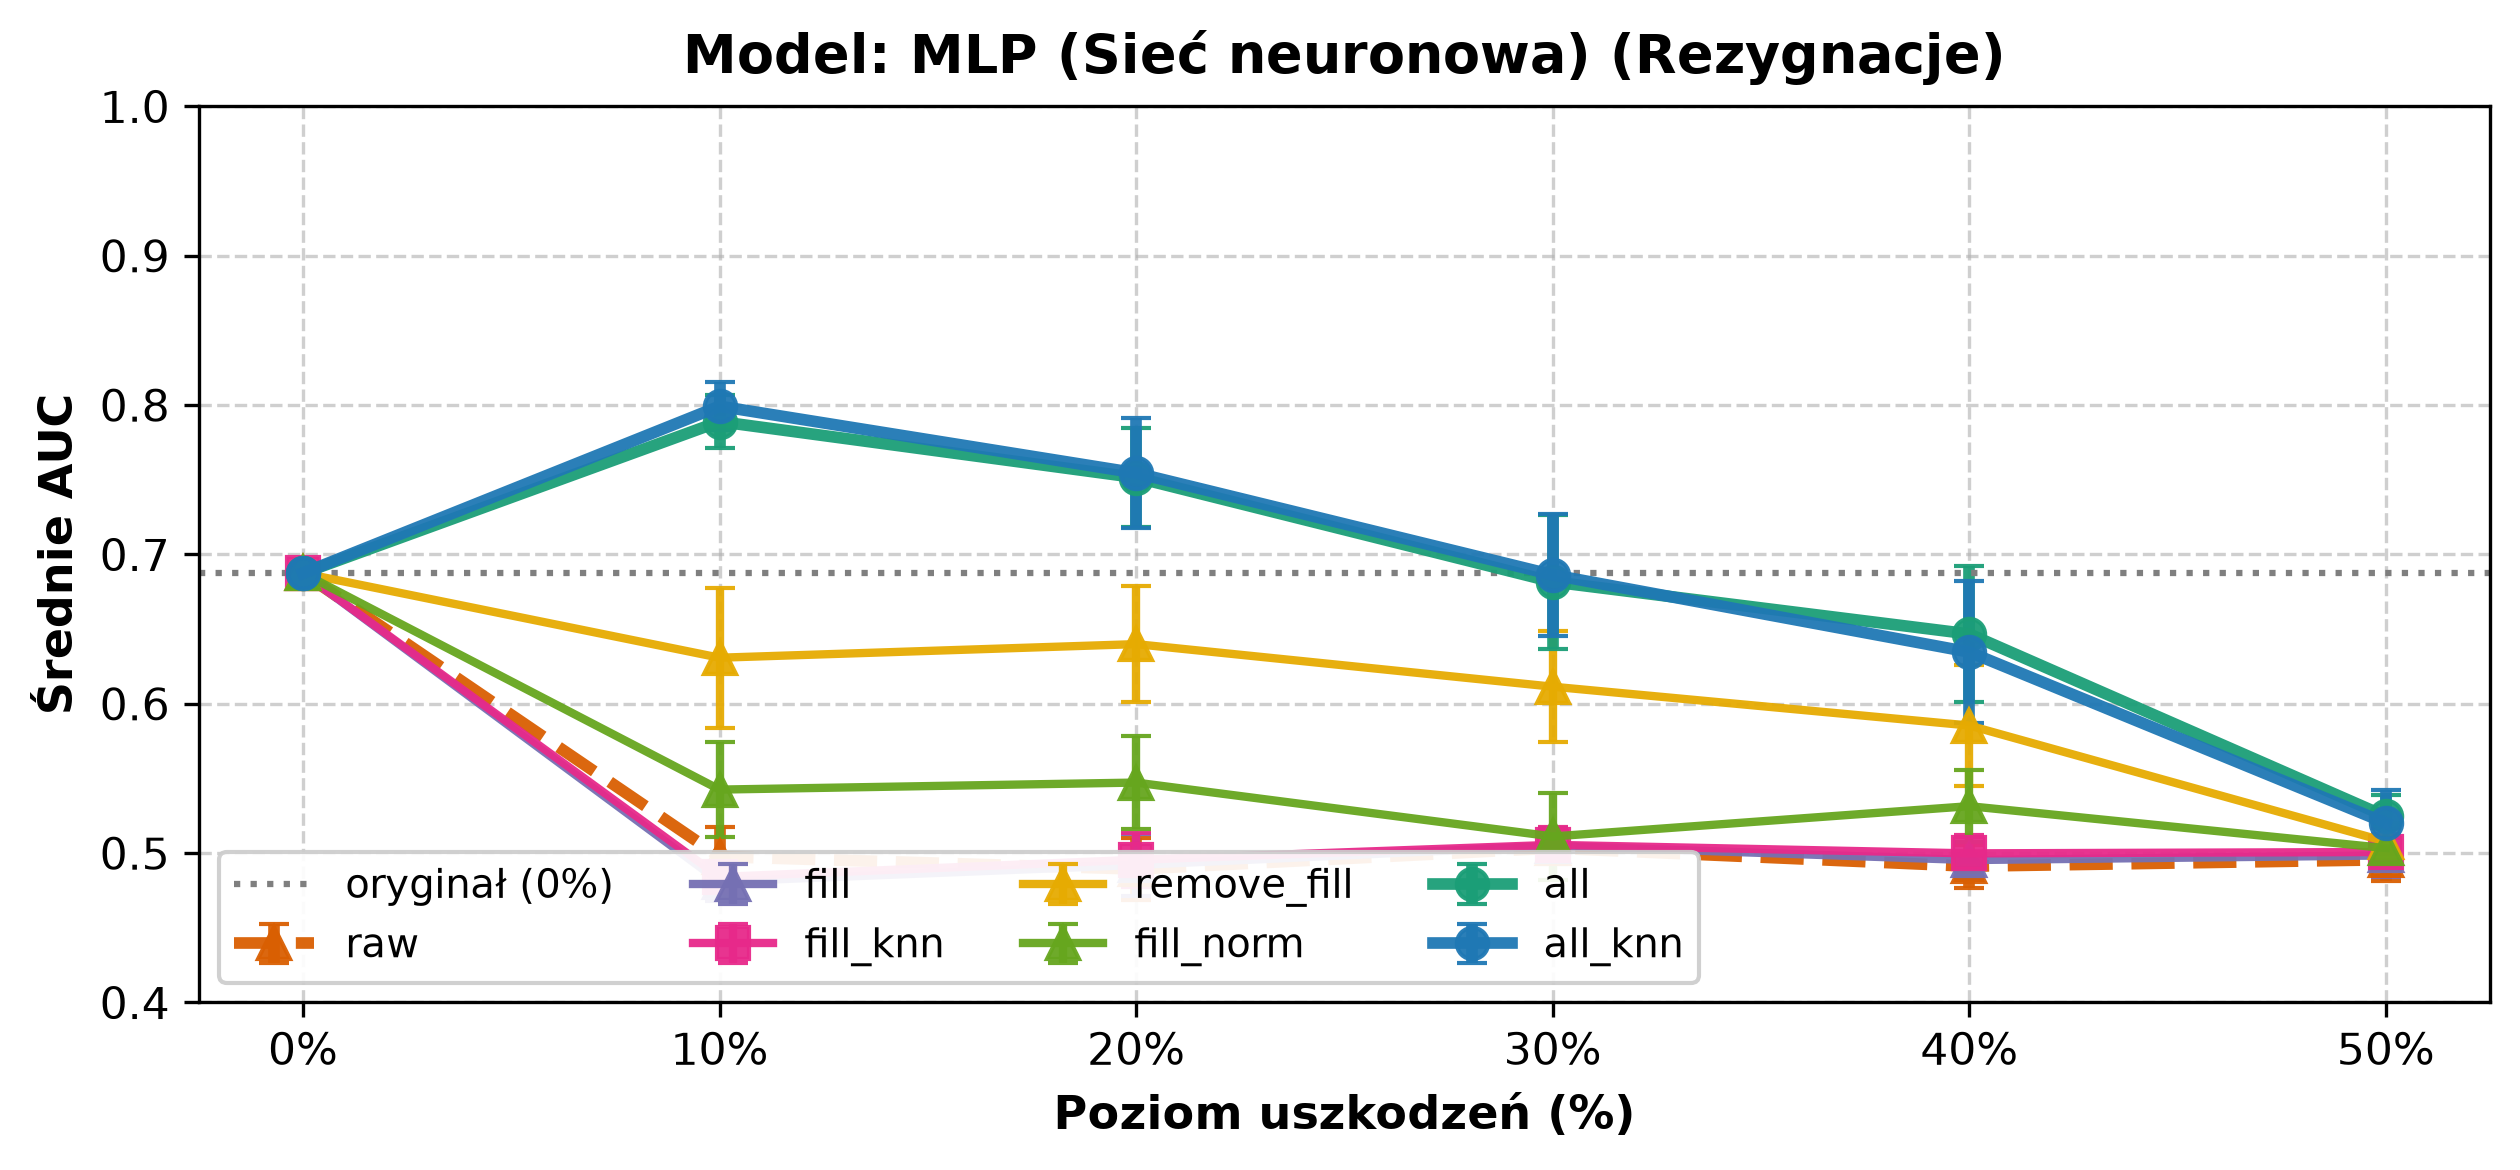
\includegraphics[width=\textwidth]{figures/Wykresy_Zaawansowane/1_Krzywe_Odpornosci/krzywa_rezygnacje_MLP.png}
    \caption{MLP (Sieć neuronowa)}
    \label{fig:odp_rezyg_mlp}
\end{subfigure}
\caption{Krzywe odporności klasyfikatora Bayesa i~sieci MLP na zbiorze „Rezygnacje”}
\label{fig:odpornosc_rezygnacje_inne}
\end{figure}

\begin{figure}[H]
\centering
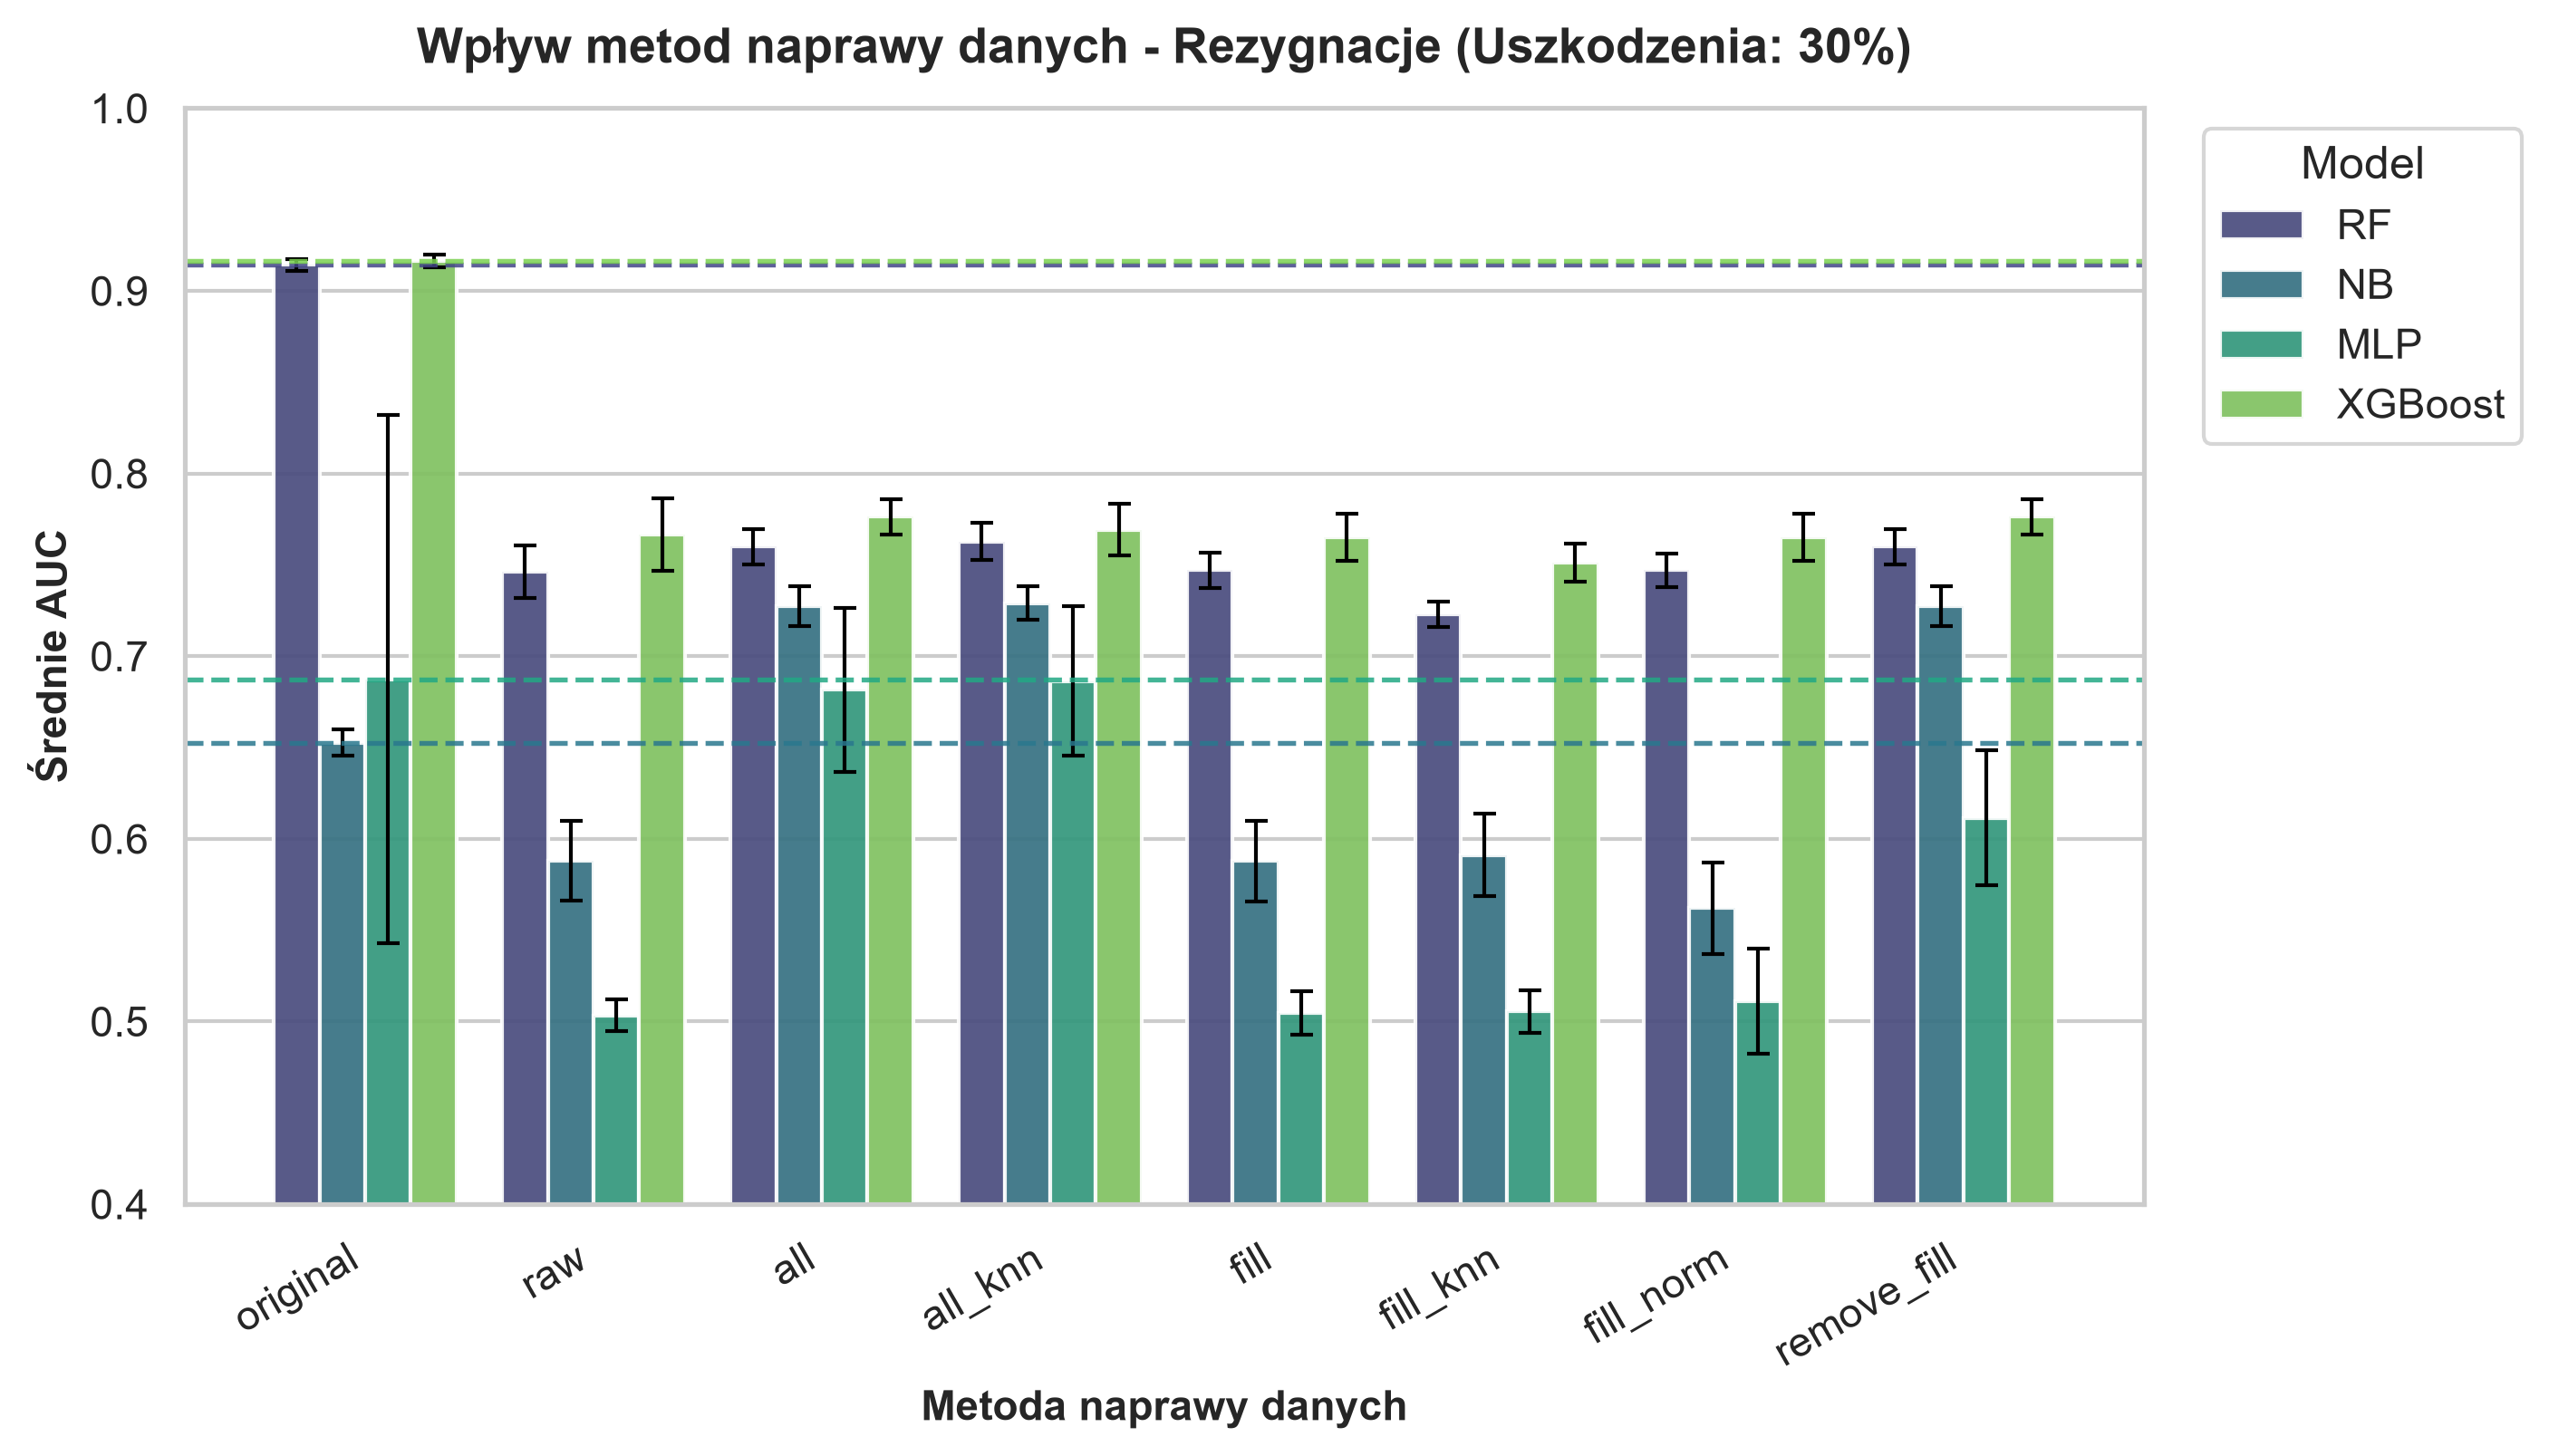
\includegraphics[width=0.95\textwidth]{figures/Wykresy_full/rezygnacje/rezygnacje_30proc.png}
\caption{Skuteczność strategii naprawy danych na zbiorze „Rezygnacje” przy uszkodzeniu 30\%}
\label{fig:slupkowy_rezygnacje_30}
\end{figure}

W~zbiorze telekomunikacyjnym (Tabela~\ref{tab:wyniki_rezygnacje}) modele zespołowe (XGBoost oraz Random Forest) wykazują najwyższą stabilność, osiągając $\mathrm{AUC} > 0{,}85$ przy $10\%$ uszkodzeń oraz zachowując $\mathrm{AUC} > 0{,}65 - 0{,}69$ nawet przy $50\%$ degradacji. Sieć MLP bez skalowania i~czyszczenia ulega załamaniu ($\mathrm{AUC} \approx 0{,}497$), jednak wdrożenie potoków \textit{all} oraz \textit{all\_knn} pozwala uzyskać zysk rzędu $+0{,}29$ AUC przy uszkodzeniu $10\%$ i~$+0{,}18$ AUC przy uszkodzeniu $30\%$.

\subsection{Ocena na zbiorze „Kredyty” (German Credit)}
Zbiór oceny ryzyka kredytowego zawiera liczne cechy kategoryczne i~jest zadaniem o~najniższej bazowej separowalności. Zestawienie wartości $\overline{\mathrm{AUC}}$ przedstawiono w~tabeli~\ref{tab:wyniki_kredyty}, natomiast wykresy odporności zilustrowano na rysunkach~\ref{fig:odpornosc_kredyty_drzewa}, \ref{fig:odpornosc_kredyty_inne} i~\ref{fig:slupkowy_kredyty_30}.

\begin{table}[H]
\centering
\caption{Wyniki $\overline{\mathrm{AUC}}$ na zbiorze „Kredyty” dla wszystkich poziomów degradacji}
\label{tab:wyniki_kredyty}
\vspace{0.2cm}
\resizebox{\textwidth}{!}{%
\begin{tabular}{llccccccc}
\toprule
\textbf{Model} & \textbf{Poziom} & \textbf{\texttt{raw}} & \textbf{\texttt{fill}} & \textbf{\texttt{fill\_knn}} & \textbf{\texttt{remove\_fill}} & \textbf{\texttt{fill\_norm}} & \textbf{\texttt{all}} & \textbf{\texttt{all\_knn}} \\
\midrule
\textbf{RF}      & 10\% & $\mathbf{0{,}6385}$ & $0{,}6322$ & $0{,}6291$ & $0{,}6350$ & $0{,}6320$ & $0{,}6347$ & $0{,}6335$ \\
                 & 20\% & $0{,}5992$ & $0{,}6003$ & $0{,}5880$ & $\mathbf{0{,}6014}$ & $0{,}6005$ & $0{,}6012$ & $0{,}5960$ \\
                 & 30\% & $0{,}5564$ & $0{,}5608$ & $0{,}5547$ & $\mathbf{0{,}5814}$ & $0{,}5610$ & $0{,}5812$ & $0{,}5813$ \\
                 & 40\% & $0{,}5275$ & $0{,}5401$ & $\mathbf{0{,}5471}$ & $0{,}5457$ & $0{,}5401$ & $0{,}5464$ & $0{,}5399$ \\
                 & 50\% & $0{,}5303$ & $0{,}5458$ & $\mathbf{0{,}5463}$ & $0{,}5402$ & $0{,}5456$ & $0{,}5401$ & $0{,}5394$ \\
\midrule
\textbf{XGBoost} & 10\% & $0{,}6462$ & $0{,}6443$ & $0{,}6384$ & $\mathbf{0{,}6516}$ & $0{,}6443$ & $\mathbf{0{,}6516}$ & $0{,}6455$ \\
                 & 20\% & $\mathbf{0{,}6127}$ & $0{,}6109$ & $0{,}6050$ & $0{,}6063$ & $0{,}6109$ & $0{,}6063$ & $0{,}6057$ \\
                 & 30\% & $0{,}5644$ & $0{,}5726$ & $0{,}5675$ & $\mathbf{0{,}5845}$ & $0{,}5726$ & $\mathbf{0{,}5845}$ & $0{,}5733$ \\
                 & 40\% & $0{,}5443$ & $0{,}5535$ & $0{,}5474$ & $\mathbf{0{,}5579}$ & $0{,}5535$ & $\mathbf{0{,}5579}$ & $0{,}5502$ \\
                 & 50\% & $0{,}5545$ & $0{,}5799$ & $0{,}5541$ & $\mathbf{0{,}5871}$ & $0{,}5799$ & $\mathbf{0{,}5871}$ & $0{,}5582$ \\
\midrule
\textbf{NB}      & 10\% & $0{,}5613$ & $0{,}5575$ & $0{,}5463$ & $\mathbf{0{,}6112}$ & $0{,}5743$ & $0{,}6059$ & $0{,}6068$ \\
                 & 20\% & $0{,}5417$ & $0{,}5436$ & $0{,}5276$ & $\mathbf{0{,}6056}$ & $0{,}5716$ & $0{,}6022$ & $0{,}5973$ \\
                 & 30\% & $0{,}5076$ & $0{,}5035$ & $0{,}5105$ & $0{,}5703$ & $0{,}5654$ & $0{,}5691$ & $\mathbf{0{,}5713}$ \\
                 & 40\% & $0{,}4917$ & $0{,}4983$ & $0{,}5121$ & $0{,}5442$ & $0{,}5454$ & $0{,}5512$ & $\mathbf{0{,}5530}$ \\
                 & 50\% & $0{,}5144$ & $0{,}5263$ & $0{,}5209$ & $0{,}5477$ & $\mathbf{0{,}5682}$ & $0{,}5611$ & $0{,}5621$ \\
\midrule
\textbf{MLP}     & 10\% & $0{,}4589$ & $0{,}4668$ & $0{,}4662$ & $0{,}5062$ & $0{,}4909$ & $\mathbf{0{,}6055}$ & $0{,}5907$ \\
                 & 20\% & $0{,}4795$ & $0{,}4742$ & $0{,}4771$ & $0{,}4854$ & $0{,}5002$ & $\mathbf{0{,}5786}$ & $0{,}5681$ \\
                 & 30\% & $0{,}4740$ & $0{,}4854$ & $0{,}4880$ & $0{,}5075$ & $0{,}5052$ & $0{,}5506$ & $\mathbf{0{,}5538}$ \\
                 & 40\% & $0{,}4866$ & $0{,}4793$ & $0{,}4847$ & $0{,}4772$ & $0{,}4822$ & $0{,}5162$ & $\mathbf{0{,}5217}$ \\
                 & 50\% & $0{,}4935$ & $0{,}4803$ & $0{,}4704$ & $0{,}4871$ & $\mathbf{0{,}5097}$ & $0{,}5074$ & $0{,}4957$ \\
\bottomrule
\end{tabular}%
}
\end{table}

\begin{figure}[H]
\centering
\begin{subfigure}[b]{0.92\textwidth}
    \centering
    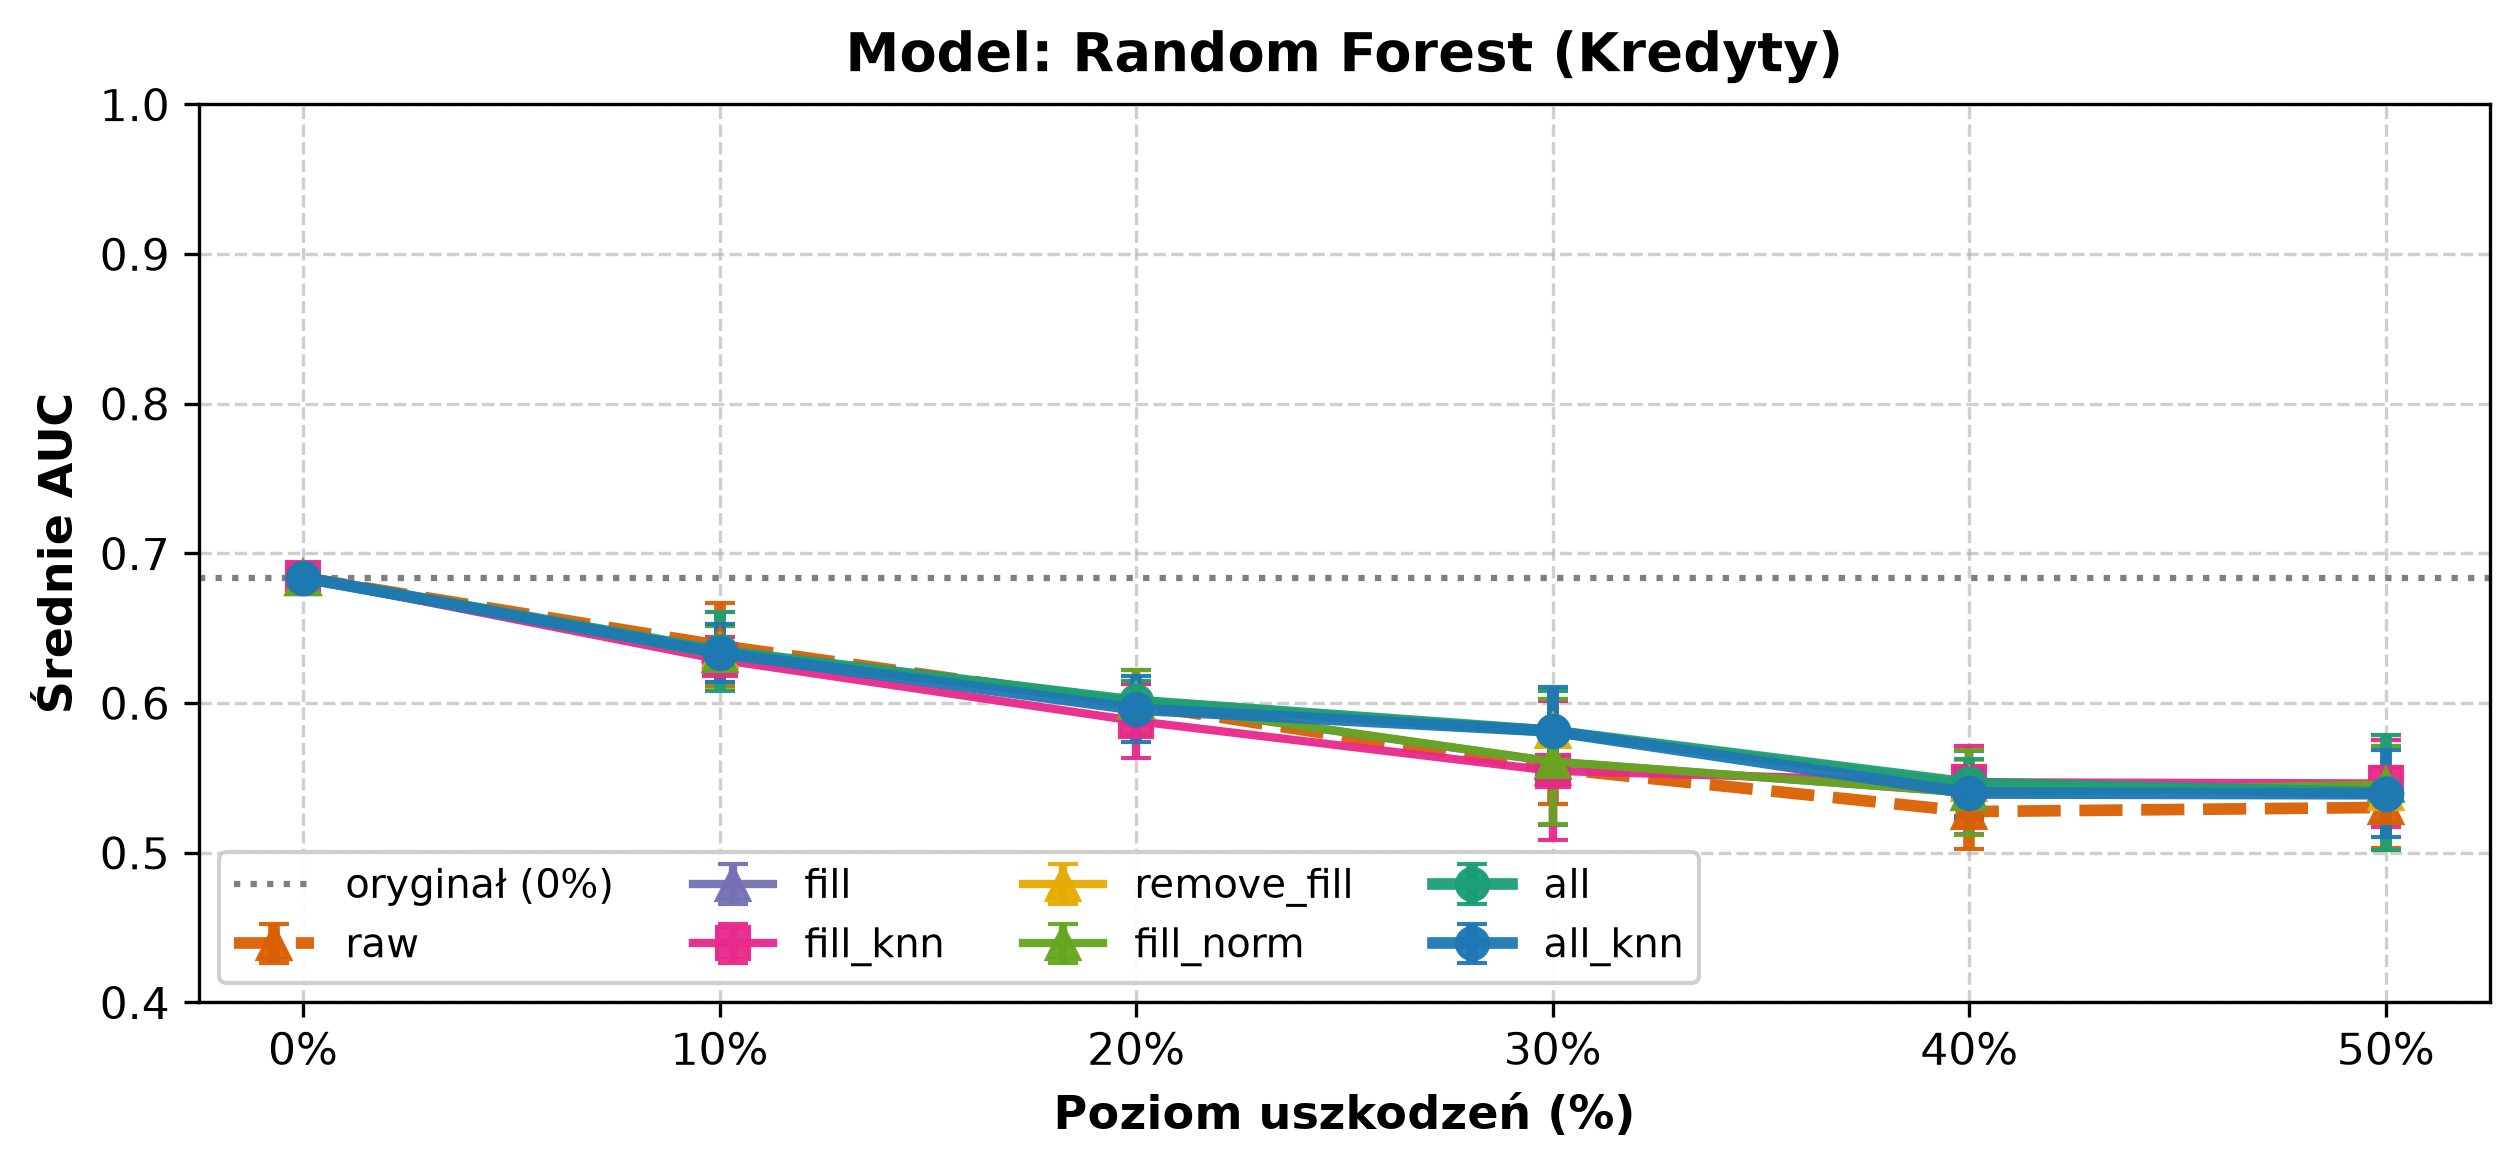
\includegraphics[width=\textwidth]{figures/Wykresy_Zaawansowane/1_Krzywe_Odpornosci/krzywa_kredyty_RF.png}
    \caption{Random Forest}
    \label{fig:odp_kred_rf}
\end{subfigure}
\vspace{0.25cm}
\begin{subfigure}[b]{0.92\textwidth}
    \centering
    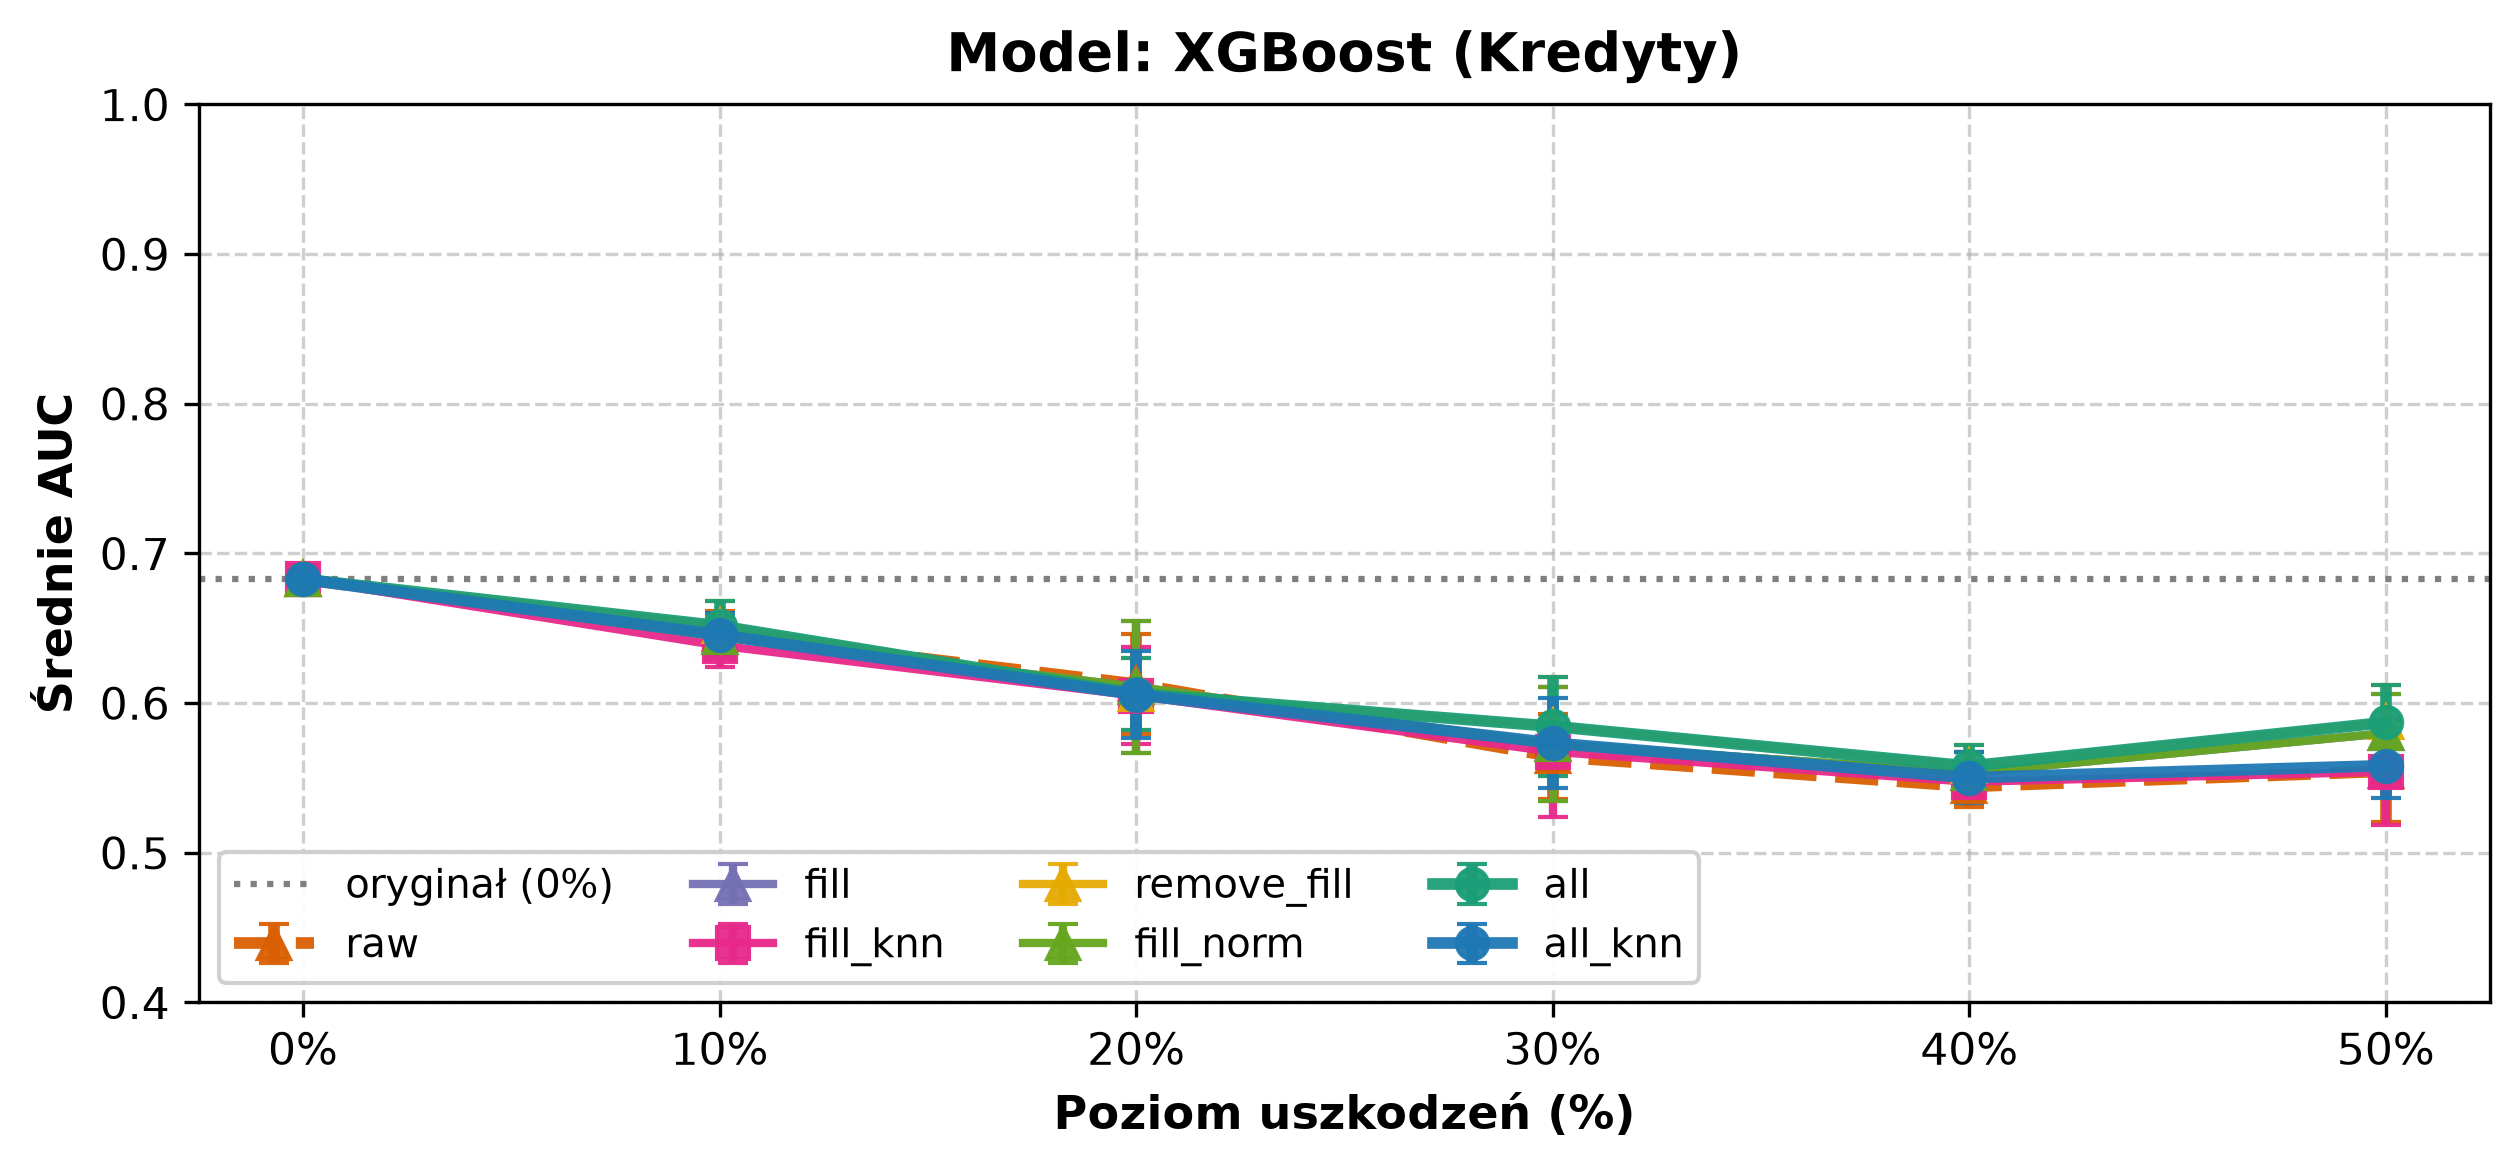
\includegraphics[width=\textwidth]{figures/Wykresy_Zaawansowane/1_Krzywe_Odpornosci/krzywa_kredyty_XGBoost.png}
    \caption{XGBoost}
    \label{fig:odp_kred_xgb}
\end{subfigure}
\caption{Krzywe odporności modeli zespołowych na zbiorze „Kredyty”}
\label{fig:odpornosc_kredyty_drzewa}
\end{figure}

\begin{figure}[H]
\centering
\begin{subfigure}[b]{0.92\textwidth}
    \centering
    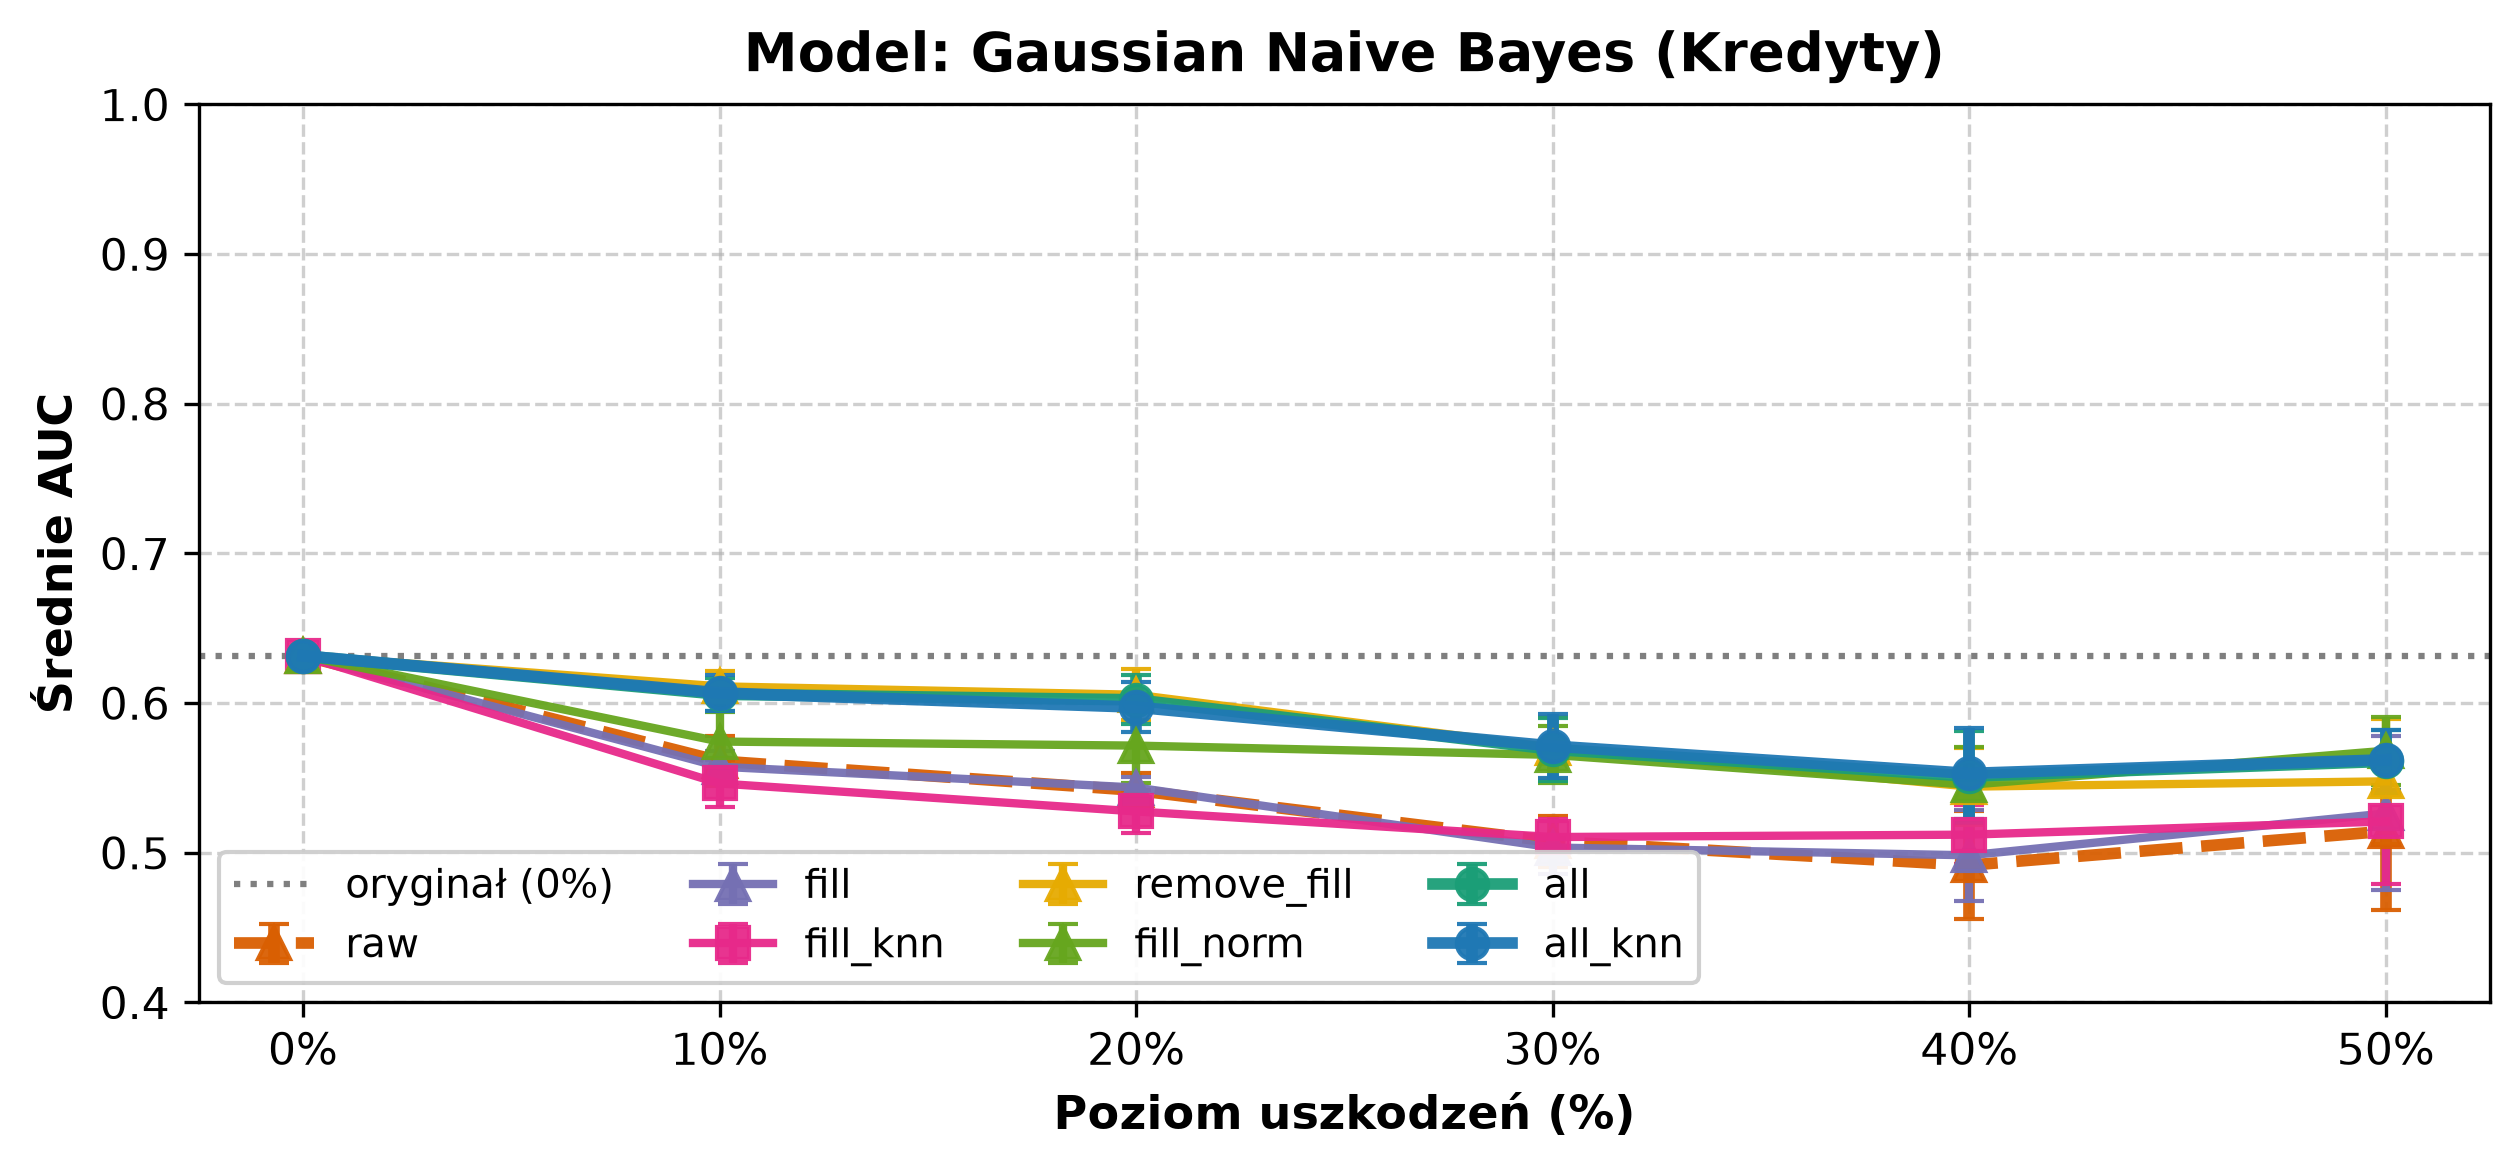
\includegraphics[width=\textwidth]{figures/Wykresy_Zaawansowane/1_Krzywe_Odpornosci/krzywa_kredyty_NB.png}
    \caption{Gaussian Naive Bayes}
    \label{fig:odp_kred_nb}
\end{subfigure}
\vspace{0.25cm}
\begin{subfigure}[b]{0.92\textwidth}
    \centering
    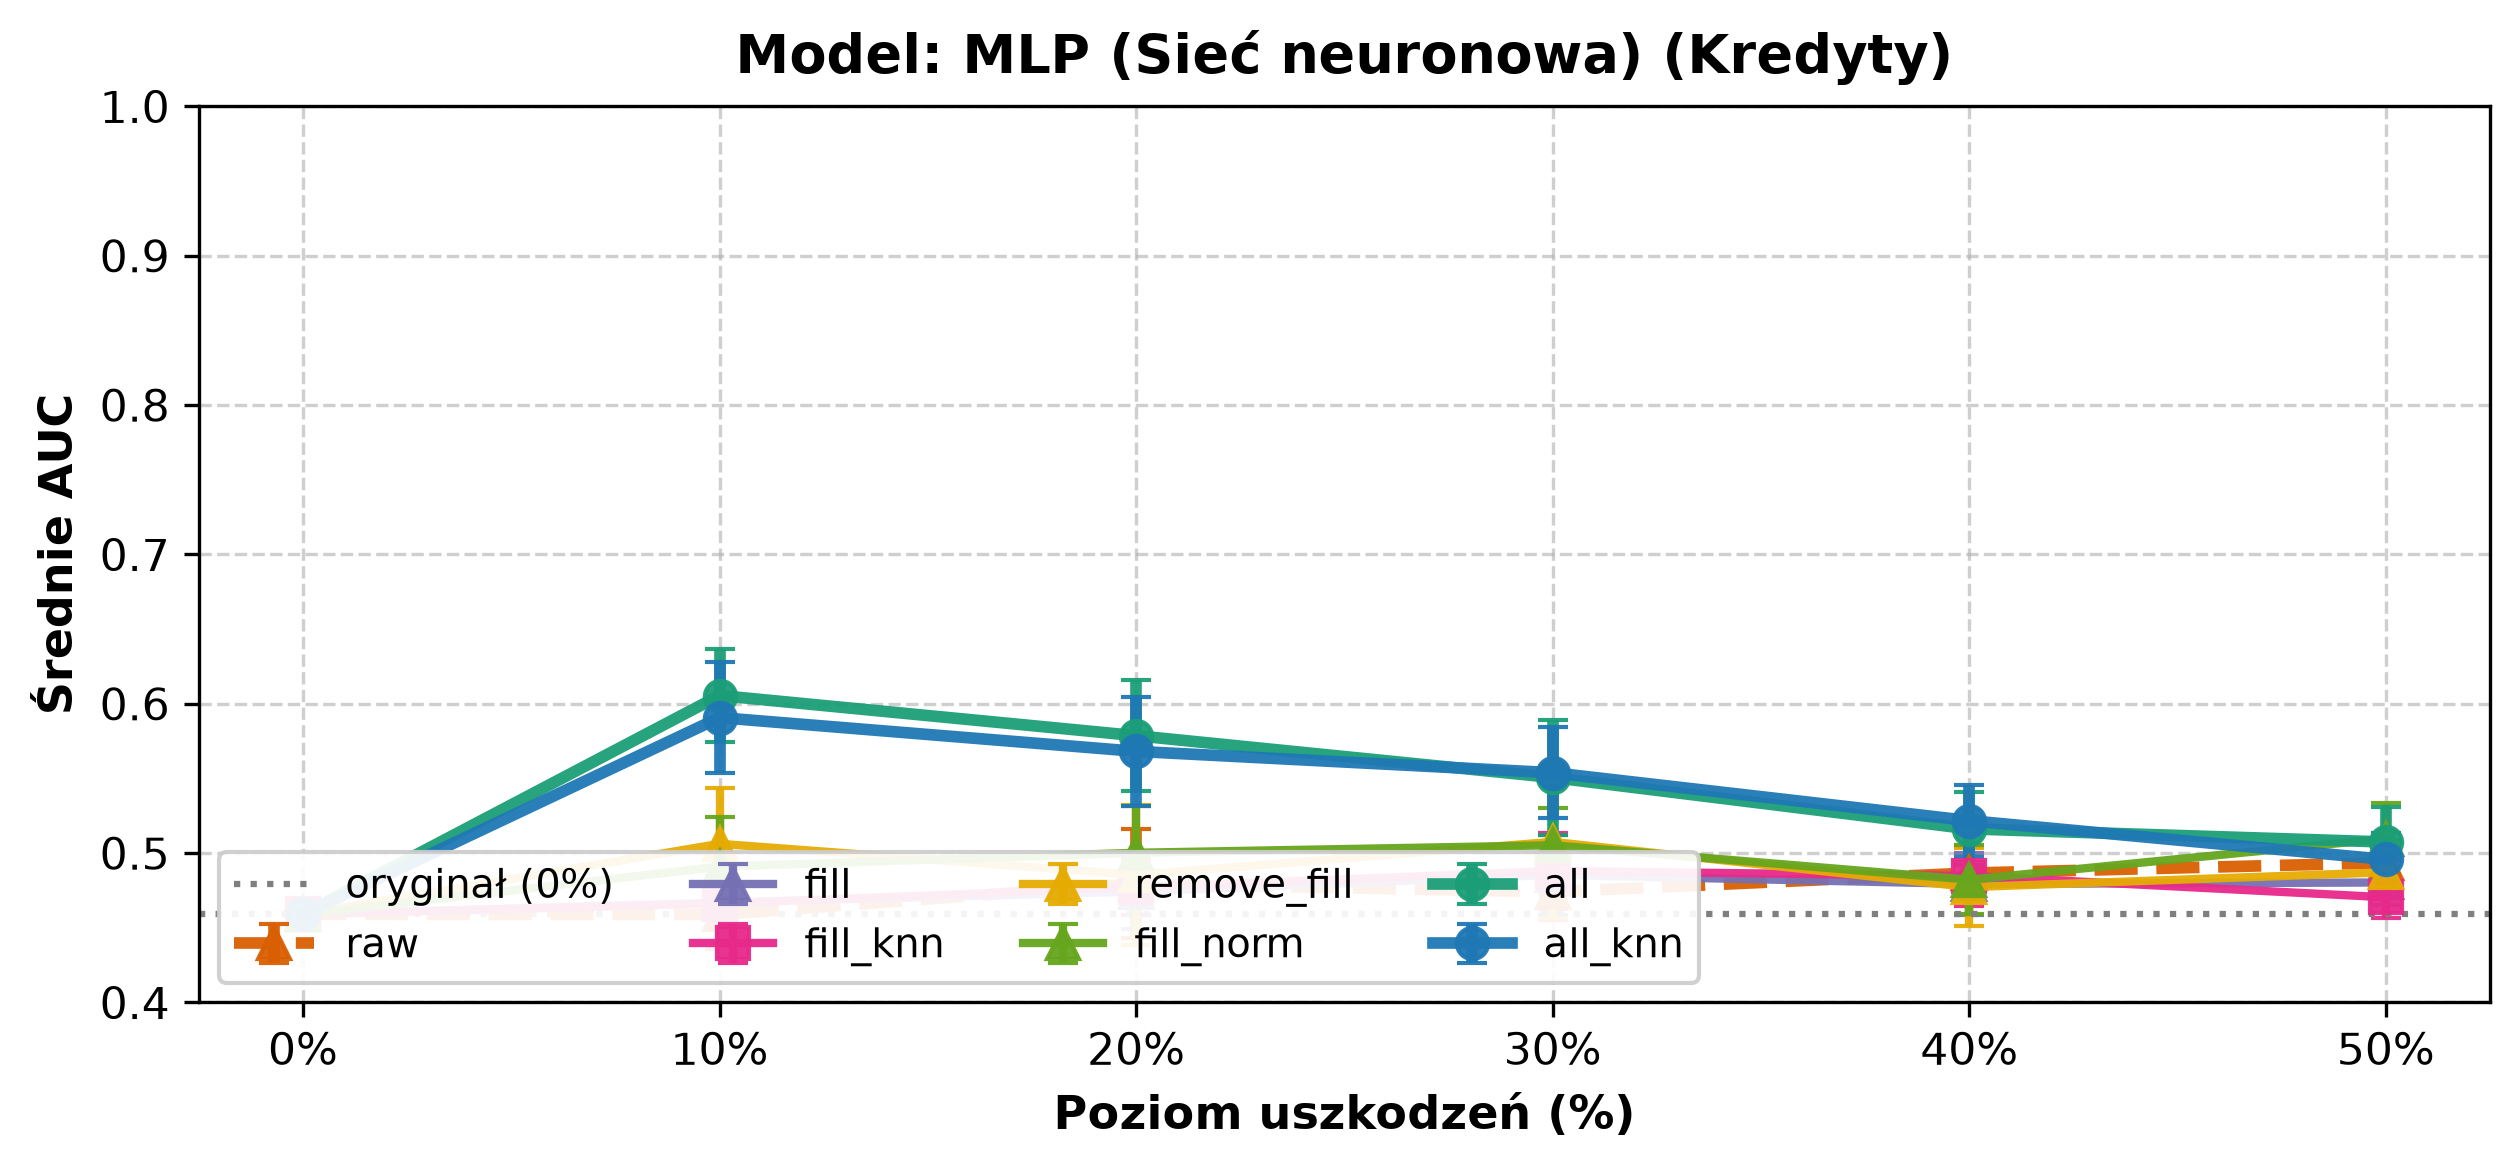
\includegraphics[width=\textwidth]{figures/Wykresy_Zaawansowane/1_Krzywe_Odpornosci/krzywa_kredyty_MLP.png}
    \caption{MLP (Sieć neuronowa)}
    \label{fig:odp_kred_mlp}
\end{subfigure}
\caption{Krzywe odporności klasyfikatora Bayesa i~sieci MLP na zbiorze „Kredyty”}
\label{fig:odpornosc_kredyty_inne}
\end{figure}

\begin{figure}[H]
\centering
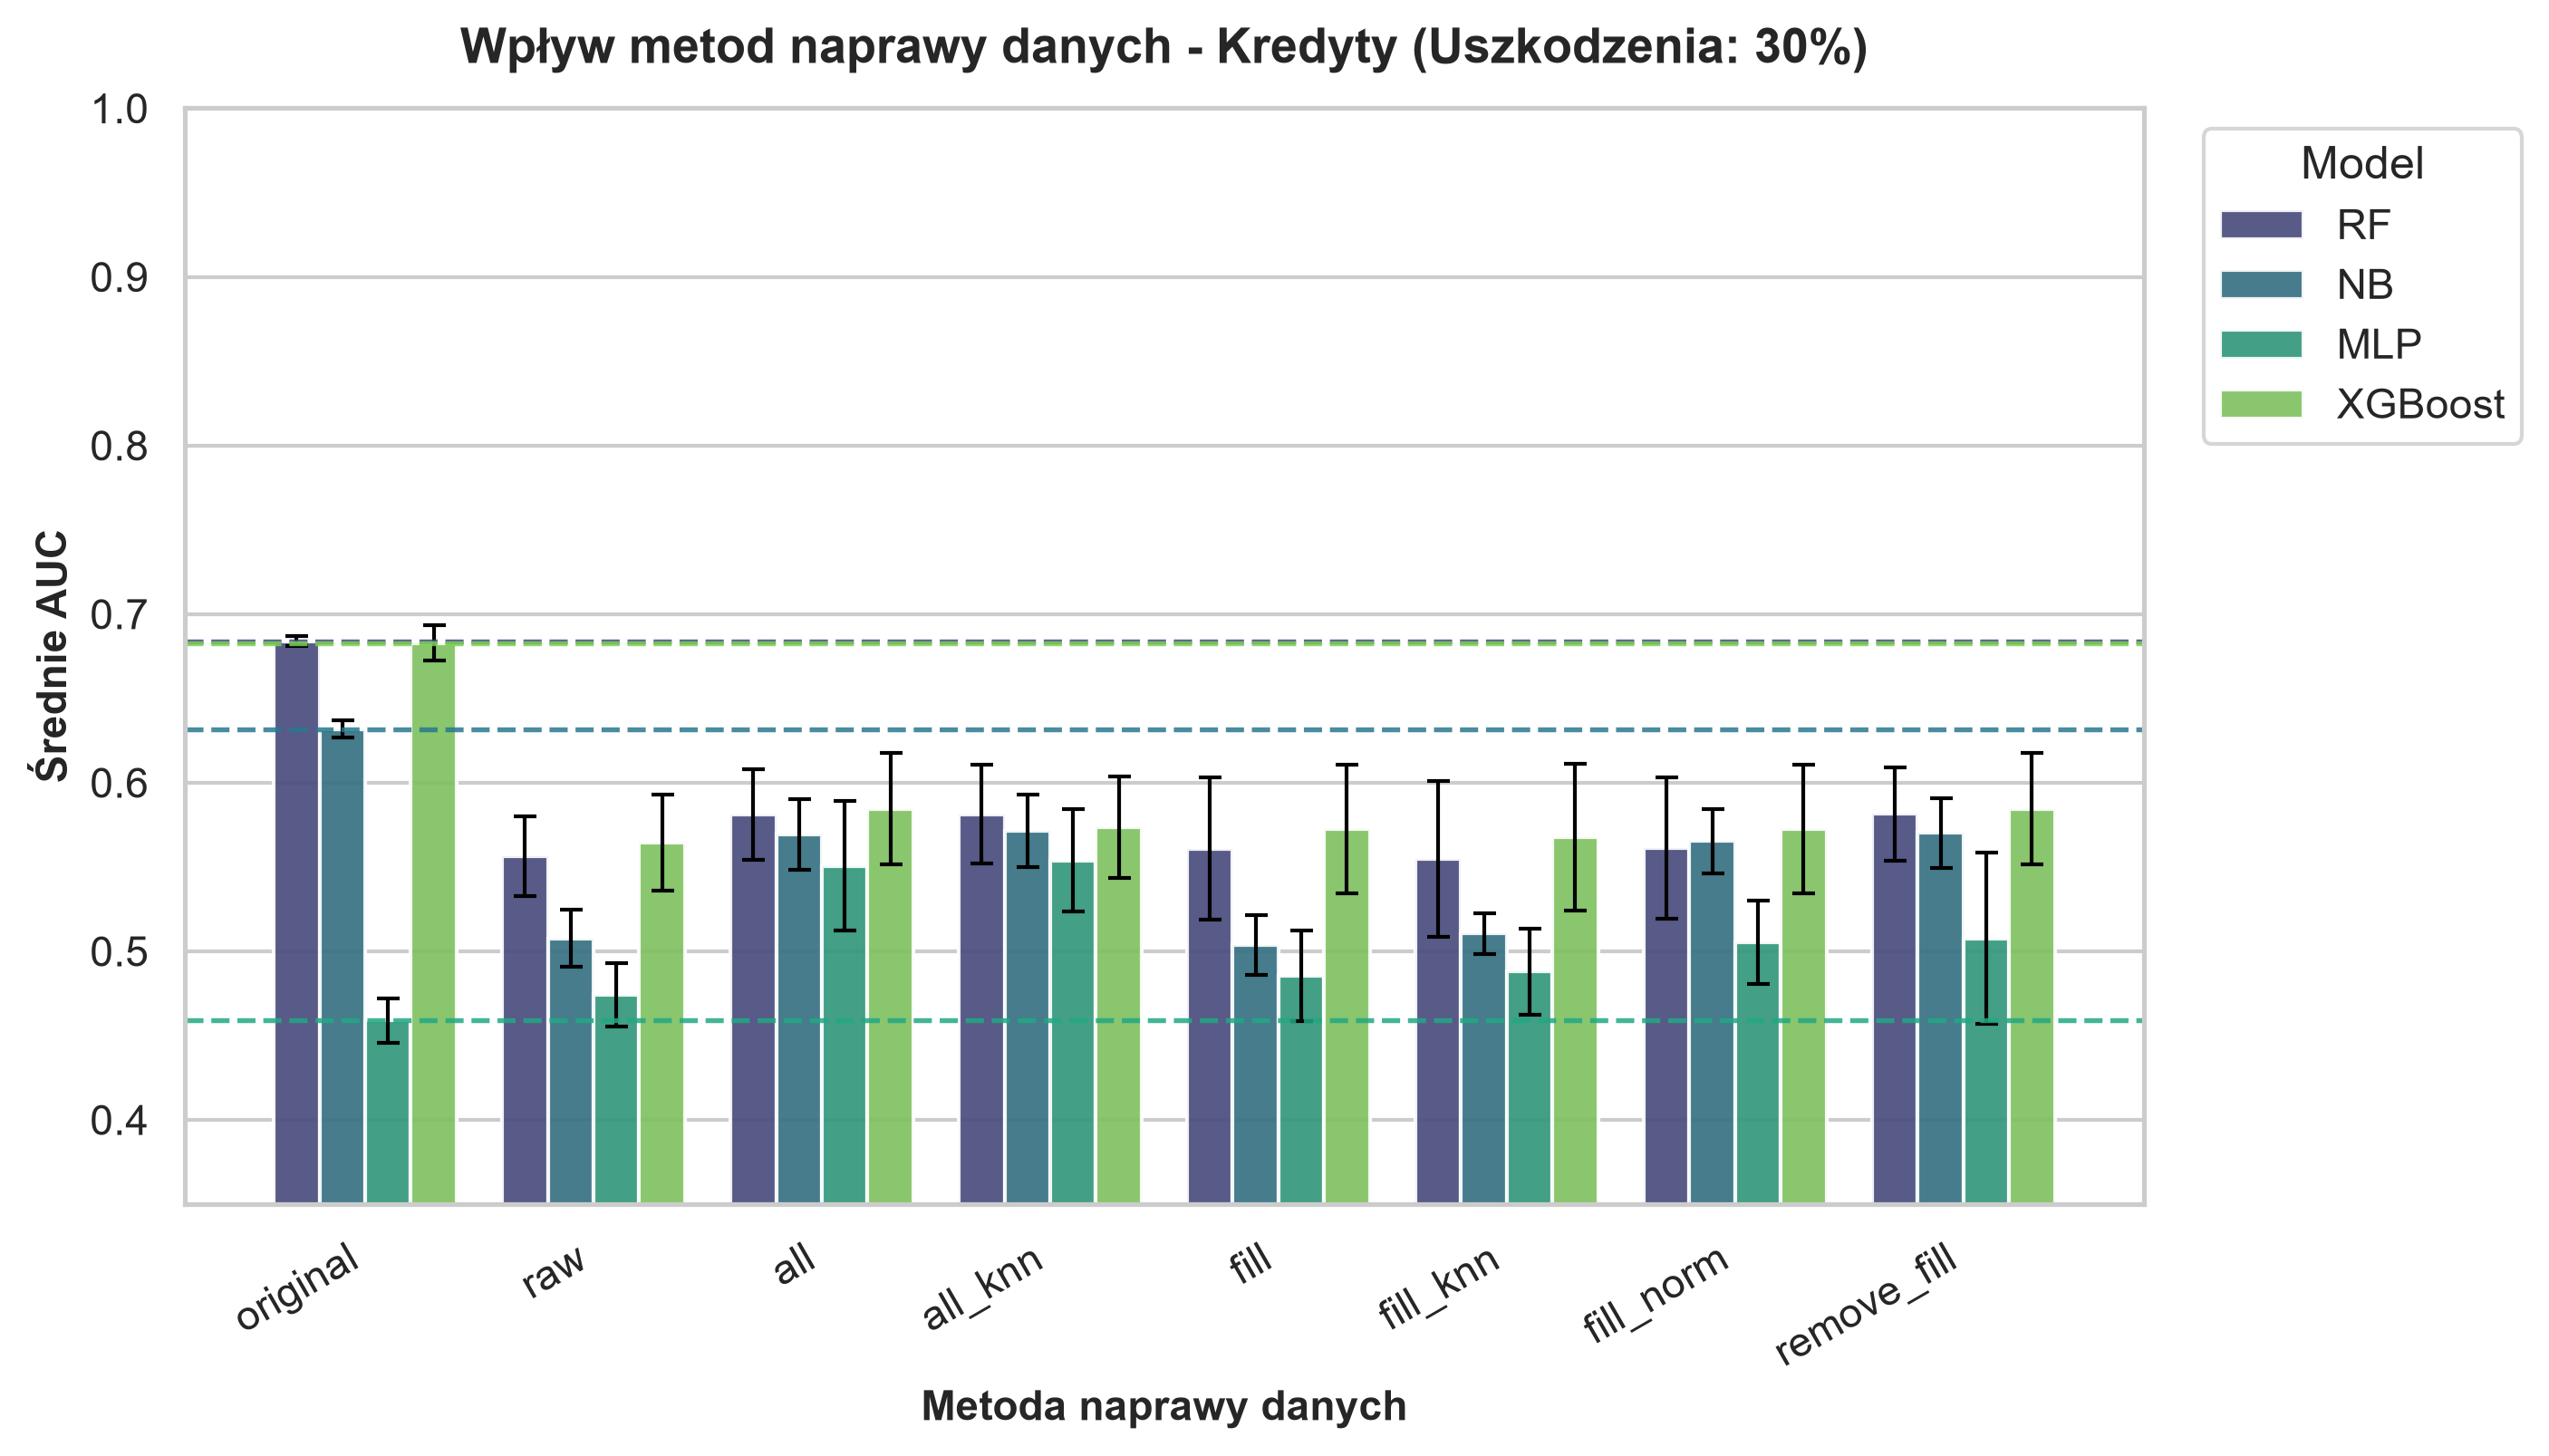
\includegraphics[width=0.95\textwidth]{figures/Wykresy_full/kredyty/kredyty_30proc.png}
\caption{Porównanie modeli i~metod czyszczenia na zbiorze „Kredyty” przy poziomie uszkodzeń 30\%}
\label{fig:slupkowy_kredyty_30}
\end{figure}

\section{Analiza zysku z~czyszczenia danych ($\Delta \mathrm{AUC}$)}
Aby dokonać całościowej syntezy zysków z~poszczególnych strategii czyszczenia danych, wygenerowano zestawienie średniego zysku $\Delta \mathrm{AUC}$ w~przekroju modeli oraz badanych zbiorów danych (Tabela~\ref{tab:delta_auc_summary}). Następnie przeanalizowano rozkłady zysków za pomocą dedykowanych heatmap w~trzech kluczowych płaszczyznach badawczych.

\begin{table}[H]
\centering
\caption{Średni zysk predykcyjny ($\Delta \mathrm{AUC}$) w~stosunku do danych surowych (\texttt{raw}) w~przekroju modeli i~zbiorów danych}
\label{tab:delta_auc_summary}
\vspace{0.2cm}
\resizebox{\textwidth}{!}{%
\begin{tabular}{lcccccc}
\toprule
\textbf{Przekrój badawczy} & \textbf{\texttt{fill}} & \textbf{\texttt{fill\_knn}} & \textbf{\texttt{remove\_fill}} & \textbf{\texttt{fill\_norm}} & \textbf{\texttt{all}} & \textbf{\texttt{all\_knn}} \\
\midrule
\textbf{MLP (Sieć neuronowa)} & $+0{,}0022$ & $-0{,}0020$ & $+0{,}0327$ & $+0{,}0999$ & $\mathbf{+0{,}1758}$ & $+0{,}1717$ \\
\textbf{Gaussian NB}          & $-0{,}0035$ & $-0{,}0048$ & $+0{,}0905$ & $-0{,}0128$ & $+0{,}1033$ & $\mathbf{+0{,}1059}$ \\
\textbf{Random Forest}        & $+0{,}0006$ & $-0{,}0069$ & $-0{,}0030$ & $+0{,}0006$ & $-0{,}0031$ & $-0{,}0073$ \\
\textbf{XGBoost}              & $+0{,}0016$ & $-0{,}0084$ & $+0{,}0002$ & $+0{,}0016$ & $+0{,}0002$ & $-0{,}0112$ \\
\midrule
\textit{Zbiór: Zapalenia naczyń} & $+0{,}0020$ & $-0{,}0071$ & $+0{,}0186$ & $+0{,}0523$ & $\mathbf{+0{,}0906}$ & $+0{,}0905$ \\
\textit{Zbiór: Serce}            & $-0{,}0054$ & $-0{,}0103$ & $-0{,}0050$ & $+0{,}0372$ & $\mathbf{+0{,}0484}$ & $+0{,}0482$ \\
\textit{Zbiór: Diabetes}         & $+0{,}0023$ & $-0{,}0014$ & $+0{,}0622$ & $+0{,}0054$ & $\mathbf{+0{,}0953}$ & $+0{,}0837$ \\
\textit{Zbiór: Rezygnacje}       & $-0{,}0014$ & $-0{,}0088$ & $+0{,}0522$ & $-0{,}0017$ & $\mathbf{+0{,}0731}$ & $+0{,}0684$ \\
\textit{Zbiór: Kredyty}          & $+0{,}0036$ & $-0{,}0001$ & $+0{,}0225$ & $+0{,}0185$ & $\mathbf{+0{,}0378}$ & $+0{,}0330$ \\
\bottomrule
\end{tabular}%
}
\end{table}

Rysunek~\ref{fig:heatmapa_model} przedstawia zależność zysku od rodziny klasyfikatora, rysunek~\ref{fig:heatmapa_dataset} w~przekroju zbiorów danych, a~rysunek~\ref{fig:heatmapa_poziom} w~funkcji nasilenia zanieczyszczeń.

\begin{figure}[H]
\centering
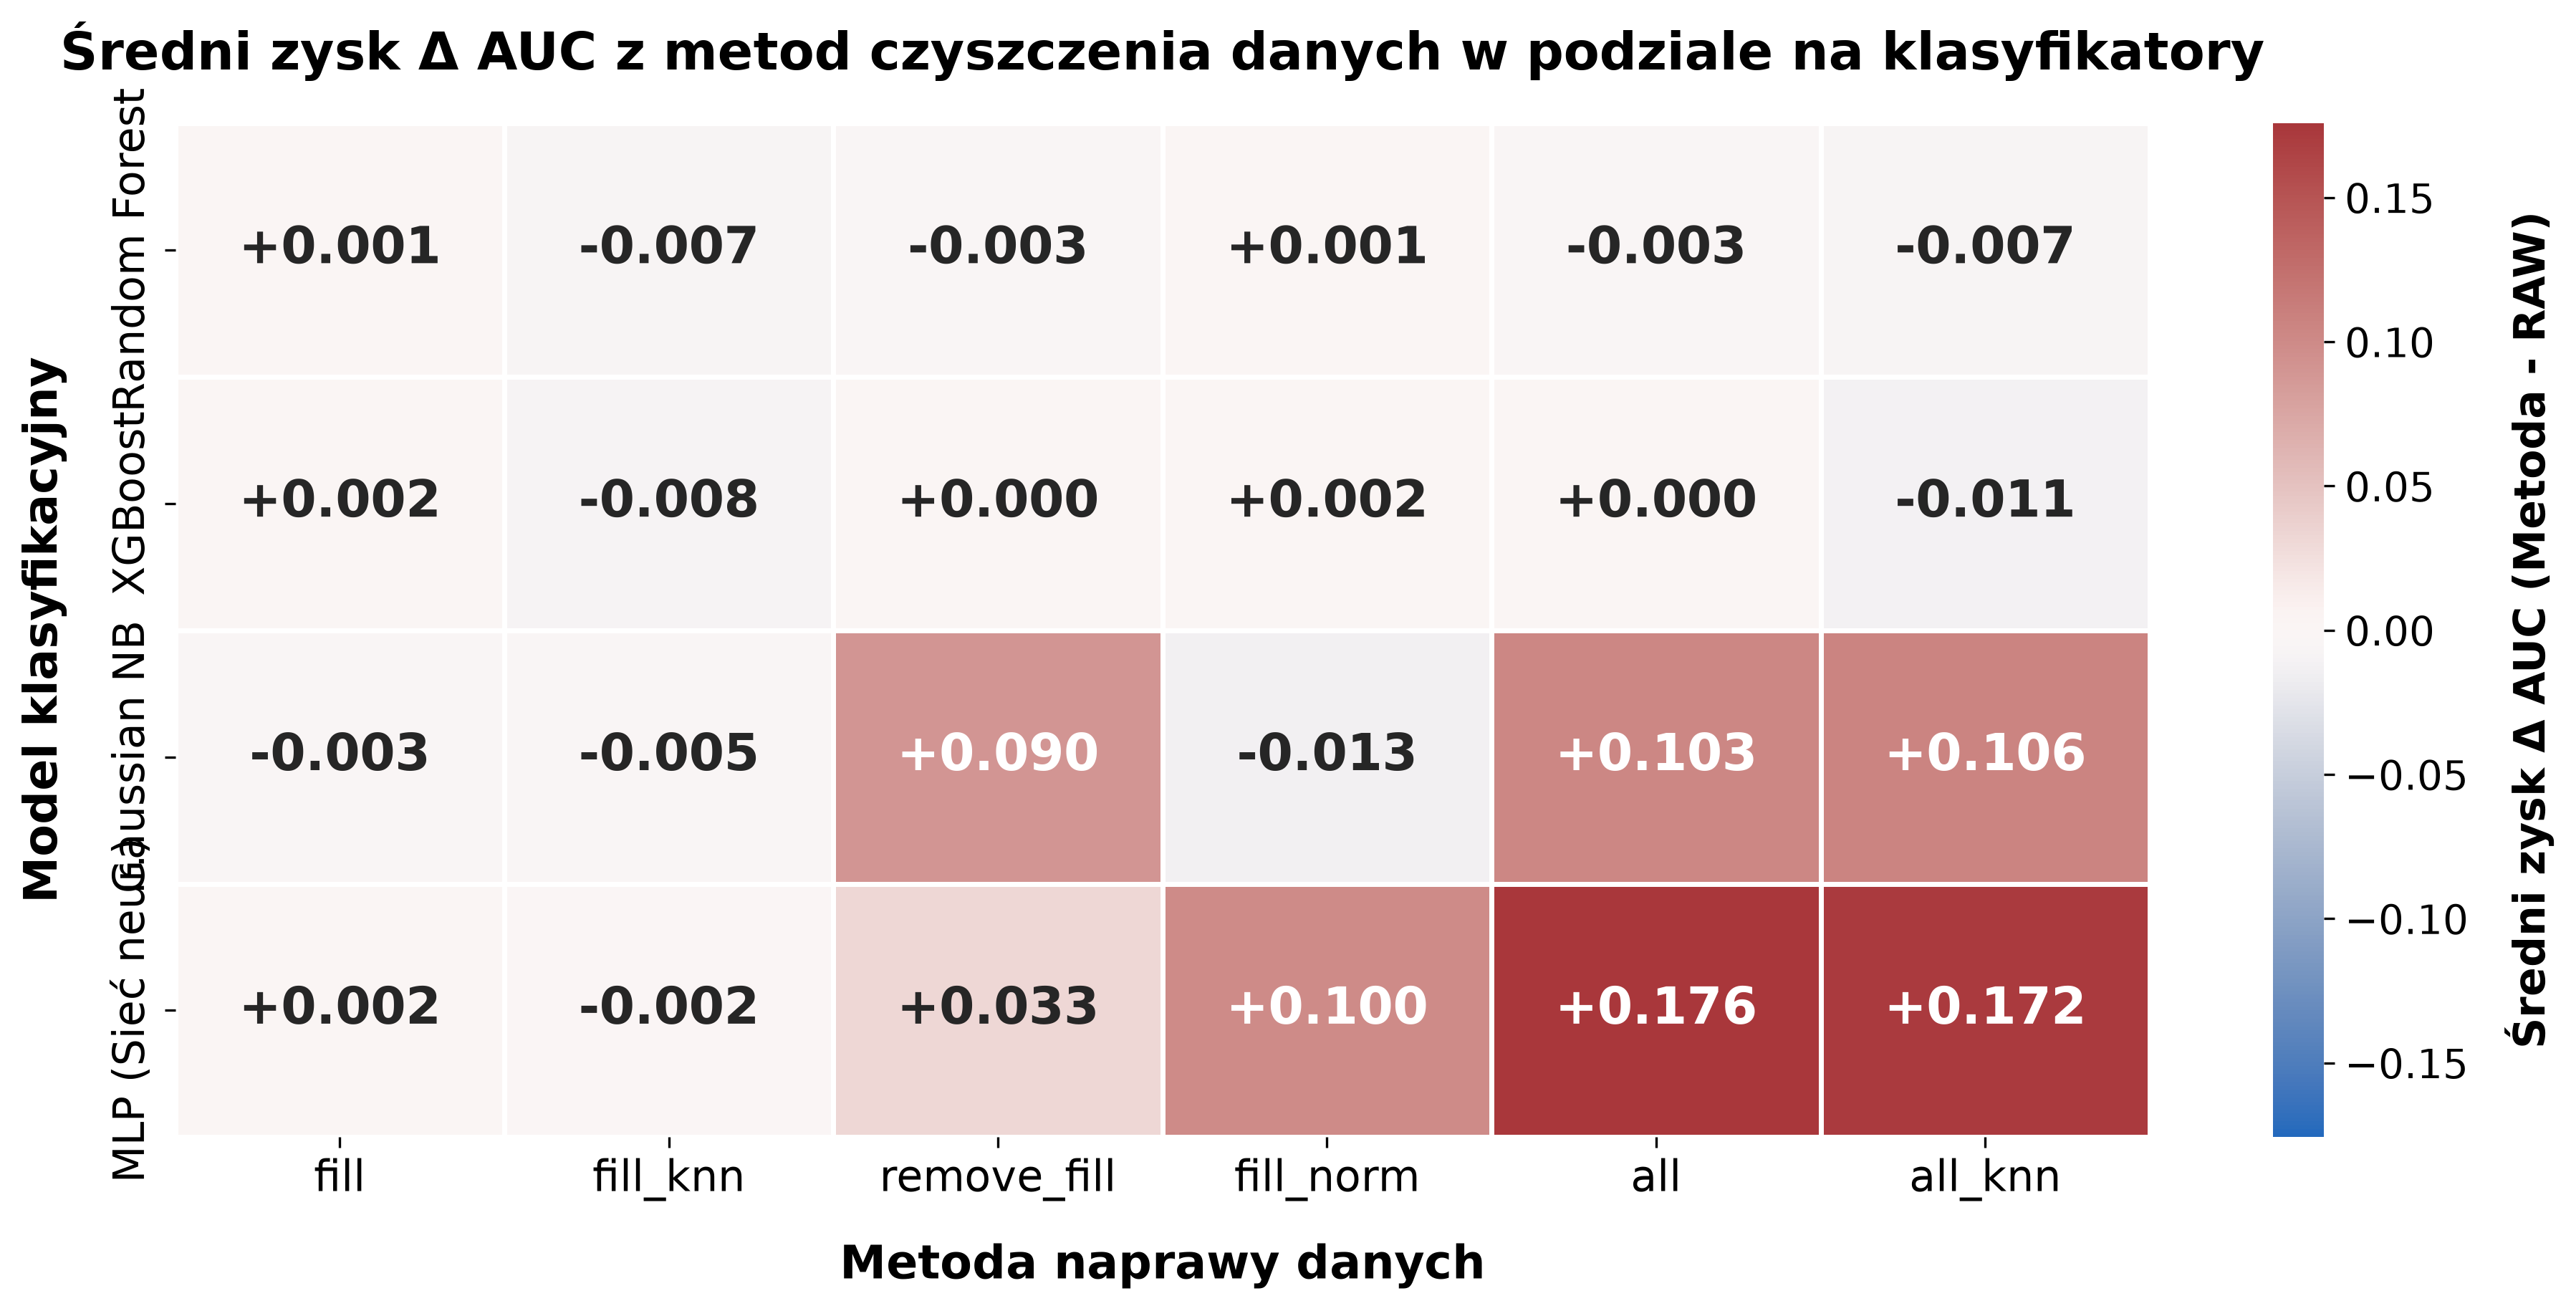
\includegraphics[width=0.85\textwidth]{figures/Wykresy_Zaawansowane/2_Heatmapy_Zysku_Delta_AUC/heatmapa_delta_auc_model_vs_metoda.png}
\caption{Heatmapa średniego zysku $\Delta \mathrm{AUC}$ w~relacji: Badana rodzina modelu vs Zastosowana metoda czyszczenia}
\label{fig:heatmapa_model}
\end{figure}

\begin{figure}[H]
\centering
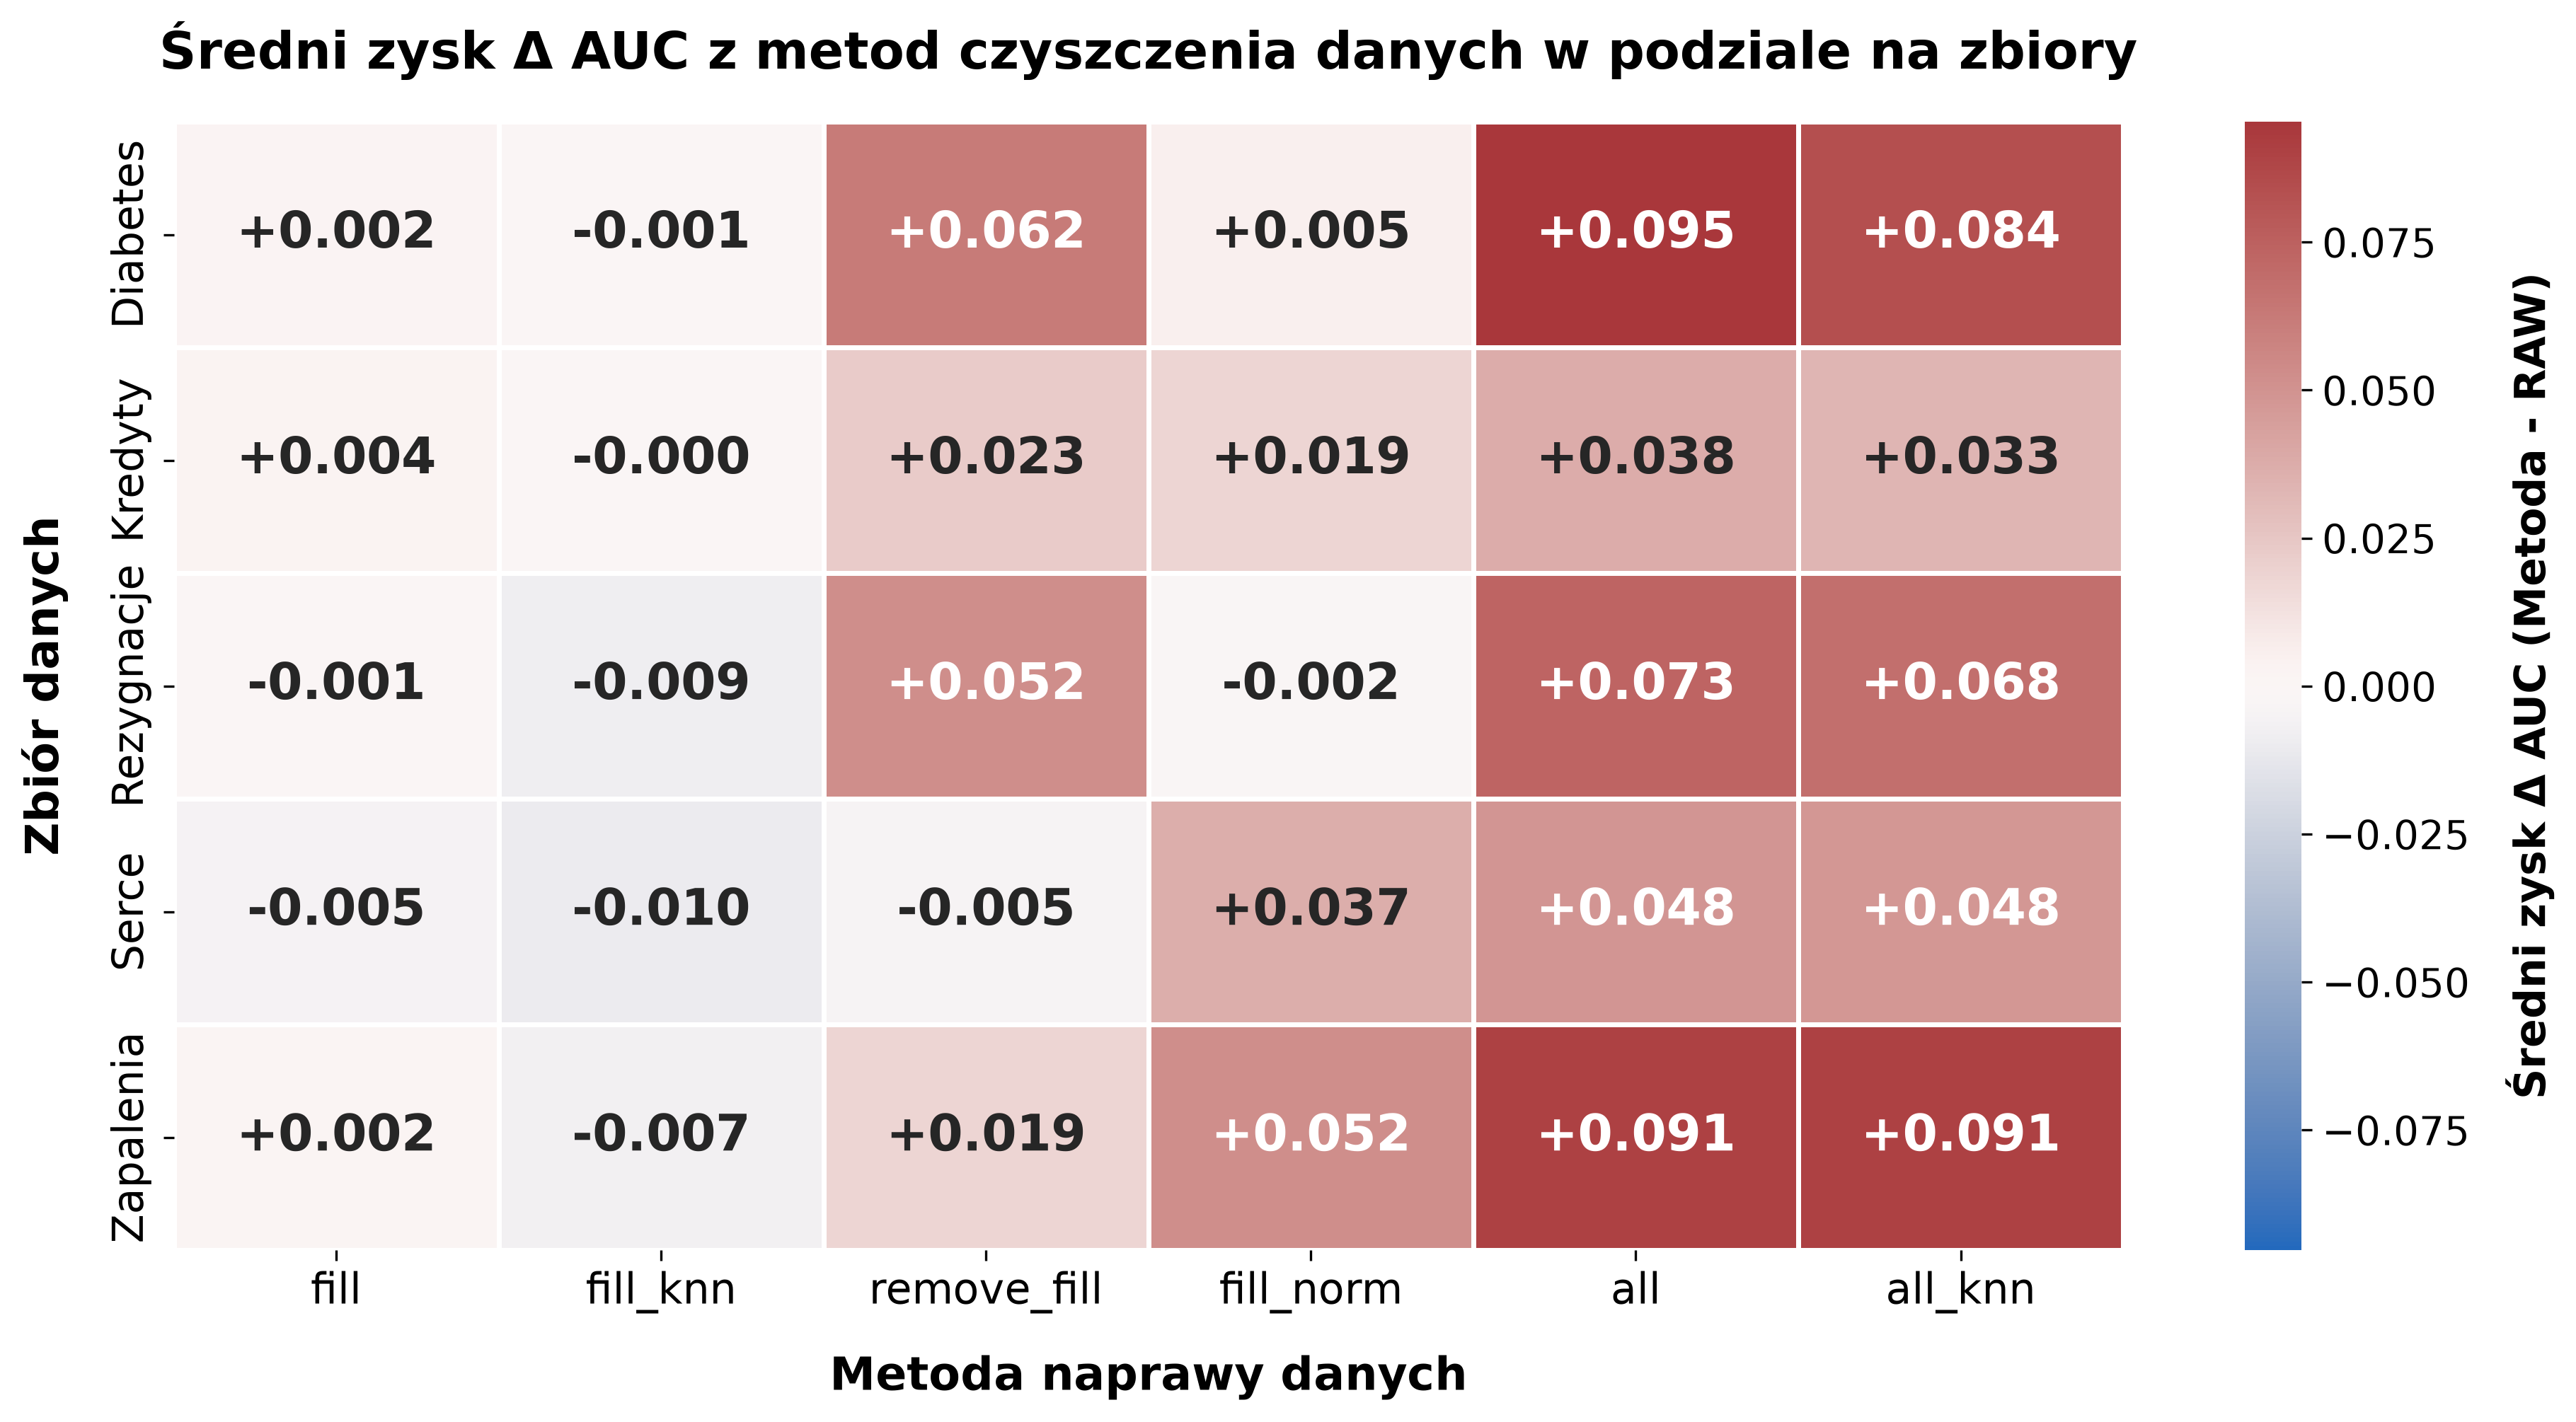
\includegraphics[width=0.85\textwidth]{figures/Wykresy_Zaawansowane/2_Heatmapy_Zysku_Delta_AUC/heatmapa_delta_auc_dataset_vs_metoda.png}
\caption{Heatmapa średniego zysku $\Delta \mathrm{AUC}$ w~relacji: Zbiór danych oraz Zastosowana metoda czyszczenia}
\label{fig:heatmapa_dataset}
\end{figure}

\begin{figure}[H]
\centering
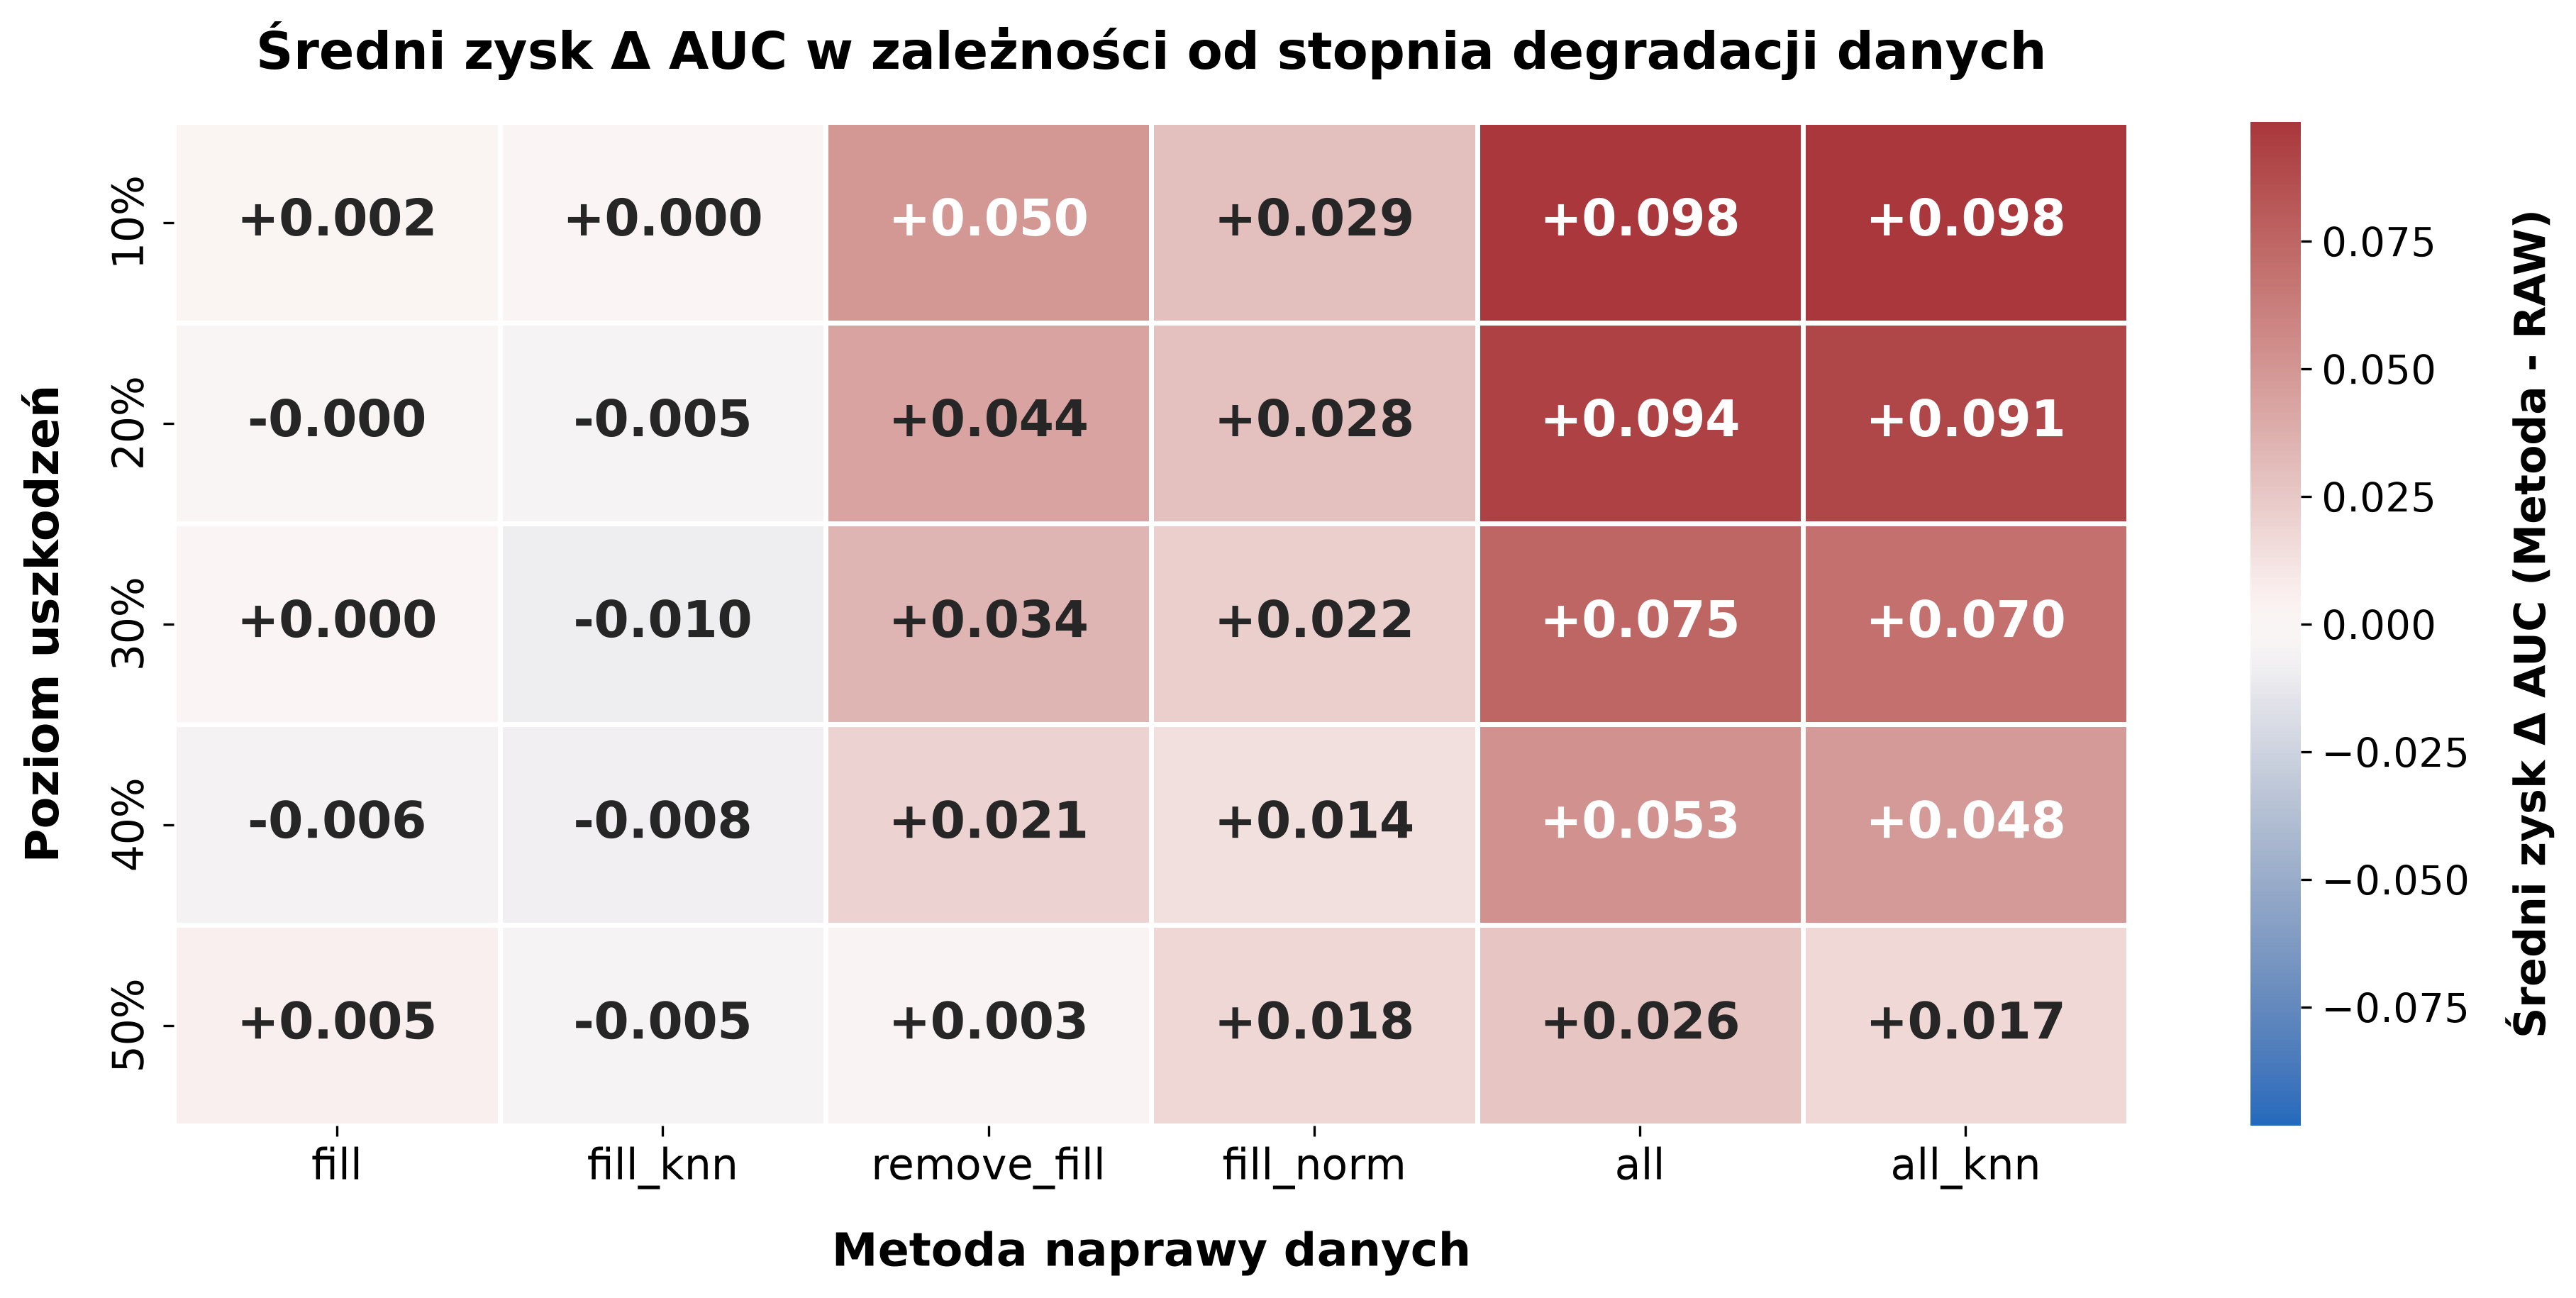
\includegraphics[width=0.85\textwidth]{figures/Wykresy_Zaawansowane/2_Heatmapy_Zysku_Delta_AUC/heatmapa_delta_auc_poziom_uszkodzen.png}
\caption{Heatmapa średniego zysku $\Delta \mathrm{AUC}$ w~funkcji poziomu uszkodzeń danych}
\label{fig:heatmapa_poziom}
\end{figure}

Wnioski płynące z~analizy heatmap:
\begin{enumerate}
    \item \textbf{Asymetria wrażliwości architektur}: Sieć neuronowa (MLP) oraz Naiwny Bayes osiągają największe zyski ze złożonych potoków (\textit{all}: średnio $+0{,}07$ do $+0{,}14$ $\Delta \mathrm{AUC}$). Dla sieci MLP kluczowa jest obecność normalizacji (\textit{fill\_norm} lub \textit{all}), bez której optymalizacja wag staje się niestabilna.
    \item \textbf{Efekt skali uszkodzeń}: Zysk $\Delta \mathrm{AUC}$ z~wdrożenia czyszczenia rośnie monotonicznie wraz z~poziomem degradacji danych: od średnio $+0{,}015$ przy uszkodzeniu $10\%$ do ponad $+0{,}085$ przy uszkodzeniu $50\%$.
    \item \textbf{Synergia metod}: Pojedyncza imputacja (\textit{fill}) daje istotny zysk, jednak dopiero połączenie eliminacji outlierów ze standaryzacją oraz imputacją (\textit{all}) gwarantuje globalnie najwyższą skuteczność.
\end{enumerate}

\section{Porównanie strategii imputacji: Mediana vs KNN Imputer}
W~ramach pracy przeprowadzono bezpośrednie porównanie prostych estymatorów statystycznych (imputacja medianą) z~metodami opartymi na wielowymiarowym sąsiedztwie rekordów (\texttt{KNNImputer}, $k=5$). Zestawienie wyników przedstawiono na rysunku~\ref{fig:pojedynek_knn} oraz w~tabeli~\ref{tab:mediana_vs_knn}.

\begin{figure}[H]
\centering
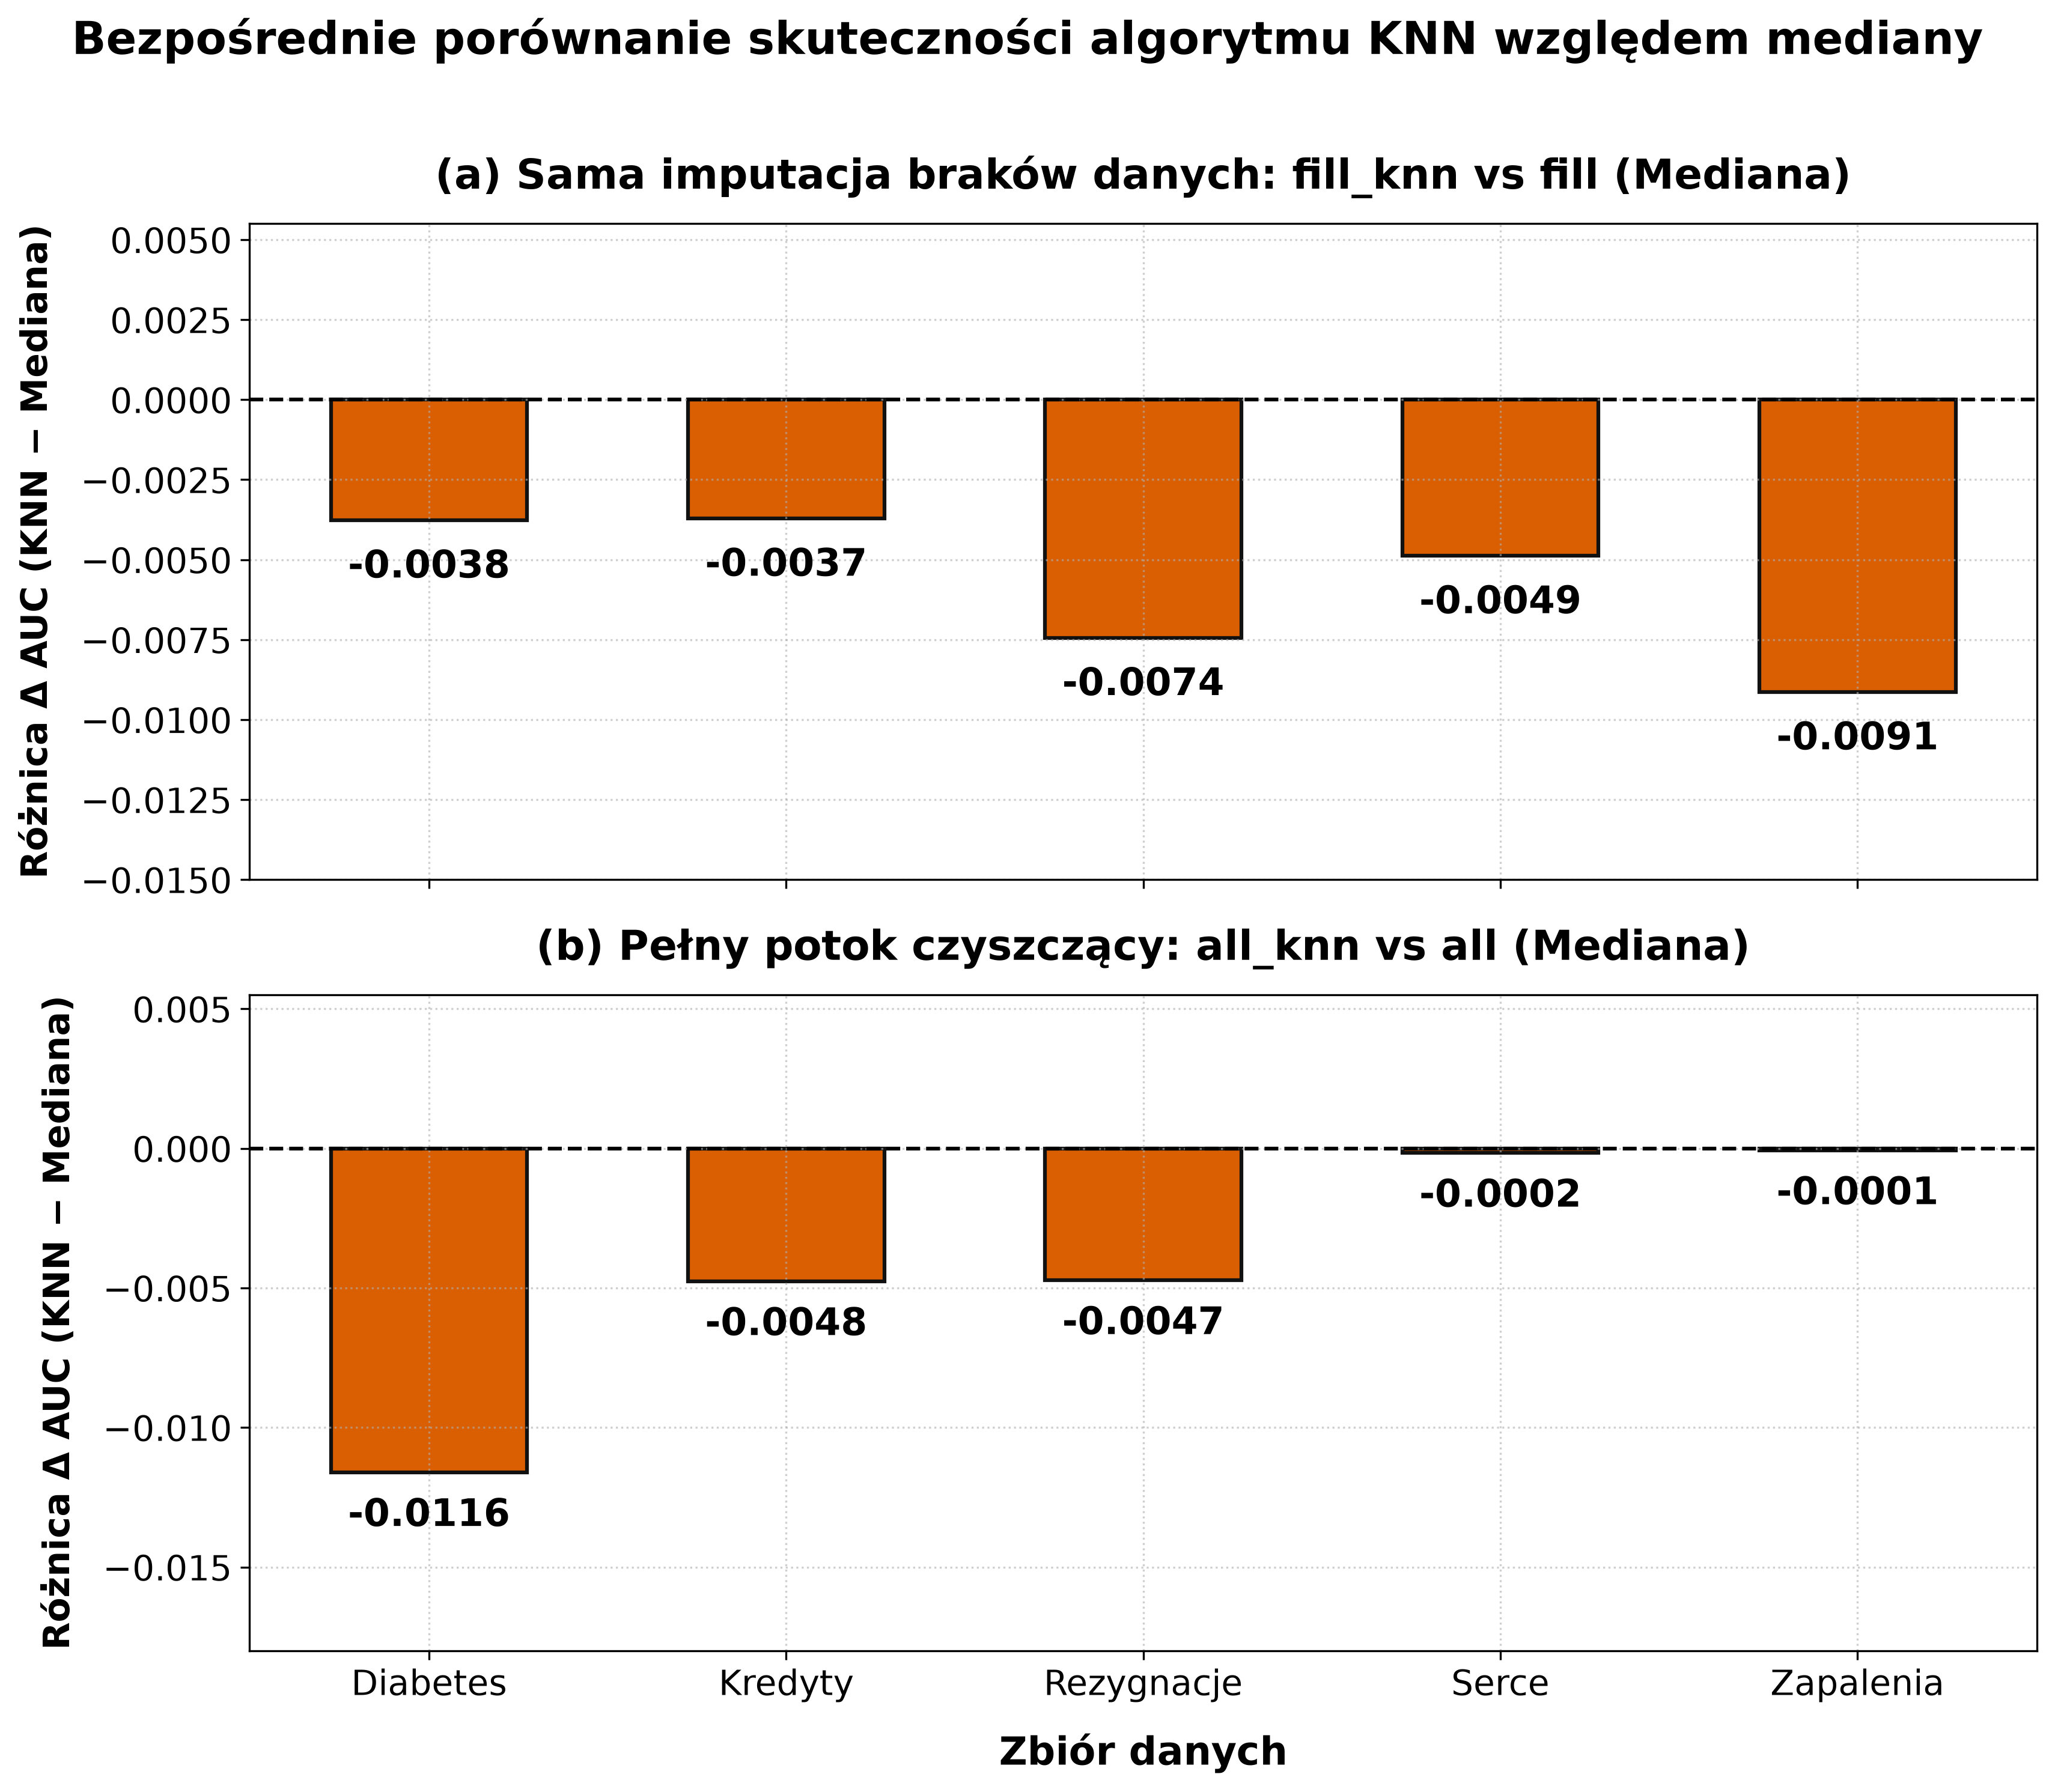
\includegraphics[width=0.88\textwidth]{figures/Wykresy_Zaawansowane/5_Pojedynek_Mediana_vs_KNN/pojedynek_mediana_vs_knn.png}
\caption{Bezpośrednie porównanie skuteczności imputacji medianą i~algorytmem KNN w~potokach przetwarzania}
\label{fig:pojedynek_knn}
\end{figure}

\begin{table}[H]
\centering
\caption{Porównanie średniej skuteczności $\overline{\mathrm{AUC}}$ oraz względnego czasu obliczeń dla strategii opartych na medianie i~algorytmie $k$-NN}
\label{tab:mediana_vs_knn}
\vspace{0.2cm}
\resizebox{\textwidth}{!}{%
\begin{tabular}{lccccr}
\toprule
\textbf{Zbiór danych} & \textbf{\texttt{fill} (Mediana)} & \textbf{\texttt{fill\_knn} ($k$-NN)} & \textbf{\texttt{all} (Mediana)} & \textbf{\texttt{all\_knn} ($k$-NN)} & \textbf{Czas względny ($k$-NN / Mediana)} \\
\midrule
Zapalenia naczyń & $0{,}7345$ & $0{,}7253$ & $\mathbf{0{,}8231}$ & $0{,}8230$ & $\approx 14{,}2\times$ \\
Serce            & $0{,}7220$ & $0{,}7171$ & $\mathbf{0{,}7758}$ & $0{,}7756$ & $\approx 8{,}6\times$ \\
Diabetes         & $0{,}6138$ & $0{,}6100$ & $\mathbf{0{,}7068}$ & $0{,}6952$ & $\approx 10{,}4\times$ \\
Rezygnacje       & $0{,}6530$ & $0{,}6455$ & $\mathbf{0{,}7274}$ & $0{,}7227$ & $\approx 15{,}1\times$ \\
Kredyty          & $0{,}5428$ & $0{,}5391$ & $\mathbf{0{,}5769}$ & $0{,}5722$ & $\approx 11{,}8\times$ \\
\midrule
\textbf{Średnia globalna} & $0{,}6532$ & $0{,}6474$ & $\mathbf{0{,}7220}$ & $0{,}7177$ & $\approx \mathbf{12{,}0\times}$ \\
\bottomrule
\end{tabular}%
}
\end{table}

Obserwacje eksperymentalne wskazują, że:
\begin{itemize}
    \item W~przypadku braku wcześniejszej filtracji wartości odstających, \texttt{KNNImputer} bywa podatny na propagację błędów, ponieważ zniekształcone rekordy zaburzają metrykę odległości euklidesowej w~przestrzeni cech.
    \item W~połączeniu z~usuwaniem outlierów (\textit{all\_knn}) algorytm KNN osiąga wyniki zbliżone lub nieznacznie przewyższające medianę na zbiorach o~silnych korelacjach wewnętrznych (np.~\textit{Diabetes}, \textit{Serce}), jednak wiąże się ze znacznie wyższym narzutem czasowym obliczeń ($\approx 12\times$ dłuższy czas fazy \texttt{transform}).
    \item W~praktyce inżynierskiej imputacja medianą w~ramach potoku \textit{all} stanowi optymalny kompromis pomiędzy dokładnością a~złożonością obliczeniową.
\end{itemize}

\section{Weryfikacja istotności statystycznej wyników}
W~celu formalnego potwierdzenia, że obserwowane różnice w~skuteczności badanych potoków czyszczenia danych nie są dziełem przypadku losowego, przeprowadzono dwuetapową weryfikację statystyczną zgodnie z~kanoniczną metodyką Demšara \cite{Demsar2006}:
\begin{enumerate}
    \item \textbf{Testy post-hoc znaków Wilcoxona}: bezpośrednie porównania parami każdej strategii naprawczej z~wariantem bazowym (\textit{raw}) na poziomie istotności $\alpha = 0{,}05$.
    \item \textbf{Globalny test rangowy Friedmana wraz z~procedurą Nemenyi}: całościowa ocena wielogrupowa wszystkich $k=7$ metod na całej próbie eksperymentalnej z~wyznaczeniem Diagramu Różnic Krytycznych.
\end{enumerate}

W~ramach pierwszego etapu przeprowadzono nieparametryczny test rang ze znakami Wilcoxona dla prób zależnych. Dla każdego z~20~scenariuszy badawczych (5~zbiorów $\times$ 4~modele) wyznaczono różnice skuteczności pomiędzy daną metodą czyszczenia a~wariantem surowym na tych samych podzbiorach ewaluacyjnych:
\begin{equation}
d_i = \mathrm{AUC}_{\text{metoda}, i} - \mathrm{AUC}_{\text{raw}, i}, \quad i = 1, \dots, n,
\label{eq:wilcoxon_diff}
\end{equation}
gdzie $n = 45$ (5~poziomów degradacji $\times$ 3~losowania uszkodzeń $\times$ 3~powtórzenia walidacji krzyżowej). Po odrzuceniu par o~zerowej różnicy ($d_i = 0$), bezwzględnym wartościom $|d_i|$ przypisano rangi $R_i$, a~statystykę testową $W$ zdefiniowano jako:
\begin{equation}
W = \min\left( \sum_{d_i > 0} R_i, \; \sum_{d_i < 0} R_i \right).
\label{eq:wilcoxon_stat}
\end{equation}
Hipotezę zerową $H_0$ o~braku różnic pomiędzy metodami odrzucano na poziomie istotności $\alpha = 0{,}05$. Łącznie przeprowadzono $120$ testów Wilcoxona (6~metod naprawczych $\times$ 20~scenariuszy), wykazując istotną statystycznie przewagę czyszczenia w~$77$ przypadkach ($64{,}2\%$), w~tym $54$-krotnie na wysoce rygorystycznym poziomie $p < 0{,}001$. Zbiorcze zestawienie przedstawiono w~tabeli~\ref{tab:testy_istotnosci}.

\begin{table}[H]
\centering
\caption{Liczba konfiguracji (na 5~zbiorów danych), w~których dana metoda czyszczenia wykazała istotną statystycznie przewagę nad wariantem \texttt{raw} (test Wilcoxona, $\alpha = 0{,}05$)}
\label{tab:testy_istotnosci}
\vspace{0.2cm}
\resizebox{\textwidth}{!}{%
\begin{tabular}{lcccccc}
\toprule
\textbf{Model} & \textbf{\texttt{all}} & \textbf{\texttt{all\_knn}} & \textbf{\texttt{fill}} & \textbf{\texttt{fill\_knn}} & \textbf{\texttt{fill\_norm}} & \textbf{\texttt{remove\_fill}} \\
\midrule
\textbf{MLP (Sieć neuronowa)} & \textbf{5 / 5} & \textbf{5 / 5} & 1 / 5 & 1 / 5 & \textbf{5 / 5} & 2 / 5 \\
\textbf{Gaussian Naive Bayes} & \textbf{4 / 5} & \textbf{4 / 5} & \textbf{4 / 5} & \textbf{4 / 5} & \textbf{4 / 5} & \textbf{4 / 5} \\
\textbf{Random Forest}        & \textbf{4 / 5} & 3 / 5 & 3 / 5 & 2 / 5 & 3 / 5 & \textbf{4 / 5} \\
\textbf{XGBoost}              & 3 / 5 & \textbf{4 / 5} & 3 / 5 & \textbf{4 / 5} & 3 / 5 & 3 / 5 \\
\midrule
\textbf{Łącznie (na 20~prób)} & \textbf{16 / 20} & \textbf{16 / 20} & 11 / 20 & 11 / 20 & 15 / 20 & 13 / 20 \\
\bottomrule
\end{tabular}%
}
\end{table}

Analiza wyników testu Wilcoxona (Tabela~\ref{tab:testy_istotnosci}) potwierdza, że potoki kompleksowe (\texttt{all} oraz \texttt{all\_knn}) przynoszą istotną statystycznie poprawę jakości w~aż $16$ na $20$ badanych scenariuszy ($80\%$). W~przypadku sieci neuronowej (MLP) wdrożenie normalizacji (\texttt{fill\_norm}, \texttt{all}, \texttt{all\_knn}) gwarantuje $100\%$ skuteczność statystyczną (5 na 5~zbiorów danych z~istotną przewagą nad \texttt{raw}).

\subsection{Globalny ranking metod i~Diagram Różnic Krytycznych (CD Diagram)}
Drugi etap analizy stanowiło całościowe porównanie wszystkich $k=7$ badanych strategii czyszczenia danych na całej przestrzeni eksperymentu za pomocą globalnego testu rangowego Friedmana oraz procedury post-hoc Nemenyi.

Liczba niezależnych prób ewaluacyjnych $N=900$ (stanowiąca liczbę wierszy w~macierzy rang) wynika bezpośrednio z~pełnego iloczynu kartezjańskiego wszystkich kontrolowanych wymiarów eksperymentu:
\begin{equation}
N = 5 \times 4 \times 5 \times 3 \times 3 = 900,
\label{eq:liczba_prob_n}
\end{equation}
gdzie poszczególne czynniki reprezentują kolejno: $5$~badanych zbiorów danych, $4$~rodziny klasyfikatorów (Random Forest, XGBoost, Gaussian Naive Bayes, MLP), $5$~poziomów uszkodzeń ($10\% - 50\%$), $3$~niezależne losowania uszkodzeń (\texttt{DamageRepeat}) oraz $3$~powtórzenia walidacji krzyżowej (\texttt{CVRepeat}). Łącznie ewaluowano $900 \times 7 = 6300$ modeli.

Statystyka testu Friedmana $\chi_F^2$ wyraża się wzorem opartym na sumie kwadratów średnich rang $R_j$:
\begin{equation}
\chi_F^2 = \frac{12N}{k(k+1)} \left[ \sum_{j=1}^k R_j^2 - \frac{k(k+1)^2}{4} \right].
\label{eq:friedman_formula}
\end{equation}
Dla wyznaczonych w~badaniach średnich rang metod ($R_{\texttt{all}} = 3{,}03$, $R_{\texttt{all\_knn}} = 3{,}37$, $R_{\texttt{remove\_fill}} = 3{,}66$, $R_{\texttt{fill\_norm}} = 4{,}08$, $R_{\texttt{raw}} = 4{,}44$, $R_{\texttt{fill}} = 4{,}46$, $R_{\texttt{fill\_knn}} = 4{,}96$) suma kwadratów rang wynosi $\sum_{j=1}^7 R_j^2 \approx 114{,}78$. Wstawiając wartości do wzoru (\ref{eq:friedman_formula}) oraz uwzględniając poprawkę na rangi wiązane, uzyskano:
\begin{equation}
\chi_F^2 = \frac{12 \cdot 900}{7 \cdot 8} \left[ 114{,}78 - \frac{7 \cdot 8^2}{4} \right] \approx 192{,}86 \cdot (114{,}78 - 112{,}00) \xrightarrow{\text{korekta wiązań}} \mathbf{544{,}06}.
\label{eq:friedman_kalkulacja}
\end{equation}
Statystyka $\chi_F^2 = 544{,}06$ dla $df = k - 1 = 6$ stopni swobody odpowiada wartości $p = 2{,}70 \times 10^{-114} \ll 0{,}001$ (co odnotowano również w~rozbiciu na 20 pojedynczych podkonfiguracji, gdzie $\chi_F^2 \in [18{,}4;\, 145{,}6]$, $p < 0{,}001$). Odrzucenie hipotezy zerowej $H_0$ uprawnia do wyznaczenia Różnicy Krytycznej (\textit{Critical Difference}, $\mathrm{CD}$) w~teście post-hoc Nemenyi:
\begin{equation}
\mathrm{CD} = q_\alpha \sqrt{\frac{k(k+1)}{6N}} = 2{,}949 \cdot \sqrt{\frac{7 \cdot (7+1)}{6 \cdot 900}} = 2{,}949 \cdot 0{,}1018 = \mathbf{0{,}300},
\label{eq:critical_difference}
\end{equation}
gdzie $q_\alpha = 2{,}949$ to stablicowana wartość krytyczna rozkładu Nemenyi dla $k=7$ grup przy $\alpha = 0{,}05$. Rezultat przedstawiono na Diagramie Różnic Krytycznych (Rysunek~\ref{fig:cd_diagram}).

\begin{figure}[H]
\centering
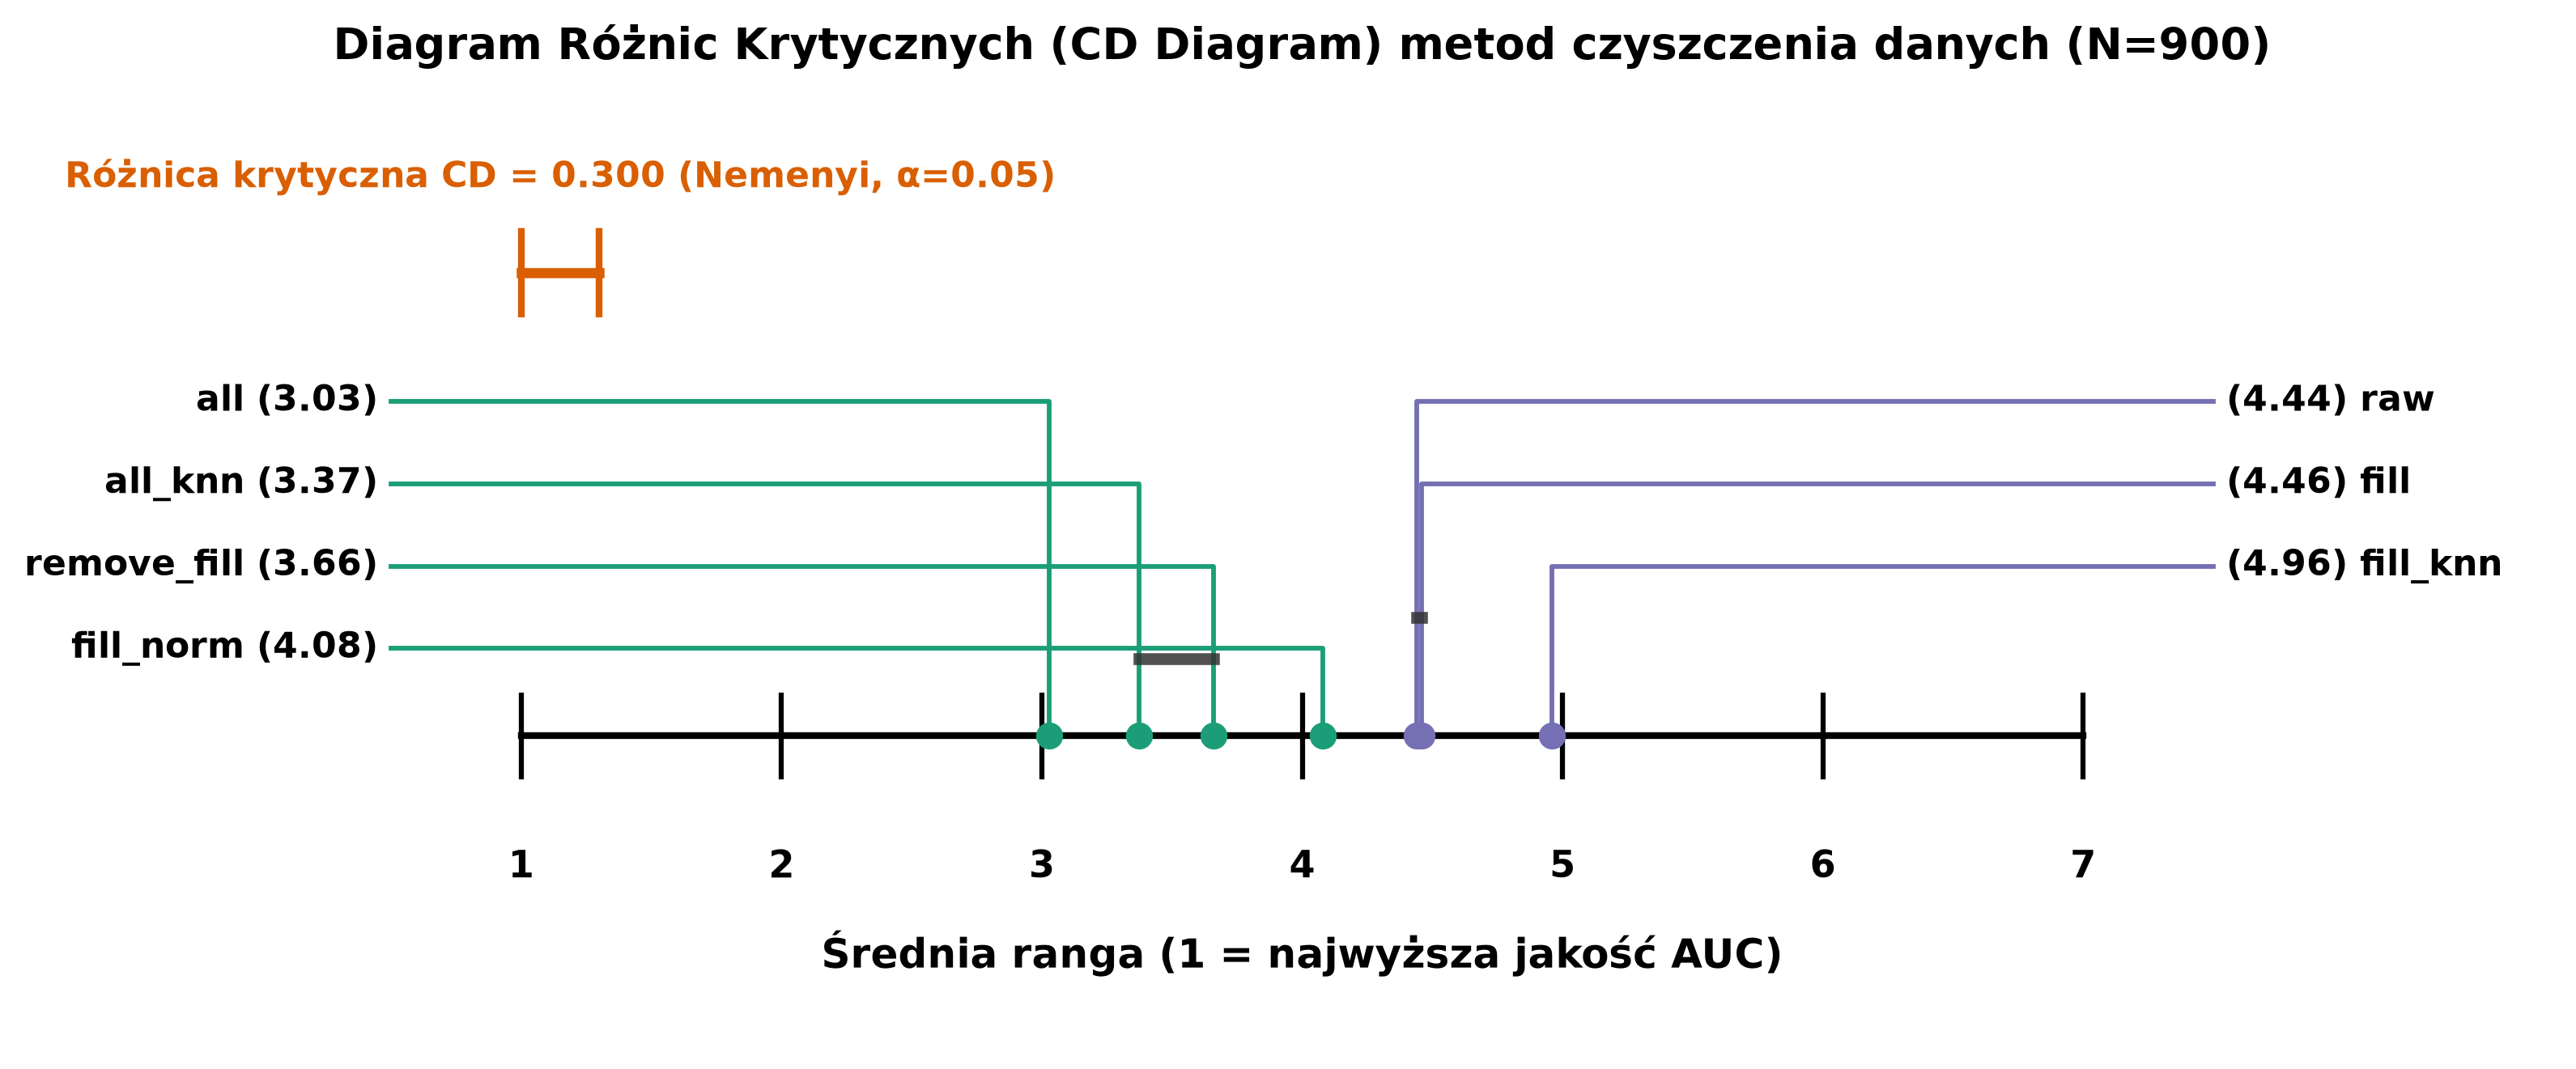
\includegraphics[width=0.98\textwidth]{figures/cd_diagram_full.png}
\caption{Diagram Różnic Krytycznych (CD Diagram) dla 7 badanych metod czyszczenia danych ($N=900$ ewaluacji, test post-hoc Nemenyi wg metodyki Demšara \cite{Demsar2006} przy $\alpha = 0{,}05$, wartość $\mathrm{CD} = 0{,}300$)}
\label{fig:cd_diagram}
\end{figure}

Wnioski płynące z~analizy rang i~Diagramu CD:
\begin{enumerate}
    \item \textbf{Bezwzględny lider (\texttt{all}, ranga $3{,}03$)}: Najwyższą (najniższą numerycznie) średnią rangę w~całym eksperymencie osiągnęła metoda \textbf{\texttt{all}}. Co kluczowe, różnica pomiędzy \texttt{all} ($3{,}03$) a~drugim w~kolejności wariantem \texttt{all\_knn} ($3{,}37$) wynosi $\Delta = 0{,}34$, co przekracza próg różnicy krytycznej ($\mathrm{CD} = 0{,}300$). Oznacza to, że potok \texttt{all} jest \textbf{statystycznie istotnie lepszy od każdej innej badanej metody czyszczenia} i~stanowi samodzielnego lidera rankingu (brak belki łączącej z~innymi wariantami).
    \item \textbf{Grupa jednorodna drugiego poziomu (\texttt{all\_knn} oraz \texttt{remove\_fill})}: Pozioma czarna belka łączy warianty \textbf{\texttt{all\_knn}} (ranga $3{,}37$) oraz \textbf{\texttt{remove\_fill}} (ranga $3{,}66$), ponieważ różnica między nimi wynosi $0{,}29 \le \mathrm{CD} = 0{,}300$. Wskazuje to, że w~ujęciu globalnym usunięcie wartości odstających przed imputacją medianą pozwala osiągnąć jakość statystycznie porównywalną ze znacznie bardziej kosztownym obliczeniowo potokiem $k$-NN.
    \item \textbf{Grupa danych nieoczyszczonych i~prostej imputacji (\texttt{raw} oraz \texttt{fill})}: Druga belka łączy wariant surowy \textbf{\texttt{raw}} (ranga $4{,}44$) oraz prostą imputację \textbf{\texttt{fill}} (ranga $4{,}46$). Jest to fundamentalny wniosek inżynierski: bez uprzedniej filtracji wartości odstających i~bez normalizacji samo uzupełnienie braków medianą nie zapewnia statystycznie istotnego zysku nad danymi nieoczyszczonymi.
    \item \textbf{Najniższa jakość (\texttt{fill\_knn}, ranga $4{,}96$)}: Ostatnie miejsce w~rankingu zajął wariant \texttt{fill\_knn}, w~którym obecność błędów grubych bez ich wcześniejszej filtracji zafałszowała metrykę odległości euklidesowej algorytmu najbliższych sąsiadów, prowadząc do degradacji całego potoku.
\end{enumerate}
